% =============================================================================
% BMED365 (Spring 2027) — Master's-Level Companion Technical Report ("Thesis + Code")
% Canonical Geometric Preprocessing for 3D Biomedical Instance Segmentation
% on 7T MRI: Isotropic Reslicing, Rigid Polar Alignment (f = f_2 o f_1),
% Invertible Label Resampling (f^-1), Neurosymbolic Ablation, and
% AI-Assisted Scientific Coding
%
% Compile cleanly with TeX Live 2025:
%   pdflatex canonical-kiwi-report.tex
%   bibtex canonical-kiwi-report
%   pdflatex canonical-kiwi-report.tex
%   pdflatex canonical-kiwi-report.tex
% =============================================================================
\documentclass[10pt,a4paper]{article}

\usepackage[utf8]{inputenc}
\usepackage[T1]{fontenc}
\usepackage[english]{babel}
\usepackage{lmodern}
\usepackage{microtype}
\usepackage{graphicx}
\usepackage{booktabs}
\usepackage{xltabular}
\usepackage{tabularx}
\usepackage{array}
\usepackage{multirow}
\usepackage[table]{xcolor}
\usepackage{amsmath,amssymb,mathtools}
\usepackage{enumitem}
\usepackage[margin=2.05cm,top=2.15cm,bottom=2.15cm,headheight=14.5pt]{geometry}
\usepackage{fancyhdr}
\usepackage{lastpage}
\usepackage{titlesec}
\usepackage[most]{tcolorbox}
\usetikzlibrary{arrows.meta,positioning,shapes.geometric,fit,backgrounds}
\usepackage{listings}
\usepackage{float}
\usepackage[font=small,labelfont={bf,color=uibblue},skip=5pt]{caption}
\usepackage{csquotes}
\usepackage[hyphens]{url}

% Clickable bibliography via biblatex + bibtex (portable across macOS/Linux/Overleaf;
% full clickable DOIs, arXiv eprints, numeric-comp citations, and page backrefs)
\usepackage[
    backend=bibtex,
    style=numeric-comp,
    sorting=none,
    maxbibnames=6,
    minbibnames=3,
    giveninits=true,
    doi=true,
    isbn=false,
    url=true,
    eprint=true,
    backref=true
]{biblatex}
\addbibresource{canonical-references.bib}

% Hyperref MUST come after biblatex for clickable citations, DOIs, eprints, TOC & backrefs
\usepackage[
    colorlinks=true,
    linkcolor=uibblue,
    citecolor=uibblue,
    urlcolor=uibred,
    bookmarksnumbered=true,
    bookmarksopen=true,
    pdfauthor={Arvid Lundervold (University of Bergen & MMIV) -- BMED365 Spring 2027},
    pdftitle={Canonical Geometric Preprocessing for 3D Biomedical Instance Segmentation on 7T MRI},
    pdfsubject={BMED365 Companion Technical Report: Isotropic Reslicing, Rigid Polar Alignment, Invertible Resampling, Neurosymbolic Ablation, and AI-Assisted Scientific Coding}
]{hyperref}
\def\UrlBreaks{\do\/\do-\do_\do.}
% Allow clean line breaks after underscores in long filenames & Python identifiers
\let\origunderscore\_
\renewcommand{\_}{\origunderscore\allowbreak}

% =============================================================================
% COLOR PALETTE (University of Bergen / MMIV / BMED365 House Style)
% =============================================================================
\definecolor{uibblue}{RGB}{0, 61, 115}
\definecolor{uibred}{RGB}{175, 28, 44}
\definecolor{kiwigreen}{RGB}{27, 138, 90}
\definecolor{amberwarn}{RGB}{165, 95, 0}
\definecolor{amberbg}{RGB}{255, 250, 240}
\definecolor{lightgray}{RGB}{246, 248, 250}
\definecolor{rowalt}{RGB}{243, 247, 252}
\definecolor{codebg}{RGB}{245, 248, 252}
\definecolor{codehdr}{RGB}{224, 234, 246}
\definecolor{codekw}{RGB}{0, 75, 145}
\definecolor{codestr}{RGB}{155, 35, 45}
\definecolor{codecmt}{RGB}{90, 105, 118}
\definecolor{tealaccent}{RGB}{12, 112, 128}

% =============================================================================
% TYPOGRAPHY, HEADERS, FOOTERS & CALLOUT BOXES
% =============================================================================
\setlength{\parindent}{0pt}
\setlength{\parskip}{0.46em}
\setlength{\emergencystretch}{1.8em}
\setlist[itemize]{topsep=3pt,itemsep=2.2pt,leftmargin=1.5em}
\setlist[enumerate]{topsep=3pt,itemsep=2.2pt,leftmargin=1.7em}

\newcolumntype{L}[1]{>{\raggedright\arraybackslash}p{#1}}
\newcolumntype{C}[1]{>{\centering\arraybackslash}p{#1}}
\newcolumntype{R}[1]{>{\raggedleft\arraybackslash}p{#1}}
\newcolumntype{Y}{>{\raggedright\arraybackslash}X}

\titleformat{\section}{\Large\bfseries\color{uibblue}}{\thesection}{0.7em}{}[\vspace{2pt}\color{uibblue!45}\titlerule]
\titleformat{\subsection}{\large\bfseries\color{uibblue!88!black}}{\thesubsection}{0.55em}{}
\titleformat{\subsubsection}{\normalsize\bfseries\color{uibblue!75!black}}{\thesubsubsection}{0.5em}{}
\titlespacing*{\section}{0pt}{1.3em}{0.5em}
\titlespacing*{\subsection}{0pt}{0.9em}{0.32em}
\titlespacing*{\subsubsection}{0pt}{0.6em}{0.22em}

\pagestyle{fancy}
\fancyhf{}
\fancyhead[L]{\footnotesize\textcolor{gray}{BMED365 (Spring 2027) $\cdot$ Canonical 7\,T MRI Report}}
\fancyhead[R]{\footnotesize\textcolor{gray}{\nouppercase{\leftmark}}}
\fancyfoot[L]{\footnotesize\textcolor{gray}{University of Bergen \& MMIV $\cdot$ \href{https://github.com/arvidl/BMED365-2027}{\textcolor{gray}{github.com/arvidl/BMED365-2027}}}}
\fancyfoot[R]{\footnotesize\textcolor{gray}{Page \thepage{} of \pageref{LastPage}}}
\renewcommand{\headrulewidth}{0.4pt}
\renewcommand{\footrulewidth}{0.25pt}
\renewcommand{\sectionmark}[1]{\markboth{\thesection.\ #1}{}}

\newtcolorbox{keybox}[1][]{
    enhanced, breakable,
    colback=lightgray, colframe=uibblue,
    colbacktitle=uibblue, coltitle=white,
    fonttitle=\bfseries\small, title={#1},
    boxrule=0.65pt, arc=2.5pt, left=8pt, right=8pt, top=5.5pt, bottom=5.5pt
}

\newtcolorbox{clinbox}[1][]{
    enhanced, breakable,
    colback=amberbg, colframe=amberwarn,
    colbacktitle=amberwarn, coltitle=white,
    fonttitle=\bfseries\small, title={#1},
    boxrule=0.65pt, arc=2.5pt, left=8pt, right=8pt, top=5.5pt, bottom=5.5pt
}

\newtcolorbox{insightbox}[1][]{
    enhanced, breakable,
    colback=kiwigreen!6, colframe=kiwigreen!80!black,
    colbacktitle=kiwigreen!80!black, coltitle=white,
    fonttitle=\bfseries\small, title={#1},
    boxrule=0.65pt, arc=2.5pt, left=8pt, right=8pt, top=5.5pt, bottom=5.5pt
}

\newtcolorbox{didacticbox}[1][]{
    enhanced, breakable,
    colback=tealaccent!5, colframe=tealaccent!85!black,
    colbacktitle=tealaccent!85!black, coltitle=white,
    fonttitle=\bfseries\small, title={#1},
    boxrule=0.6pt, arc=2.5pt, left=8pt, right=8pt, top=5.5pt, bottom=5.5pt
}

\lstdefinestyle{pybmed}{
    language=Python,
    basicstyle=\ttfamily\scriptsize,
    keywordstyle=\bfseries\color{codekw},
    stringstyle=\color{codestr},
    commentstyle=\itshape\color{codecmt},
    showstringspaces=false,
    breaklines=true,
    breakatwhitespace=false,
    breakindent=12pt,
    columns=fullflexible,
    keepspaces=true,
    upquote=true
}

\newcommand{\ghblob}{https://github.com/arvidl/BMED365-2027/blob/main}
\newcommand{\colabbase}{https://colab.research.google.com/github/arvidl/BMED365-2027/blob/main}
\newcommand{\repodir}{Lab4-Comp-Imag/Kiwi-challenge/docs/neurosymbolic-report}
\newcommand{\nbref}[1]{\href{\ghblob/\repodir/notebooks/#1}{\texttt{#1}}}
\newcommand{\colablink}[2]{\href{\colabbase/\repodir/notebooks/#1}{#2}}
\newcommand{\natrep}{\href{\ghblob/\repodir/neurosymbolic-kiwi-report.pdf}{\texttt{neurosymbolic-\allowbreak kiwi-\allowbreak report.pdf}}}

\begin{document}

% =============================================================================
% FORMAL TITLE / COVER PAGE
% =============================================================================
\thispagestyle{empty}
\vspace*{-0.55cm}

\begin{tcolorbox}[
    enhanced, colback=uibblue, colframe=uibblue,
    arc=4pt, left=13pt, right=13pt, top=9pt, bottom=9pt
]
{\small\sffamily\bfseries\color{white!82} UNIVERSITY OF BERGEN (UiB) $\;\cdot\;$ MOHN MEDICAL IMAGING AND VISUALIZATION CENTRE (MMIV)}\\[2pt]
{\footnotesize\sffamily\color{white!76} BMED365 --- Computational Imaging, Modeling and AI in Biomedicine (Spring 2027) $\;\cdot\;$ Companion Technical Report (Canonical Representation)}\\[10pt]
{\LARGE\bfseries\color{white} Canonical Geometric Preprocessing for 3D Biomedical Instance Segmentation on 7\,T MRI}\\[4pt]
{\large\color{white!92} Isotropic Reslicing, Rigid Polar Alignment ($f = f_2 \circ f_1$), Invertible Label Resampling ($f^{-1}$), Multi-Seed Neurosymbolic Ablation, and AI-Assisted Scientific Coding}
\end{tcolorbox}

\vspace{0.22cm}

{\footnotesize
\renewcommand{\arraystretch}{1.08}
\begin{tabularx}{\textwidth}{L{3.35cm} Y}
    \textbf{Course \& Module:} & BMED365 (Spring 2027) --- Lab~4: Quantitative 3D Biomedical Imaging (\texttt{Kiwi-challenge}) \\
    \textbf{Author / Maintainer:} & Arvid Lundervold, MD, PhD (Department of Biomedicine, UiB \& MMIV, Haukeland University Hospital) \\
    \textbf{Companion Native Report:} & \natrep{} (Notebooks~\texttt{01}--\texttt{05}: Native anisotropic workflow) \\
    \textbf{Executable Code Source:} & \nbref{00\_isotropic\_reslicing\_and\_polar\_alignment.ipynb} (\colablink{00\_isotropic\_reslicing\_and\_polar\_alignment.ipynb}{Open in Colab} $\cdot$ \href{\ghblob/\repodir/notebooks/00_isotropic_reslicing_and_polar_alignment_ipynb.pdf}{printable PDF}) \\
    \textbf{Verified JSON Audit:} & \href{\ghblob/\repodir/results/nb00_canonical_transform_audit.json}{\texttt{results/nb00\_canonical\_transform\_audit.json}} (measured runtime: \texttt{301.2\,s} on Apple Silicon MPS) \\
    \textbf{AI Co-Creation Provenance:} & Human notepad formulation (\textit{Stilleskriving HKS, 26/11-26}) co-developed and verified via agentic AI coding (Google Antigravity / Claude / Cursor; Git provenance trailers) \\
\end{tabularx}
}

\vspace{0.20cm}
\hrule height 0.6pt \relax
\vspace{0.18cm}

\begin{keybox}[Structured Abstract (IMRAD)]
\scriptsize\setlength{\parskip}{0.26em}
\textbf{Background:} Quantitative 3D biomedical MRI acquisitions routinely exhibit two coupled geometric distortions: anisotropic voxel dimensions (slice thickness coarser than in-plane resolution) and oblique specimen orientation relative to scanner axes. While our companion report (\natrep{}) developed an accurate Differentiable Neurosymbolic 3D segmentation pipeline directly in the \emph{native} anisotropic acquisition frame, a foundational representation question remains: \emph{does mapping a 3D MRI into an isotropic, anatomically upright canonical frame via $f = f_2 \circ f_1$---with exact inverse back-projection $f^{-1}$ onto the raw scanner grid---improve manual curation, whole-organ visualization, symbolic coordinate priors, and 3D neurosymbolic deep learning?} Simultaneously, this study serves as a transparent educational case study in \textbf{AI-assisted scientific coding}, tracing how a single handwritten notepad sketch and one domain-grounded prompt evolved through empirical stress-testing into a reproducible research package.

\textbf{Methods:} Starting from the archival 2005 UiB 7\,T Bruker Pharmascan RARE kiwifruit MRI ($256 \times 256 \times 128$, spacing $0.2344 \times 0.2344 \times 0.5000\,\text{mm}^3$, aspect ratio $2.133:1$), its bit-aligned $98$-seed 3D Micro-Ground-Truth, and the $749$-seed whole-fruit Neurosymbolic prediction, we formulate, implement, and rigorously audit five stages in Companion Notebook~\texttt{00}: (i)~benchmarking four 3D polar-axis estimators (outer-mask PCA, slice-centroid regression, columella 3D PCA, and internal columella 3D centerline SVD) and constructing a minimal-geodesic Rodrigues rotation $\mathbf{R} \in SO(3)$ mapping the botanical North--South (N--S) axis parallel to $z'$; (ii)~benchmarking single-pass homogeneous $4\times 4$ composite pullback ($\mathbf{M}_{\text{canon}\to\text{orig}} = \mathbf{A}_{\text{orig}}^{-1}\mathbf{T}_{f_2}^{-1}\mathbf{A}_{\text{canon}}$) versus two-pass sequential resampling across trilinear and cubic B-spline kernels and three isotropic resolutions ($0.2344 / 0.3000 / 0.5000\,\text{mm}$); (iii)~evaluating four discrete instance-label warping operators (Nearest-Neighbor, Soft-Linear, Soft-Cubic, and Index-Space Cubic Signed Distance Field [SDF]) on forward fidelity and $f^{-1}\circ f$ invertibility; (iv)~constructing native vs.\ canonical cylindrical Mercator atlases $M(\theta', z')$ and 3D seed orientation tensors; and (v)~executing a leakage-free 3-seed (\texttt{2027--2029}) + unmasked whole-organ OOD ablation comparing Native vs.\ Canonical \texttt{AdditiveBayesOrganNet3D} under discrete label pullback $f^{-1}(\hat{L})$ versus continuous soft probability/distance pullback $f^{-1}(\hat{p}, \hat{d})$.

\textbf{Results:} Naive outer-fruit PCA erred by $17.73^\circ$ ($29.25^\circ$ vs.\ true $11.79^\circ$) due to near-sphericity ($1.12:1$) and polar RF $B_1$ drop-off, while slice-centroid regression underestimated tilt by $8.05^\circ$ ($3.93^\circ$) via analytical ellipsoid-slicing bias; by contrast, the internal columella 3D centerline locked onto both exact physical poles ($50.50\,\text{mm}$ length, $0.133\,\text{mm}$ RMS straightness across $77$ slices, $\max|\mathbf{R}^\top\mathbf{R}-\mathbf{I}| = 2.22\times 10^{-16}$), cutting slice concentricity error by $56.1\%$ ($1.244 \to 0.546\,\text{mm}$). Single-pass cubic B-spline pullback achieved $28.33\,\text{dB}$ round-trip PSNR ($+7.45\,\text{dB}$ over two-pass trilinear), preserved $91.01\%$ of 3D gradient energy, and ran $2.6\times$ faster than two-pass cubic ($3.87\,\text{s}$ vs.\ $10.13\,\text{s}$); coarsening $s_{\text{iso}}$ to $0.50\,\text{mm}$ destroyed $32/98$ seeds ($\text{PQ@0.50}: 0.967 \to 0.397$). For discrete labels, Soft-Linear suffered $-11.18\%$ curvature-driven shrinkage, whereas Index-Space Cubic SDF achieved $+0.60\%$ median volume bias, $0.0313\,\text{mm}$ centroid error, and smooth anti-aliased contours, while $f^{-1}\circ f$ back-projection preserved $98/98$ Micro-GT seeds ($\text{Dice}=0.9842$, $\text{PQ@0.50}=0.9670$) and $749/749$ whole-fruit seeds ($\text{Dice}=0.9848$, $\text{PQ@0.50}=0.9677$, zero merges/splits). Canonical Mercator unrolling halved carpel meridian slant ($3.49^\circ \to 1.71^\circ$) and revealed horizontal spoke-like 3D seed orientation ($20.9^\circ$ to $\hat{\mathbf{e}}_r$, $71.8^\circ$ to $\hat{\mathbf{e}}_{z'}$). Across 3 seeds on unaltered native \texttt{test\_gt}, Canonical + Continuous Soft Pullback $f^{-1}(\hat{p},\hat{d})$ edged ahead of Native on $\text{PQ}$ ($0.462 \pm 0.030$ vs.\ $0.455 \pm 0.013$), $\text{Dice}$ ($0.681$ vs.\ $0.674$), $\text{Precision}$ ($0.867$ vs.\ $0.835$), and $\text{RQ}$ ($0.697$ vs.\ $0.659$, $+3.8\%$), slashing whole-organ OOD by $-99.2\%$ below pure-neural baselines ($44.5$ vs.\ $5{,}602\,\text{mm}^3$), while exposing clear engineering caveats ($2.1\times$ compute, $40.7\%$ tilted-prism ROI occupancy, and halved physical $z$-receptive field).

\textbf{Conclusion:} Canonical geometric preprocessing delivers decisive, unambiguous wins for manual 3D curation, panoramic atlas visualization, and coaxial symbolic priors, and competitive-to-superior held-out neurosymbolic segmentation when paired with continuous probability pullback $f^{-1}(\hat{p},\hat{d})$---provided anatomical axis estimation, B-spline pullback physics, index-space label warping, and \texttt{nnU-Net} receptive-field scaling are engineered rigorously. Equally, our development trajectory demonstrates how domain-anchored, hypothesis-testing AI-assisted coding turns rapid code synthesis into verifiable biomedical science.
\end{keybox}

\vfill
\begin{center}
\footnotesize\textcolor{gray}{
Designed as a self-contained didactic ``Thesis + Code'' companion to \natrep{}. Every figure, matrix, table, and quantitative metric in Sections~1--5 is reproduced directly from Companion Notebook~\texttt{00} (\texttt{00\_isotropic\_reslicing\_and\_polar\_alignment.ipynb}) and \texttt{results/nb00\_canonical\_transform\_audit.json}. First-principles mathematical derivations, worked numerical examples, and interactive 3D FreeSurfer \texttt{freeview} workflows are provided in Appendices~\ref{app:so3}--\ref{app:workflow}.
}
\end{center}

% =============================================================================
% FRONT MATTER: TOC, LOF, LOT, NOMENCLATURE, REPRODUCIBILITY MAP
% =============================================================================
\clearpage
\tableofcontents
\vspace{0.75cm}
\listoffigures
\vspace{0.55cm}
\listoftables

\clearpage
\section*{Nomenclature and Core Geometric Symbols}
\addcontentsline{toc}{section}{Nomenclature and Core Geometric Symbols}
\markboth{Nomenclature \& Reproducibility Map}{}

To make this report equally accessible to biomedicine MSc students and computational imaging researchers, every geometric operator, tensor, and metric used across the IMRAD text is collected below alongside its first-principles appendix reference.

{\footnotesize
\renewcommand{\arraystretch}{1.24}
\rowcolors{2}{rowalt}{white}
\begin{xltabular}{\textwidth}{L{2.85cm} Y L{2.15cm}}
\toprule
\rowcolor{uibblue!12}\textbf{Symbol / Term} & \textbf{Physical Meaning and Mathematical Role} & \textbf{Appendix} \\
\midrule
\endfirsthead
\toprule
\rowcolor{uibblue!12}\textbf{Symbol / Term} & \textbf{Physical Meaning and Mathematical Role} & \textbf{Appendix} \\
\midrule
\endhead
\bottomrule
\endfoot
$\Omega_{\text{native}},\, \Omega_{\text{canon}}$ & Discrete 3D voxel lattices: native $256\times 256\times 128$ ($8.39\text{M}$ vox) vs.\ canonical $256\times 256\times 288$ ($18.87\text{M}$ vox) & App.~\ref{app:so3} \\
$\mathbf{s}_{\text{native}},\, s_{\text{iso}}$ & Native spacing $(0.2344, 0.2344, 0.5000)\,\text{mm}$ ($2.133:1$ aspect) vs.\ isotropic $s_{\text{iso}} = 0.234375\,\text{mm}$ & App.~\ref{app:so3} \\
$v_{\text{native}},\, v_{\text{canon}}$ & Physical voxel volumes: $0.02747\,\text{mm}^3$ (native) vs.\ $0.01287\,\text{mm}^3$ (canonical, $2.133\times$ finer) & App.~\ref{app:mercator_rf} \\
$\mathbf{A}_{\text{orig}},\, \mathbf{A}_{\text{canon}}$ & Homogeneous $4\times 4$ NIfTI-1 \texttt{sform} affines mapping voxel indices $\mathbf{i}\in\mathbb{Z}^3$ to world millimeters $\mathbf{p}\in\mathbb{R}^3$ & App.~\ref{app:so3} \\
$f = f_2 \circ f_1$ & Composite canonical transform: isotropic reslicing ($f_1$) followed by rigid polar N--S alignment ($f_2$) & App.~\ref{app:so3} \\
$f^{-1} = f_1^{-1}\circ f_2^{-1}$ & Exact inverse mapping projecting canonical predictions or manual edits back onto $\Omega_{\text{native}}$ & App.~\ref{app:so3}, \ref{app:interp} \\
$\hat{\mathbf{u}}_{\text{NS}}$ & Unit North--South botanical polar axis estimated by 3D SVD of internal columella slice centroids & App.~\ref{app:ellipsoid} \\
$\theta,\,\alpha_{\text{slice}}$ & True polar tilt ($11.79^\circ$) vs.\ biased outer-mask slice-centroid drift angle ($3.93^\circ$) & App.~\ref{app:ellipsoid} \\
$\mathbf{R}\in SO(3),\,\mathbf{T}_{f_2}$ & Minimal-geodesic Rodrigues rotation ($\mathbf{R}^\top\mathbf{R}=\mathbf{I}$, $\det\mathbf{R}=+1$) and $4\times 4$ rigid world transform & App.~\ref{app:so3} \\
$\mathbf{M}_{\text{canon}\to\text{orig}}$ & Single-pass backward pullback matrix $\mathbf{A}_{\text{orig}}^{-1}\mathbf{T}_{f_2}^{-1}\mathbf{A}_{\text{canon}}$ ($\mathbf{M}_{\text{orig}\to\text{canon}} = \mathbf{M}_{\text{canon}\to\text{orig}}^{-1}$) & App.~\ref{app:so3}, \ref{app:interp} \\
$\beta_3(x),\, H(\omega)$ & Cubic B-spline basis kernel (\texttt{order=3}) and frequency-domain interpolation transfer function & App.~\ref{app:interp} \\
$\phi_k(\mathbf{i})$ & Per-instance index-space Signed Distance Field $\text{EDT}(\mathbf{1}_{L=k}) - \text{EDT}(1 - \mathbf{1}_{L=k})$ (zero level-set) & App.~\ref{app:interp} \\
$(r', \theta', z')$ & Canonical cylindrical coordinates centered on aligned columella axis ($u'=0, v'=0$, equator $z'=0$) & App.~\ref{app:mercator_rf} \\
$M(\theta', z')$ & Cylindrical Mercator Atlas: radial shell MinIP of $B_1$-invariant $T_2$ contrast ratio $I/E_{\text{local}}$ & App.~\ref{app:mercator_rf} \\
$W_{\text{train}}$ & Transformed $11.8^\circ$-tilted legacy training prism inside canonical box $92\times 56\times 52$ ($40.7\%$ fill) & Sec.~\ref{sec:meth_ablation} \\
$f^{-1}(\hat{L})$ vs.\ $f^{-1}(\hat{p},\hat{d})$ & Discrete NN label pullback vs.\ continuous trilinear probability + distance-field pullback & Sec.~\ref{sec:meth_ablation}, \ref{sec:res_ablation} \\
$\text{PSNR},\, \text{DSC},\, \text{PQ}$ & Peak Signal-to-Noise Ratio ($\text{dB}$), 3D Dice Similarity Coefficient, and Panoptic Quality ($\text{SQ}\times\text{RQ}$) & Sec.~\ref{sec:meth_pullback}, \ref{sec:meth_ablation} \\
\end{xltabular}
\addtocounter{table}{-1}
}

\clearpage
\section*{Report-to-Code Reproducibility Map (Companion Notebook~\texttt{00})}
\addcontentsline{toc}{section}{Report-to-Code Reproducibility Map (Companion Notebook 00)}

Every figure, equation audit, $4\times 4$ matrix, and ablation table in this report is generated directly by \nbref{00\_isotropic\_reslicing\_and\_polar\_alignment.ipynb} (which imports the frozen shared library \nbref{kiwi\_ns\_lib.py} so Notebooks~\texttt{01}--\texttt{05} remain bit-reproducible). Table~\ref{tab:repro_map} links each section of this report to its executable notebook cells and machine-readable JSON keys in \texttt{results/nb00\_canonical\_transform\_audit.json}.

\begin{table}[htbp]
\centering
\caption[Report-to-Code Reproducibility Map (Notebook 00)]{Complete 1-to-1 reproducibility map linking every section, figure, and table of this Canonical Technical Report to its exact cells in \texttt{00\_isotropic\_reslicing\_and\_polar\_alignment.ipynb} and JSON keys in \texttt{results/nb00\_canonical\_transform\_audit.json}.}
\label{tab:repro_map}
{\scriptsize
\setlength{\tabcolsep}{3.5pt}
\renewcommand{\arraystretch}{1.26}
\rowcolors{2}{rowalt}{white}
\begin{tabularx}{\textwidth}{L{1.15cm} L{1.55cm} L{2.55cm} L{3.05cm} Y}
\toprule
\rowcolor{uibblue!12}\textbf{Section} & \textbf{NB~\texttt{00} Cells} & \textbf{Figures \& Tables} & \textbf{JSON Audit Key} & \textbf{Core Scientific Question Verified} \\
\midrule
Sec.~\ref{sec:intro_ai} & Cell~\texttt{00} & Fig.~\ref{fig:sketch_provenance}; Tab.~\ref{tab:ai_audit_trail} & Human seed artifact & Multimodal sketch + verbatim prompt provenance \& productive-friction AI audit \\
Sec.~\ref{sec:res_axis} & Cells~\texttt{03--04} & Fig.~\ref{fig:ns_axis}; Tab.~\ref{tab:axis_estimators} & \texttt{polar\_axis\_estimation} & Columella SVD vs.\ outer PCA ($17.7^\circ$ bias) \& $56.1\%$ concentricity gain \\
Sec.~\ref{sec:res_interp} & Cells~\texttt{05--06} & Fig.~\ref{fig:triplanar}; Tabs.~\ref{tab:mri_interp}--\ref{tab:spacing_tradeoff} & \texttt{mri\_interpolation\_benchmark}, \texttt{isotropic\_spacing\_tradeoff} & 1-pass cubic B-spline ($+7.45\,\text{dB}$) vs.\ 2-pass trilinear \& $s_{\text{iso}}$ trade-off \\
Sec.~\ref{sec:res_labels} & Cells~\texttt{07--08} & Fig.~\ref{fig:label_warping}; Tab.~\ref{tab:label_warping} & \texttt{label\_interpolation\_98\_seeds}, \texttt{whole\_fruit\_749\_seed\_roundtrip\_nn} & Soft-Linear shrinkage ($-11.2\%$) vs.\ Index-SDF Cubic \& $749/749$ $f^{-1}$ invertibility \\
Sec.~\ref{sec:res_mercator} & Cells~\texttt{09--10} & Fig.~\ref{fig:mercator} & \texttt{concentricity\_and\_atlas}, \texttt{seed\_morphology\_canonical} & Cylindrical Mercator atlas ($-51\%$ carpel slant) \& radial 3D spoke orientation \\
Sec.~\ref{sec:res_ablation} & Cells~\texttt{11--12} & Fig.~\ref{fig:ablation_canonical}; Tabs.~\ref{tab:ablation_3seed}--\ref{tab:ablation_perseed} & \texttt{multiseed\_ablation\_native\_gt} & 3-seed Native vs.\ Canonical Discrete/Soft $f^{-1}$ + whole-organ OOD safety \\
Sec.~\ref{sec:disc_rqs} & Cells~\texttt{13--14} & Tabs.~\ref{tab:decision_matrix}--\ref{tab:clinical_canonical}; App.~\ref{app:workflow} & \texttt{MyStuff/kiwi-canonical/} & Workflow decision guide, clinical canonical parallels \& git-safe NIfTI export \\
\bottomrule
\end{tabularx}
}
\end{table}

% =============================================================================
% SECTION 1: INTRODUCTION
% =============================================================================
\clearpage
\section{Introduction}
\label{sec:intro}

\subsection{Why Geometric Coordinate Representation Matters in 3D Biomedical Imaging}
\label{sec:intro_geom}

When a biomedical researcher opens a 3D magnetic resonance imaging (MRI) volume for the first time, it is tempting to treat the voxel array $\mathbf{I}[i, j, k]$ as a neutral, uniform cube of numbers. In practice, raw medical imaging arrays are almost never geometrically neutral. Physical hardware constraints, scan-time budgets, and anatomical positioning inside the scanner bore routinely introduce \textbf{two coupled geometric distortions} that complicate both human inspection and automated 3D deep learning~\cite{hill2001registration,fischl2012freesurfer,isensee2021nnunet}:

\begin{enumerate}
    \item \textbf{Voxel anisotropy ($\Delta z \gg \Delta x, \Delta y$):} To maintain high signal-to-noise ratio (SNR) within tolerable acquisition times, multi-slice 2D spin-echo sequences (such as clinical $T_2$-weighted FLAIR, prostate $T_2$ turbo spin-echo, and preclinical 7\,T RARE~\cite{hennig1986rare}) acquire crisp sub-millimeter in-plane pixels while using thicker through-plane slices. Each voxel is therefore a rectangular brick rather than a cube. Visually, coronal and sagittal views suffer harsh ``staircasing'' artifacts; algorithmically, standard isotropic $3\times 3\times 3$ 3D convolutional kernels span unequal physical millimeter distances along $x$, $y$, and $z$, while tiny biological structures (cerebral microbleeds~\cite{greenberg2009cmb}, multiple sclerosis plaques~\cite{thompson2018mcdonald}, 3D cell nuclei~\cite{weigert2020stardist3d,stringer2021cellpose}, or kiwifruit seeds) are compressed into just $2\text{--}3$ through-plane slices.
    \item \textbf{Oblique anatomical orientation inside the scanner bore:} Even a carefully positioned patient or specimen rarely lies with its intrinsic anatomical axis aligned strictly parallel to the scanner's $B_0$ bore ($z$-axis). When an organ is tilted obliquely by $10^\circ\text{--}20^\circ$, horizontal axial slices cut diagonally through its concentric tissue layers. As an expert scrolls upward through axial slices, anatomical landmarks drift laterally across the screen; cylindrical compartments appear eccentric; and coordinate-based anatomical priors (such as the \texttt{Organ-GPS} radial coordinate frame introduced in our companion report~\natrep{}) lose exact coaxial alignment with the organ's true developmental symmetry axis.
\end{enumerate}

For precisely these reasons, clinical neuroimaging and cardiology have spent decades standardizing \textbf{canonical geometric preprocessing}: FreeSurfer resamples heterogeneous structural brain MRI into a conformed $1\,\text{mm}^3$ isotropic $256^3$ volume aligned to a standard anatomical orientation~\cite{fischl2012freesurfer}; neuroradiology aligns volumes to the anterior--posterior commissure (AC--PC) line and MNI template space; and cardiac MRI reformats obliquely tilted hearts onto the intrinsic left-ventricular long axis to yield orthogonal short-axis slices~\cite{hill2001registration}. Yet every geometric transformation carries a physical price: resampling interpolates voxel intensities (potentially blurring fine micro-structures), transforms discrete reference masks (potentially shrinking or aliasing tiny objects), alters convolutional receptive-field geometry~\cite{isensee2021nnunet}, and requires an exact inverse mapping $f^{-1}$ whenever clinical measurements or regulatory overlays must be returned to the unaltered native DICOM/NIfTI acquisition.

\subsection{From Native Space to the Canonical Transformation Hypothesis ($f = f_2 \circ f_1$)}
\label{sec:intro_hypothesis}

In our preceding companion technical report (\natrep{}, reproducing Notebooks~\texttt{01}--\texttt{05}), we demonstrated that \textbf{Differentiable Neurosymbolic AI}---coupling a 3D multi-task U-Net~\cite{cicek2016unet3d} with an un-normalized additive Bayesian log-odds \texttt{Organ-GPS} branch ($+353$ parameters), Product-implication Logic Tensor Network (LTN) $p$-mean quantifiers~\cite{badreddine2022ltn}, and declarative Mat\'ern steric hard-core clump splitting~\cite{matern1986spatial}---resolved the \texttt{InstanceNorm3d}~\cite{ulyanov2016instancenorm} coordinate-erasure trap in \texttt{CoordConv3D}~\cite{liu2018coordconv}, elevated unmasked held-out 3D Panoptic Quality ($\text{PQ}$~\cite{kirillov2019panoptic}) by $+55\%$ to $+62\%$, eliminated $100\%$ of polar-cap false positives across all random seeds, and resisted $8\,\text{mm}$ simulated mass-effect deformations.

Crucially, however, all five notebooks in that Native-space report operated \textbf{directly on the raw 2005 UiB 7\,T Bruker Pharmascan RARE kiwifruit acquisition} ($256 \times 256 \times 128$, spacing $0.2344 \times 0.2344 \times 0.5000\,\text{mm}^3$, slice-thickness aspect ratio $2.133:1$), where the intact \textit{Actinidia deliciosa} berry~\cite{richardson2011kiwidev,guo2013kiwivascular} rests obliquely tilted inside the scanner bore. This raises a natural, deeply instructive scientific question formulated during a quiet writing session (\textit{Stilleskriving HKS, 26/11-26}):

\begin{didacticbox}[Core Transformation Hypothesis ($f = f_2 \circ f_1$ and Invertibility $f^{-1}$)]
Before performing manual 3D seed curation or training automated neurosymbolic instance segmenters, consider mapping the raw anisotropic, tilted kiwifruit MRI from its native acquisition space $\Omega_{\text{native}}$ into an \textbf{isotropic, anatomically upright canonical representation} $\Omega_{\text{canon}}$ via a principled two-stage geometric transformation:
\[
    f \;=\; f_2 \circ f_1 \;:\; \Omega_{\text{native}} \longrightarrow \Omega_{\text{canon}},
\]
where:
\begin{enumerate}[itemsep=1.5pt, topsep=2pt]
    \item \textbf{$f_1$ (Isotropic Reslicing):} Removes the $2.133:1$ through-plane anisotropy by interpolating the volume onto a uniform cubic lattice ($s_{\text{iso}} = 0.234375\,\text{mm}$, preserving native in-plane detail $1:1$; audited against $0.30\,\text{mm}$ and $0.50\,\text{mm}$).
    \item \textbf{$f_2$ (Rigid Polar Alignment, $\mathbf{R} \in SO(3),\,\mathbf{t}\in\mathbb{R}^3$):} Estimates the kiwifruit's intrinsic \textbf{North--South (N--S) polar axis} and rigidly aligns it strictly parallel to the canonical $z'$-axis ($u'=0, v'=0$), placing the botanical equator at $z'=0$.
    \item \textbf{$f^{-1} = f_1^{-1} \circ f_2^{-1}$ (Exact Invertibility):} Maps any manually curated masks or automatically segmented 3D seed instances \textbf{back onto the unaltered native $256\times 256\times 128$ scanner grid} with bit-identical NIfTI \texttt{sform} affine, enabling unbiased apples-to-apples evaluation against the original Micro-Ground-Truth and seamless clinical superimposition.
\end{enumerate}
\end{didacticbox}

Rather than assuming a priori that canonical preprocessing is universally superior---a common pitfall in both human and AI-assisted computational research---this report puts the hypothesis under rigorous quantitative audit across every downstream stage: polar-axis geometry, B-spline interpolation physics, discrete label invertibility, panoramic atlas visualization, manual 3D annotation ergonomics, and controlled 3-seed + whole-organ OOD neurosymbolic deep learning.

\subsection{AI-Assisted Scientific Coding: Multimodal Provenance and Productive Friction}
\label{sec:intro_ai}

This study carries a second, deliberately transparent \textbf{educational objective} central to BMED365 (Spring 2027). Modern biomedicine students and researchers increasingly work alongside frontier generative AI and agentic coding platforms (such as Google Antigravity, Claude Code, Cursor, and Codex). Yet recent randomized controlled trials and clinical observational studies expose a sharp cognitive divide between using AI as a \textbf{thinking partner with productive friction} versus using AI as a passive \textbf{answer crutch}:

\begin{itemize}
    \item \textbf{Unstructured offloading harms durable skill formation:} In a field experiment with nearly $1{,}000$ students, Bastani et al.~\cite{bastani2025pnas} found that unrestricted generative AI access boosted immediate practice performance ($+48\%$) but \emph{reduced} subsequent unassisted exam scores by $17\%$ relative to no-AI controls---whereas a pedagogically guardrailed Socratic AI tutor preserved learning while raising practice gains ($+127\%$). Similarly, a Harvard randomized trial by Kestin et al.~\cite{kestin2025scirep} showed that scaffolded AI tutoring more than doubled learning gains precisely because it withheld finished answers and preserved cognitive effort (the ``desirable difficulties'' established by Bjork and Bjork~\cite{bjork2011desirable}; see also Lee et al.~\cite{lee2025chi} and Shen and Tamkin~\cite{shen2026skillformation}).
    \item \textbf{Clinical stakes---\emph{deskilling}, \emph{never-skilling}, and absent LLM metacognition:} In clinical medicine, unverified AI reliance is a direct patient-safety hazard. A multicenter colonoscopy study by Budzy\'n et al.~\cite{budzyn2025deskilling} documented measurable endoscopist \emph{deskilling} (lower unassisted adenoma detection rates) following routine AI exposure. For trainees, Ke et al.~\cite{ke2026neverskilling} warn of \emph{AI-induced never-skilling}, wherein students rely on fluent outputs before developing baseline quantitative and diagnostic intuition. Compounding this risk, Griot et al.~\cite{griot2025metacognition} demonstrated that current LLMs lack reliable medical metacognition: they sound equally confident when right and when subtly wrong.
    \item \textbf{Navigating the \emph{Jagged Technological Frontier}:} Building on field experiments by Dell'Acqua et al.~\cite{dellacqua2023jagged}, Mollick~\cite{mollick2026coexistence} argues that productive human--AI collaboration requires deliberately choosing between \emph{Centaur} mode (clean division of intellectual labor), \emph{Cyborg} mode (tight iterative co-reasoning), and \emph{Conjurer} mode (end-to-end delegation audited strictly by human domain judgment and reality checks). As syntax generation becomes cheap, the durable scientific bottleneck shifts to \textbf{problem formulation, physical intuition, experimental design, and empirical verification}.
\end{itemize}

To make these principles concrete rather than abstract, Figure~\ref{fig:sketch_provenance} exposes the \textbf{exact authentic human seed} that initiated Companion Notebook~\texttt{00} and this report: a single spiral-notepad sketch drawn during \textit{Stilleskriving HKS (26/11-26)} paired verbatim with the single domain-grounded paragraph used to prompt the coding agent. Notice three crucial features of this multimodal prompt: (i)~it provides exact physical and repository anchors (\texttt{256 $\times$ 256 $\times$ 128}, \texttt{0.2344 $\times$ 0.2344 $\times$ 0.5000 mm\textsuperscript{3}}, \texttt{98} seeds, exact target path); (ii)~it specifies algebraic structure ($f = f_2 \circ f_1$, invertibility $f^{-1}$) rather than micromanaging boilerplate code; and (iii)~it frames the work as an \textbf{open, falsifiable investigation} (\textit{``If this is an interesting avenue to explore...''}), explicitly inviting empirical stress-testing rather than sycophantic confirmation. In Section~\ref{sec:disc_ai}, we audit five concrete subtle pitfalls uncovered and repaired through this human--AI verification loop.

\begin{figure}[htbp]
\centering
\begin{tcolorbox}[
    enhanced,
    colback=kiwigreen!4, colframe=kiwigreen!75!black,
    colbacktitle=kiwigreen!82!black, coltitle=white,
    fonttitle=\bfseries\small,
    title={Authentic Multimodal Human Seed: Handwritten Sketch + Verbatim Prompt (26/11-26, Stilleskriving HKS)},
    boxrule=0.6pt, arc=2.5pt, left=7pt, right=7pt, top=5.5pt, bottom=5.5pt
]
\noindent
\begin{minipage}[t]{0.36\linewidth}
    \vspace{0pt}
    \centering
    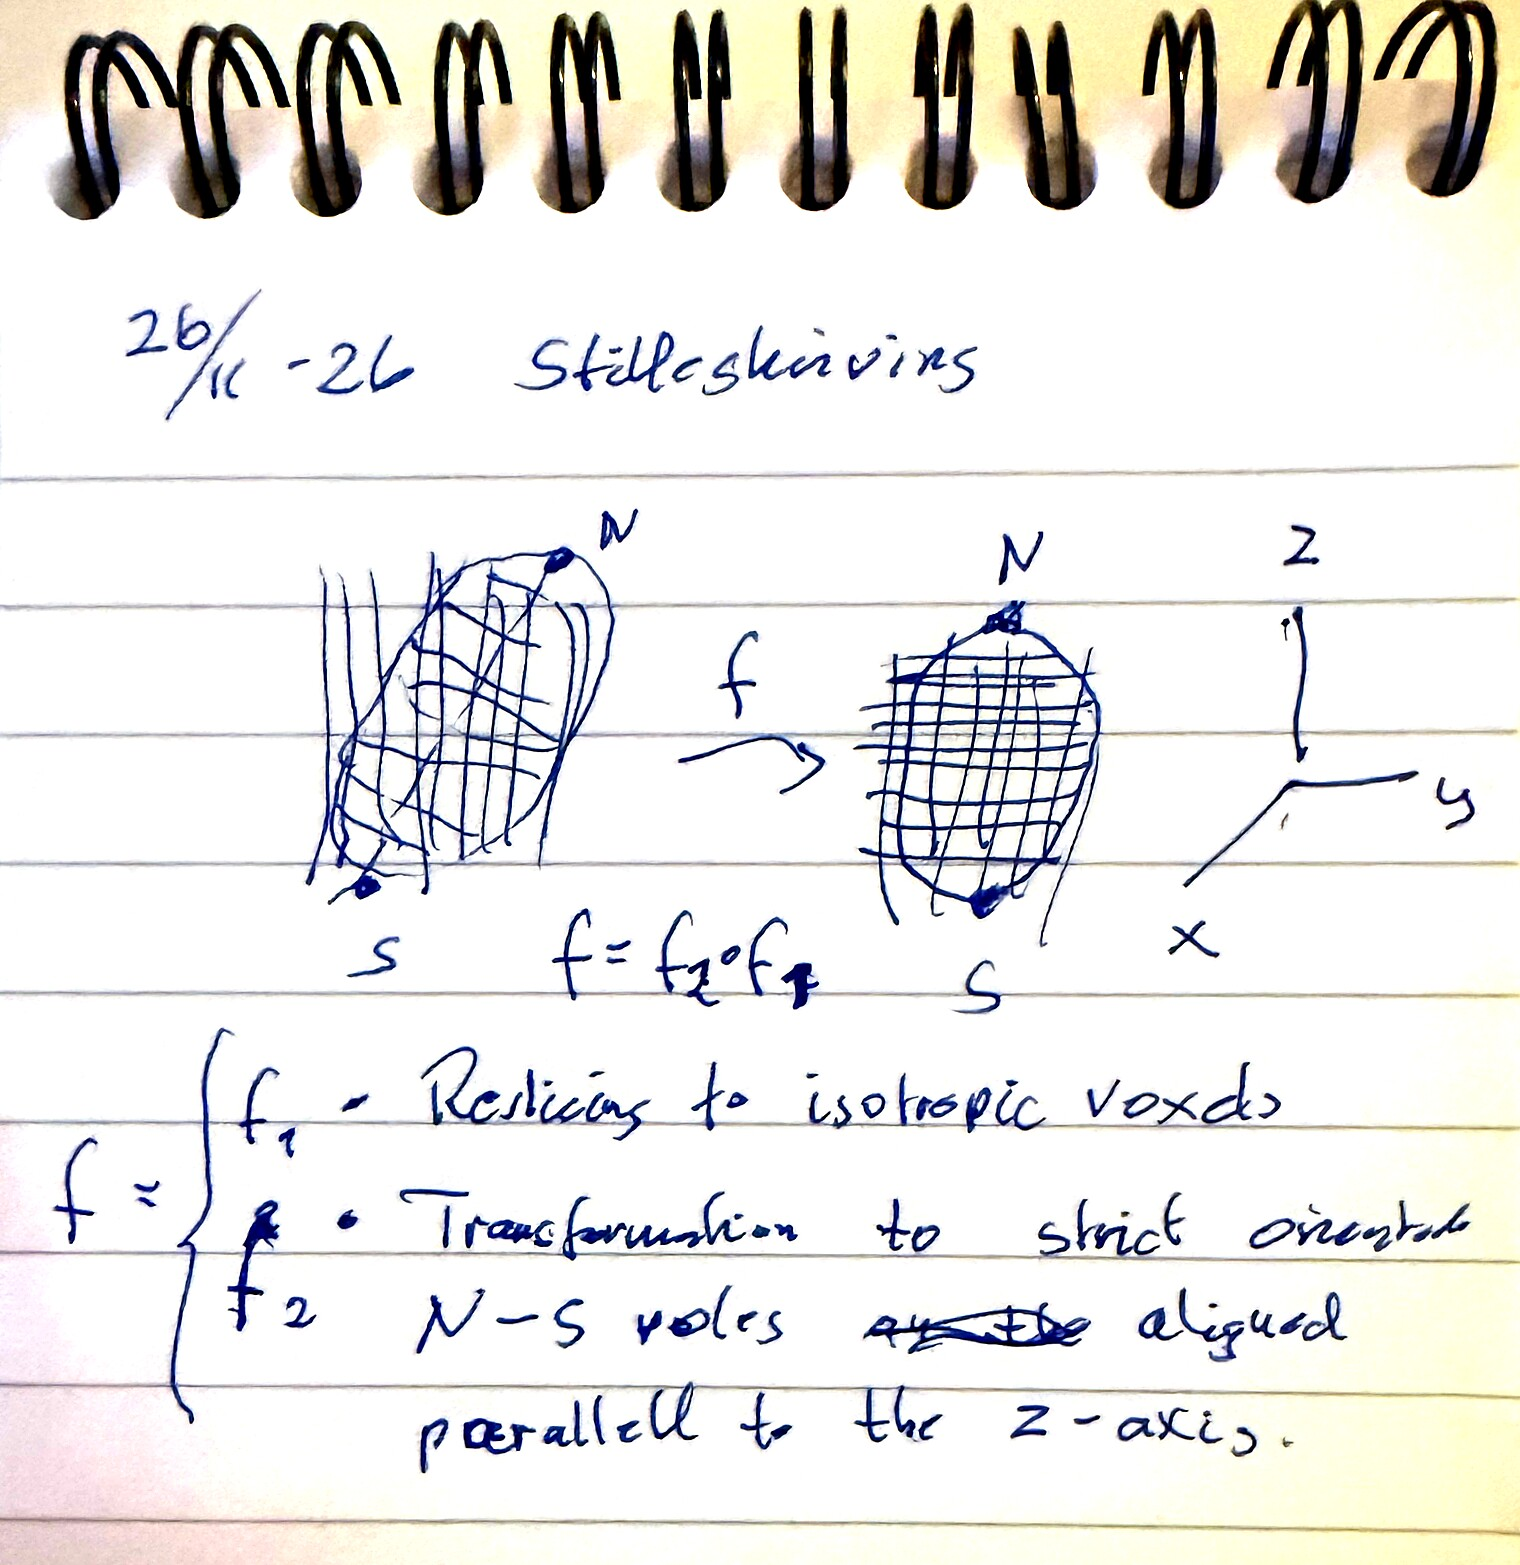
\includegraphics[width=\linewidth]{figures/fig00_sketch_stilleskriving_20261126.jpg}\\[2.5pt]
    {\scriptsize\textit{Original handwritten formulation (26/11-26, Stilleskriving HKS; illumination-enhanced and EXIF-stripped): tilted anisotropic lattice mapped by $f = f_2 \circ f_1$ onto an isotropic cubic grid with N--S poles aligned parallel to the $z$-axis.}\par}
\end{minipage}\hfill
\begin{minipage}[t]{0.61\linewidth}
    \vspace{0pt}
    {\footnotesize\textbf{Original Prompt (reproduced verbatim, 26/11-26):}\\[2.5pt]
    \textit{``In the relation to the Lab4 Kiwi-challenge I wnat to explore the following transformations (being sketched at Stilleskriving HKS 26/11-26 ). This relates to \url{https://github.com/arvidl/BMED365-2027/tree/main/Lab4-Comp-Imag/Kiwi-challenge/docs/neurosymbolic-report/notebooks} and a possible set of initial transformations of the intact 2005 UiB 7\,T Bruker Pharmascan RARE kiwifruit MRI (\texttt{256 $\times$ 256 $\times$ 128}, anisotropic voxel spacing \texttt{0.2344 $\times$ 0.2344 $\times$ 0.5000 mm\textsuperscript{3}}) with implications for the curated 3D Micro-Ground-Truth (\texttt{98} 3D seed instances). The idea behind these intitial transformation is to better deal with the seed segmentation problem (both manual segmentation and automated neurosymbolic segmentation) by making the voxels isotropic obtained by slice interpolation and reslicing along the long axis of the fruit, and then make an affine (rigid) transformation of the Kiwifruit object such that the (estimated) ``North pole'' and ``South pole'' is paralell to the z-axis in the intrisic coordinate system of the kiwi. By proper initial transformations and interpolation techniques - brining the origninal Kiwi recording into a new geometric representation - I thereby expect the manual and automated segmentation problem to be easier to perform and also visualize / evaluate. Eventually, the instance-segmented seeds can also be transformed back to the original Kiwi acquisition. If this is an interesting avenue to explore, please consider an implementation as a new Jupyter notebook 00 in Lab4-Comp-Imag/Kiwi-challenge/docs/neurosymbolic-report/notebooks.''}\par}
\end{minipage}
\end{tcolorbox}
\caption[Multimodal human seed (handwritten sketch and verbatim prompt)]{Authentic multimodal provenance of this study (also embedded in Cell~\texttt{00} of \nbref{00\_isotropic\_reslicing\_and\_polar\_alignment.ipynb}). Preserving the unpolished human prose alongside the spiral-notepad sketch illustrates a core lesson of BMED365: clear physical framing, exact metrological anchors, and falsifiable hypotheses matter far more in AI-assisted scientific coding than polished phrasing.}
\label{fig:sketch_provenance}
\end{figure}

\subsection{Research Questions (\texttt{RQ1}--\texttt{RQ5})}
\label{sec:intro_rqs}

To replace geometric intuition with verifiable quantitative evidence, this technical report investigates five concrete research questions:
\begin{itemize}
    \item \textbf{RQ1 (Intrinsic Polar Axis Discovery):} Among outer-fruit PCA, axial slice-centroid regression, internal columella 3D PCA, and internal columella 3D centerline SVD, which estimator recovers the true botanical North--South polar axis without near-sphericity or 7\,T RF $B_1$ bias, and how much does rigid alignment reduce slice concentricity error?
    \item \textbf{RQ2 (Composite Pullback \& Resolution Trade-Offs):} How much round-trip signal fidelity (PSNR and 3D gradient energy) and compute speed are gained by unifying $f = f_2 \circ f_1$ into a single-pass cubic B-spline homogeneous pullback rather than sequential two-pass trilinear resampling, and how sensitively do tiny $\sim 1\,\text{mm}$ seeds degrade if isotropic spacing $s_{\text{iso}}$ is coarsened from $0.2344\,\text{mm}$ to $0.30\,\text{mm}$ or $0.50\,\text{mm}$?
    \item \textbf{RQ3 (Instance-Label Warping \& Invertibility $f^{-1}\circ f$):} How do Nearest-Neighbor, Per-Instance Soft-Linear, Soft-Cubic, and Index-Space Cubic Signed Distance Field (SDF) operators compare on volume preservation, centroid precision, anti-aliased surface smoothness, and exact round-trip invertibility across all $98$ curated Micro-GT seeds and all $749$ whole-fruit Neurosymbolic predictions?
    \item \textbf{RQ4 (Panoramic Visualization, Manual Curation, \& Seed Orientation):} How does canonical N--S alignment improve manual 3D curation ergonomics (\texttt{freeview}/\texttt{ITK-SNAP}/\texttt{3D Slicer}), straighten carpel columns in cylindrical Mercator atlases $M(\theta', z')$, and expose the intrinsic 3D orientation of seeds relative to radial and polar botanical axes?
    \item \textbf{RQ5 (Controlled Neurosymbolic 3D Learning \& Fair Cross-Grid OOD Safety):} When identical \texttt{AdditiveBayesOrganNet3D} models are trained across $3$ random seeds in Native vs.\ Canonical space and scored on the exact unaltered native $52$-seed test wedge plus unmasked whole-organ OOD volume ($\text{mm}^3$), how does continuous soft pullback $f^{-1}(\hat{p},\hat{d})$ compare against discrete label pullback $f^{-1}(\hat{L})$ and Native training, and what architectural caveats (\texttt{nnU-Net} receptive-field scaling, tilted-prism ROI occupancy) govern production deployment?
\end{itemize}

% =============================================================================
% SECTION 2: MATERIALS AND METHODS
% =============================================================================
\clearpage
\section{Materials and Methods}
\label{sec:methods}

To preserve strict zero-drift synchronization with our Native-space companion report (\natrep{}), all baseline data loaders, neural models (\texttt{AdditiveBayesOrganNet3D}), LTN operators, deep watershed decoders, Mat\'ern steric clump splitters, and Panoptic evaluators are imported untouched from \nbref{kiwi\_ns\_lib.py}, while all new canonical geometric operators ($f_1$, $f_2$, $f = f_2 \circ f_1$, $f^{-1}$, label SDF warpers, Mercator unrolling, and masked tilted-prism training) live in \nbref{00\_isotropic\_reslicing\_and\_polar\_alignment.ipynb}.

\subsection{Archival 7\,T RARE MRI, Bit-Aligned Micro-GT, and Whole-Fruit Predictions}
\label{sec:meth_data}

We operate on three bit-aligned NIfTI-1 volumetric files sharing the exact native lattice $\Omega_{\text{native}}$ ($256 \times 256 \times 128 = 8{,}388{,}608$ voxels), anisotropic voxel spacing $\mathbf{s}_{\text{native}} = (0.234375, 0.234375, 0.500000)\,\text{mm}$ (voxel volume $v_{\text{native}} = 0.027466\,\text{mm}^3$, slice-to-in-plane aspect ratio $2.1333:1$), and identical $4\times 4$ \texttt{sform} affine matrix ($\max|\Delta \mathbf{A}| = 0.000000$):
\begin{equation}
    \begin{bmatrix} x_{\text{mm}} \\ y_{\text{mm}} \\ z_{\text{mm}} \\ 1 \end{bmatrix}
    \;=\;
    \mathbf{A}_{\text{orig}}
    \begin{bmatrix} i \\ j \\ k \\ 1 \end{bmatrix},
    \qquad
    \mathbf{A}_{\text{orig}} \;=\;
    \begin{bmatrix}
        -0.234375 & 0 & 0 & 27.000000 \\
        0 & +0.234375 & 0 & -26.265625 \\
        0 & 0 & +0.500000 & -30.750000 \\
        0 & 0 & 0 & 1
    \end{bmatrix}.
    \label{eq:a_orig}
\end{equation}
The three aligned volumes are: (i)~the raw 7\,T Bruker Pharmascan RARE spin-echo MRI~\cite{hennig1986rare} (\texttt{kiwi\_20050217191129\_131073\_RARE\_high\_res\_axial.nii.gz}, $\text{TE}=63.9\,\text{ms}$, $\text{TR}=18{,}520.8\,\text{ms}$, $\text{ETL}=8$, intact berry volume $85.97\,\text{cm}^3$); (ii)~the curated silver-standard 3D Micro-Ground-Truth (\texttt{kiwi\_micro\_gt\_labels.nii.gz}, \texttt{uint16} instance IDs $1\dots 98$ inside equatorial ROI $x, y \in [128, 208)$, $z \in [56, 72)$, partitioned strictly without voxel overlap at $y_{\text{split}}=168$ into $59$ training seeds and $52$ held-out test seeds); and (iii)~the unmasked 128-slice whole-fruit Neurosymbolic 3D prediction exported by Companion Notebook~\texttt{04} (\texttt{results/kiwi\_neurosymbolic\_pred\_labels.nii.gz}, $749$ discrete 3D seed instances, $0$ polar false positives).

\subsection{End-to-End Bidirectional Canonical Pipeline Architecture}
\label{sec:meth_pipeline}

Figure~\ref{fig:pipeline_arch} summarizes the complete mathematical and operational workflow linking Native Scanner Space $\Omega_{\text{native}}$ and Canonical Isotropic N--S Space $\Omega_{\text{canon}}$, emphasizing that every canonical workflow---manual 3D curation, panoramic atlas QC, or 3D neurosymbolic deep learning---closes the loop through an exact inverse projection $f^{-1}$ back to the unaltered acquisition lattice.

\begin{figure}[htbp]
\centering
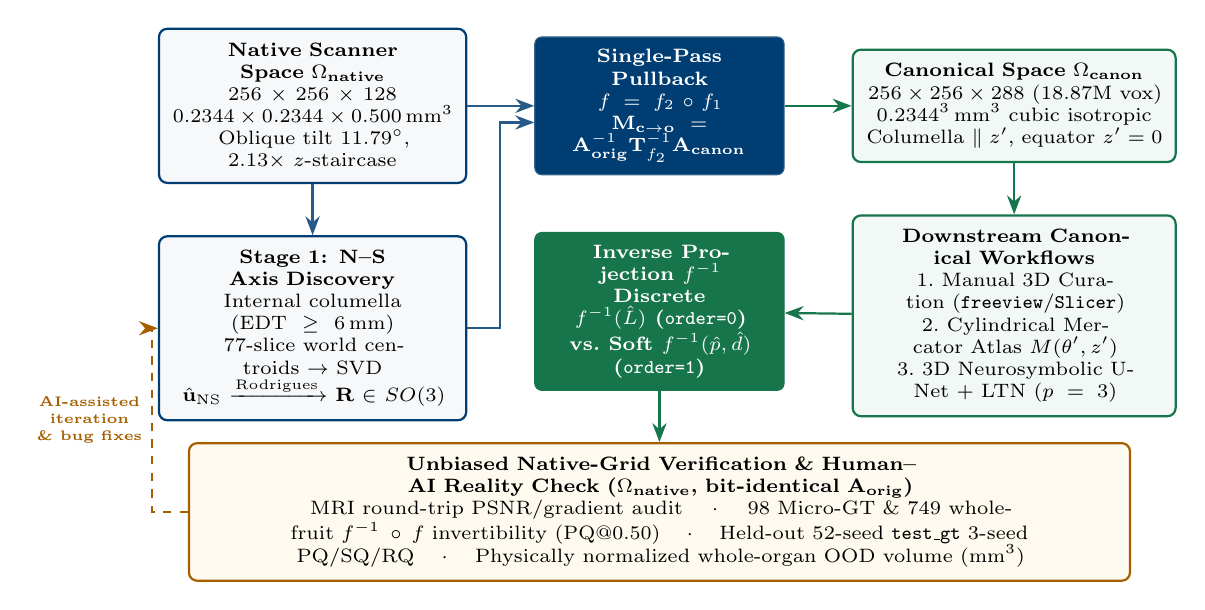
\begin{tikzpicture}[
    node distance=0.55cm and 0.65cm,
    box/.style={rectangle, rounded corners=3pt, draw=uibblue, thick, fill=lightgray, text width=3.55cm, align=center, font=\scriptsize, inner sep=5pt},
    canonbox/.style={rectangle, rounded corners=3pt, draw=kiwigreen!85!black, thick, fill=kiwigreen!6, text width=3.75cm, align=center, font=\scriptsize, inner sep=5pt},
    warnbox/.style={rectangle, rounded corners=3pt, draw=amberwarn, thick, fill=amberbg, text width=3.55cm, align=center, font=\scriptsize, inner sep=5pt},
    opbox/.style={rectangle, rounded corners=2.5pt, draw=uibblue!80, fill=uibblue, text=white, font=\scriptsize\bfseries, align=center, inner sep=4.5pt},
    arrow/.style={-{Stealth[length=2.4mm]}, thick, color=uibblue!85},
    garrow/.style={-{Stealth[length=2.4mm]}, thick, color=kiwigreen!85!black},
    warrow/.style={-{Stealth[length=2.4mm]}, thick, color=amberwarn, dashed}
]
% Row 1: Native -> Pullback -> Canonical
\node[box] (native) {\textbf{Native Scanner Space $\Omega_{\text{native}}$}\\$256\times 256\times 128$\\$0.2344\times 0.2344\times 0.500\,\text{mm}^3$\\Oblique tilt $11.79^\circ$, $2.13\times$ $z$-staircase};

\node[opbox, right=0.85cm of native, text width=2.85cm] (fwd) {Single-Pass Pullback\\$f = f_2 \circ f_1$\\$\mathbf{M}_{\text{c}\to\text{o}} = \mathbf{A}_{\text{orig}}^{-1}\mathbf{T}_{f_2}^{-1}\mathbf{A}_{\text{canon}}$};

\node[canonbox, right=0.85cm of fwd] (canon) {\textbf{Canonical Space $\Omega_{\text{canon}}$}\\$256\times 256\times 288$ ($18.87\text{M}$ vox)\\$0.2344^3\,\text{mm}^3$ cubic isotropic\\Columella $\parallel z'$, equator $z'=0$};

% Sub-block under Native: Columella axis estimation
\node[box, below=0.65cm of native] (axis) {\textbf{Stage 1: N--S Axis Discovery}\\Internal columella ($\text{EDT}\ge 6\,\text{mm}$)\\77-slice world centroids $\to$ SVD\\$\hat{\mathbf{u}}_{\text{NS}} \xrightarrow{\text{Rodrigues}} \mathbf{R}\in SO(3)$};

% Sub-blocks under Canonical: 3 downstream uses
\node[canonbox, below=0.65cm of canon] (uses) {\textbf{Downstream Canonical Workflows}\\1.\ Manual 3D Curation (\texttt{freeview}/\texttt{Slicer})\\2.\ Cylindrical Mercator Atlas $M(\theta',z')$\\3.\ 3D Neurosymbolic U-Net + LTN ($p=3$)};

% Inverse pullback box
\node[opbox, fill=kiwigreen!85!black, draw=kiwigreen!85!black, below=0.72cm of fwd, text width=2.85cm] (inv) {Inverse Projection $f^{-1}$\\Discrete $f^{-1}(\hat{L})$ (\texttt{order=0})\\vs.\ Soft $f^{-1}(\hat{p},\hat{d})$ (\texttt{order=1})};

% Evaluation box
\node[warnbox, below=0.65cm of inv, text width=11.6cm] (eval) {\textbf{Unbiased Native-Grid Verification \& Human--AI Reality Check ($\Omega_{\text{native}}$, bit-identical $\mathbf{A}_{\text{orig}}$)}\\
MRI round-trip PSNR/gradient audit $\;\cdot\;$ 98 Micro-GT \& 749 whole-fruit $f^{-1}\circ f$ invertibility ($\text{PQ@0.50}$) $\;\cdot\;$ Held-out 52-seed \texttt{test\_gt} 3-seed PQ/SQ/RQ $\;\cdot\;$ Physically normalized whole-organ OOD volume ($\text{mm}^3$)};

% Arrows
\draw[arrow] (native) -- (fwd);
\draw[garrow] (fwd) -- (canon);
\draw[arrow] (native) -- (axis);
\draw[arrow] (axis.east) -- ++(0.42,0) |- ([yshift=-6pt]fwd.west);
\draw[garrow] (canon) -- (uses);
\draw[garrow] (uses) -- (inv);
\draw[garrow] (inv) -- (eval);
\draw[warrow] (eval.west) -- ++(-0.45,0) |- node[pos=0.25, left, font=\tiny\bfseries, color=amberwarn, align=center]{AI-assisted\\iteration\\\& bug fixes} (axis.west);
\end{tikzpicture}
\caption[Bidirectional canonical geometric preprocessing architecture ($f$ and $f^{-1}$)]{End-to-end bidirectional canonical representation workflow implemented in Companion Notebook~\texttt{00}. Stage~1 extracts the internal columella centerline to define a minimal-geodesic Rodrigues rotation $\mathbf{R}\in SO(3)$; Stage~2 executes exact single-pass pullback $f = f_2 \circ f_1$ onto $\Omega_{\text{canon}}$; downstream manual, visualization, and neurosymbolic workflows project outputs back via $f^{-1}$ onto unaltered $\Omega_{\text{native}}$ for unbiased metrological auditing.}
\label{fig:pipeline_arch}
\end{figure}

\subsection{Intrinsic North--South Polar Axis Estimation: Four Competing Estimators}
\label{sec:meth_axis}

Before rotating a 3D organ upright, one must answer a deceptively subtle geometric question: \emph{how do we define and measure the organ's intrinsic North--South (N--S) polar axis $\hat{\mathbf{u}}_{\text{NS}}$ directly from 7\,T MRI intensities?} We benchmark four distinct estimators in physical millimeter scanner coordinates $\mathbf{p} = \mathbf{A}_{\text{orig}}\mathbf{i}$ (mathematical derivations and worked examples in Appendix~\ref{app:ellipsoid}):

\begin{enumerate}
    \item \textbf{Estimator~A --- Outer-Fruit Binary Mask 3D PCA ($\hat{\mathbf{u}}_{\text{outer}}$):} Extracts the whole-berry binary mask $M_{\text{fruit}}$ via $\sigma=1.2\,\text{mm}$ Gaussian smoothing, $0.35\times$ Otsu thresholding, slice-wise and 3D hole filling, and largest connected component, then computes the leading eigenvector of its 3D millimeter covariance matrix $\boldsymbol{\Sigma}_{\text{fruit}} = \frac{1}{|M_{\text{fruit}}|}\sum_{\mathbf{p}\in M_{\text{fruit}}}(\mathbf{p}-\bar{\mathbf{p}})(\mathbf{p}-\bar{\mathbf{p}})^\top$.
    \begin{itemize}
        \item \emph{Conceptual pitfall:} Because an intact kiwifruit is nearly spherical (outer-mask principal axis aspect ratio only $1.12:1$), the leading two eigenvalues are nearly degenerate ($\lambda_1 \approx \lambda_2$). Small asymmetric RF $B_1$ signal attenuation near the woody polar caps ($z<11$ and $z>117$) therefore perturbs the principal eigenvector violently, rotating it diagonally \emph{out} of the anatomical core!
    \end{itemize}
    \item \textbf{Estimator~B --- Outer Axial Slice-Centroid Line Regression ($\hat{\mathbf{u}}_{\text{slice}}$):} Computes the 2D outer-fruit centroid $(c_x(z), c_y(z))$ on every populated horizontal slice $z$ and fits a 3D line via linear regression against $z_{\text{mm}}$.
    \begin{itemize}
        \item \emph{Analytical ellipsoid-slicing bias (derived in Appendix~\ref{app:ellipsoid}):} Consider an idealized prolate ellipsoid with semi-axes $(a, b)$ ($a \ge b$) whose major axis is tilted by true angle $\theta$ from the scanner $z$-axis. Slicing it horizontally along $z = \text{const}$ yields 2D elliptical cross-sections whose centroids lie along a line of tilt angle $\alpha_{\text{slice}}$ obeying the exact geometric identity:
        \begin{equation}
            \tan\alpha_{\text{slice}} \;=\; \frac{(a^2 - b^2)\sin\theta\cos\theta}{a^2\cos^2\theta + b^2\sin^2\theta}.
            \label{eq:ellipsoid_bias}
        \end{equation}
        Notice the startling consequence: for a sphere ($a = b$), $\tan\alpha_{\text{slice}} = 0$ regardless of $\theta$! Even for our kiwifruit ($a/b \approx 1.12$, $\theta \approx 11.8^\circ$), Equation~\eqref{eq:ellipsoid_bias} predicts $\alpha_{\text{slice}} \approx 2.6^\circ\text{--}4^\circ \ll 11.8^\circ$---underestimating the true tilt by nearly $3\times$! Worse, this exact mismatch between outer-wall centroid drift ($\approx 4^\circ$) and internal core tilt ($\approx 12^\circ$) creates a systematic \textbf{radial eccentricity error} in native axial slices: as $z$ moves toward either pole, the central columella drifts up to $2.0\,\text{mm}$ ($\approx 8.5$ pixels) away from the outer-fruit centroid used by native \texttt{build\_whole\_organ\_geometry()}.
    \end{itemize}
    \item \textbf{Estimator~C --- Internal Columella 3D PCA ($\hat{\mathbf{u}}_{\text{col,PCA}}$):} Unlike the nearly spherical outer skin, the internal fibrous \emph{columella} is an elongated, deeply hypointense botanical spindle (aspect ratio $3.64:1$) completely enclosed inside bright hydrated locular mucilage and insulated from outer $B_1$ coil edge clipping. We isolate it automatically via: (i)~anisotropic Gaussian smoothing ($\sigma = 0.9\,\text{mm}$); (ii)~interior core gating at least $6.0\,\text{mm}$ inside the skin ($\text{EDT}_{\text{fruit}} \ge 6.0\,\text{mm}$); (iii)~core-zone Otsu thresholding scaled by $0.72$ to capture the dark core cleanly below bright gel; (iv)~3D binary opening ($2$ iterations) to detach touching seeds; and (v)~largest connected component + slice-wise hole filling. Estimator~C takes the leading 3D PCA eigenvector of this columella mask.
    \item \textbf{Estimator~D (Selected) --- Internal Columella 3D Centerline SVD ($\hat{\mathbf{u}}_{\text{NS}}$):} Rather than weighting thick equatorial columella slices disproportionately (as full-volume 3D PCA does), we compute the 2D centroid $\mathbf{q}_k \in \mathbb{R}^3$ (in world millimeters via $\mathbf{A}_{\text{orig}}$) on every axial slice $k$ containing $\ge 250$ columella voxels ($77$ slices spanning the core spindle), center them at $\bar{\mathbf{q}} = \frac{1}{K}\sum_{k=1}^K \mathbf{q}_k$, and extract the total-least-squares principal right singular vector $\hat{\mathbf{u}}_{\text{NS}}$ via Singular Value Decomposition (oriented toward $+z$). Orthogonal residuals $e_k = \|(\mathbf{q}_k - \bar{\mathbf{q}}) - ((\mathbf{q}_k - \bar{\mathbf{q}})\cdot\hat{\mathbf{u}}_{\text{NS}})\hat{\mathbf{u}}_{\text{NS}}\|_2$ directly audit anatomical straightness in millimeters.
\end{enumerate}

\paragraph{Physical pole localization and rigid pivot.}
Projecting the whole-fruit center of mass $\mathbf{p}_{\text{fruit}}$ onto the columella centerline defines the canonical origin pivot $\mathbf{p}_0 = \bar{\mathbf{q}} + \bigl((\mathbf{p}_{\text{fruit}} - \bar{\mathbf{q}})\cdot \hat{\mathbf{u}}_{\text{NS}}\bigr)\hat{\mathbf{u}}_{\text{NS}}$. Tracing the 3D ray $\mathbf{p}(t) = \mathbf{p}_0 + t\,\hat{\mathbf{u}}_{\text{NS}}$ ($t \in [-35, +35]\,\text{mm}$) against $M_{\text{fruit}}$ locates the exact physical \textbf{South Pole} ($\mathbf{p}_{\text{S}} = \mathbf{p}(t_{\text{S}})$) and \textbf{North Pole} ($\mathbf{p}_{\text{N}} = \mathbf{p}(t_{\text{N}})$) surface piercings, giving the intrinsic pole-to-pole fruit length $L_{\text{NS}} = t_{\text{N}} - t_{\text{S}}$.

\subsection{Minimal-Geodesic Rodrigues Alignment ($\mathbf{R} \in SO(3)$) and Canonical Lattice Design}
\label{sec:meth_rodrigues}

Infinitely many 3D rotations map a unit vector $\hat{\mathbf{u}}_{\text{NS}}$ onto $\hat{\mathbf{e}}_z = (0, 0, 1)^\top$, differing by arbitrary azimuthal spin around the $z'$-axis. To preserve the familiar upper-right Micro-GT quadrant orientation of Notebooks~\texttt{01}--\texttt{05} with \textbf{zero extraneous twist}, we construct the unique \textbf{minimal-geodesic Rodrigues rotation} $\mathbf{R} \in SO(3)$ around the axis $\mathbf{v} = \hat{\mathbf{u}}_{\text{NS}} \times \hat{\mathbf{e}}_z$ (full derivation and orthogonality proof in Appendix~\ref{app:so3}):
\begin{equation}
    \mathbf{v} = \hat{\mathbf{u}}_{\text{NS}} \times \hat{\mathbf{e}}_z,\quad
    s = \|\mathbf{v}\|_2,\quad
    c = \hat{\mathbf{u}}_{\text{NS}} \cdot \hat{\mathbf{e}}_z,\qquad
    \mathbf{R} \;=\; \mathbf{I}_3 + [\mathbf{v}]_\times + [\mathbf{v}]_\times^2\,\frac{1 - c}{s^2},
    \label{eq:rodrigues}
\end{equation}
where $[\mathbf{v}]_\times$ is the $3\times 3$ skew-symmetric cross-product matrix satisfying $[\mathbf{v}]_\times \mathbf{w} = \mathbf{v} \times \mathbf{w}$. Combining $\mathbf{R}$ with the translation centering $\mathbf{p}_0$ at the canonical world origin $(0,0,0)$ yields the rigid $4\times 4$ world transformation $\mathbf{T}_{f_2} \in SE(3)$:
\begin{equation}
    \mathbf{T}_{f_2} \;=\; \begin{bmatrix} \mathbf{R} & -\mathbf{R}\mathbf{p}_0 \\ \mathbf{0}^\top & 1 \end{bmatrix},
    \qquad
    \mathbf{p}_{\text{canon}} \;=\; \mathbf{R}\,(\mathbf{p}_{\text{orig}} - \mathbf{p}_0).
    \label{eq:tf2}
\end{equation}

\paragraph{Canonical isotropic grid design ($\Omega_{\text{canon}}$, $\mathbf{A}_{\text{canon}}$).}
We choose canonical cubic spacing $s_{\text{iso}} = 0.234375\,\text{mm}$ (matching native in-plane resolution $1:1$ so zero in-plane seed detail is discarded) and grid dimensions $256 \times 256 \times 288$ ($60.0 \times 60.0 \times 67.5\,\text{mm}^3$ physical field of view, divisible by $16$ along every axis for clean 3D U-Net pooling/upsampling without uneven padding). Preserving the native axis sign convention $\operatorname{diag}(-1, +1, +1)$ so axial/coronal/sagittal viewers display identical anatomical handedness, and mapping the exact grid center index $(127.5, 127.5, 143.5)$ to canonical world $(0, 0, 0)\,\text{mm}$, defines:
\begin{equation}
    \mathbf{A}_{\text{canon}} \;=\;
    \begin{bmatrix}
        -0.234375 & 0 & 0 & +29.8828125 \\
        0 & +0.234375 & 0 & -29.8828125 \\
        0 & 0 & +0.234375 & -33.6328125 \\
        0 & 0 & 0 & 1
    \end{bmatrix}.
    \label{eq:a_canon}
\end{equation}

\subsection{Single-Pass Composite Pullback vs.\ Sequential Resampling and Spacing Audit}
\label{sec:meth_pullback}

\paragraph{Why sequential resampling ($f_1$, then $f_2$) degrades image quality.}
Conceptually, our hypothesis decomposes into two stages: reslice isotropically ($f_1$), then rigidly align ($f_2$). Yet implementing $f_1$ and $f_2$ as \textbf{two sequential discrete interpolation calls} is a classic biomedical signal-processing mistake~\cite{thevenaz2000interpolation,unser1999splines}. Every discrete resampling step convolves the underlying continuous signal with a low-pass interpolation kernel $h(\mathbf{x})$ (frequency response $H(\boldsymbol{\omega})$), compounding attenuation quadratically ($I_{\text{2-pass}} \approx (I * h) * h$, transfer function $|H(\boldsymbol{\omega})|^2$; Appendix~\ref{app:interp}).

\paragraph{Exact single-pass homogeneous backward pullback.}
Because $SE(3)$ and affine lattice maps form a group under $4\times 4$ matrix multiplication, we collapse $f_1$ and $f_2$ into a \textbf{single exact backward pullback matrix} $\mathbf{M}_{\text{canon}\to\text{orig}}$ mapping every target canonical voxel index $\mathbf{i}_{\text{canon}} \in \Omega_{\text{canon}}$ directly to its continuous floating-point coordinate $\mathbf{i}_{\text{orig}} \in \mathbb{R}^3$ inside the unaltered raw scan:
\begin{equation}
    \begin{bmatrix} \mathbf{i}_{\text{orig}} \\ 1 \end{bmatrix}
    \;=\;
    \underbrace{\mathbf{A}_{\text{orig}}^{-1}\,\mathbf{T}_{f_2}^{-1}\,\mathbf{A}_{\text{canon}}}_{\mathbf{M}_{\text{canon}\to\text{orig}}}
    \begin{bmatrix} \mathbf{i}_{\text{canon}} \\ 1 \end{bmatrix},
    \qquad
    \mathbf{M}_{\text{orig}\to\text{canon}} \;=\; \mathbf{M}_{\text{canon}\to\text{orig}}^{-1}
    \;=\; \mathbf{A}_{\text{canon}}^{-1}\,\mathbf{T}_{f_2}\,\mathbf{A}_{\text{orig}}.
    \label{eq:pullback_matrix}
\end{equation}
Backward (pullback) mapping guarantees zero empty holes and zero colliding splats on the target grid. For continuous MRI intensities, we benchmark all four combinations of \textbf{1-Pass Composite vs.\ 2-Pass Sequential} $\times$ \textbf{Trilinear (\texttt{order=1}) vs.\ Cubic B-Spline (\texttt{order=3})} via exact round-trip reconstruction $I_{\text{rt}} = f^{-1}(f(I))$ inside $M_{\text{fruit}}$, measuring: (i)~Root Mean Squared Error ($\text{RMSE}$); (ii)~Peak Signal-to-Noise Ratio $\text{PSNR} = 20\log_{10}(I_{p99}/\text{RMSE})$ ($\text{dB}$); (iii)~3D physical gradient energy retention $\overline{\|\nabla I_{\text{rt}}\|}_2 / \overline{\|\nabla I\|}_2$ (crucial for preserving crisp 1\,mm seed boundaries); (iv)~Gibbs negative undershoot fraction ($\% < 0$, safely clamped at $0.0$ before downstream processing); and (v)~round-trip runtime. We simultaneously audit three isotropic spacings $s_{\text{iso}} \in \{0.2344, 0.3000, 0.5000\}\,\text{mm}$ on grid size, \texttt{float32} RAM, median seed voxel count, MRI PSNR, and 98-seed Micro-GT round-trip $\text{PQ@0.50}$.

\subsection{Instance-Preserving Discrete Label Warping Operators ($f$ and $f^{-1}$)}
\label{sec:meth_labels}

Continuous B-spline interpolation must \textbf{never} be applied directly to a multi-instance integer mask $L : \Omega \to \{0, 1, \dots, K\}$: linearly averaging seed ID~\texttt{\#10} and adjacent seed ID~\texttt{\#20} invents a nonsensical phantom seed~\texttt{\#15}. Instead, we implement and benchmark four mathematically valid instance-preserving label operators (each accelerated via local per-instance bounding-box sub-volumes, running in $0.10\text{--}0.47\,\text{s}$ across all $98$ seeds):
\begin{enumerate}
    \item \textbf{Nearest-Neighbor (\texttt{order=0}):} $\hat{L}(\mathbf{i}') = L[\operatorname{round}(\mathbf{M}\mathbf{i}')]$. Fast, exact integer preservation, minimal volume drift, but carries tilted $0.50\,\text{mm}$ slab staircases into canonical space.
    \item \textbf{Per-Instance Soft-Linear Indicator (\texttt{order=1}, $\tau=0.5$):} For each instance $k$, resample its binary indicator $\mathbf{1}_{L=k}$ trilinearly into $p_k(\mathbf{i}') \in [0, 1]$ and assign $\arg\max_k p_k(\mathbf{i}')$ wherever $\max_k p_k \ge 0.5$. As analyzed in Appendix~\ref{app:interp}, positive mean curvature on tiny $40\text{--}60$-voxel convex seeds causes trilinear averaging to shrink volumes severely ($>10\%$).
    \item \textbf{Per-Instance Soft-Cubic Indicator (\texttt{order=3}, $\tau=0.5$):} Replaces trilinear interpolation of $\mathbf{1}_{L=k}$ with cubic B-spline interpolation prior to $\arg\max_k p_k \ge 0.5$, curbing curvature-driven shrinkage dramatically.
    \item \textbf{Per-Instance Index-Space Cubic Signed Distance Field (SDF, \texttt{order=3}):} Inspired by classical shape-based medical interpolation~\cite{raya1990shapebased}, for each instance $k$ we compute a signed Euclidean Distance Transform in \textbf{symmetric voxel-index coordinates} (positive inside, negative outside):
    \begin{equation}
        \phi_k(\mathbf{i}) \;=\; \operatorname{EDT}_{\text{idx}}(\mathbf{1}_{L=k}) - \operatorname{EDT}_{\text{idx}}(1 - \mathbf{1}_{L=k}),
        \label{eq:index_sdf}
    \end{equation}
    resample $\phi_k$ with cubic B-splines (\texttt{order=3}), and assign $\arg\max_k \phi_k(\mathbf{i}')$ wherever $\max_k \phi_k(\mathbf{i}') > 0$.
    \begin{clinbox}[Critical Geometric Trap Caught During Development: Physical-mm vs.\ Index-Space SDF]
    Computing $\phi_k$ with \emph{anisotropic physical millimeters} $\mathbf{s}=(0.2344, 0.2344, 0.5000)$ biases the zero-crossing inward across top/bottom $z$-caps! Inside a boundary seed voxel, the nearest exterior face along $x$ or $y$ is only $d_{\text{in}} = 0.2344\,\text{mm}$ away, whereas the exterior voxel directly above the $z$-cap sits at $d_{\text{out}} = 0.5000\,\text{mm}$. Interpolating linearly between $+0.2344$ and $-0.5000$ shifts the zero-crossing inward to $0.32$ voxels instead of $0.50$, eroding $z$-caps and shrinking tiny seeds by $\approx 18\%$! Computing $\phi_k$ in \textbf{symmetric index space} ($\Delta i = \Delta j = \Delta k = 1$, where $+1$ inside meets $-1$ outside) locks the zero-crossing exactly halfway at $0.50$ voxels on all six faces (worked proof in Appendix~\ref{app:interp}).
    \end{clinbox}
\end{enumerate}

Every label operator is audited on both forward mapping ($f$: volume error $\Delta V\%$, centroid error in mm against exact analytically rotated centroids $\mathbf{R}(\mathbf{c}_k - \mathbf{p}_0)$) and round-trip invertibility ($f^{-1}\circ f$: 3D Semantic Dice, strict 3D Instance $\text{PQ@0.50}$ via Hungarian matching~\cite{kuhn1955hungarian,kirillov2019panoptic}, surviving seeds out of $98$, and round-trip centroid error), followed by whole-organ $f^{-1}\circ f$ verification across all $749$ whole-fruit Neurosymbolic predictions.

\subsection{Cylindrical Mercator Unrolling, Carpel Slant, and 3D Seed Orientation}
\label{sec:meth_mercator}

In the upright canonical frame $(u', v', z')$ centered on the columella axis ($u'=0, v'=0$), every tissue point admits cylindrical coordinates $r' = \sqrt{u'^2 + v'^2}$, $\theta' = \operatorname{atan2}(v', u') \in [0^\circ, 360^\circ)$, and latitude $z' \in [-L_{\text{NS}}/2, +L_{\text{NS}}/2]$. We construct the canonical $B_1$-invariant $T_2$ contrast ratio $r_{T_2}(\mathbf{x}') = I(\mathbf{x}') / (E_{\text{local}}(\mathbf{x}') + 0.03)$ using a fast separable isotropic $7\times 7\times 7$ grayscale morphological closing ($1.64\,\text{mm}$ window, $2.30\,\text{s}$ total runtime) and project the seed-bearing annular shell $\rho = r'/R'(z') \in [0.28, 0.56]$ onto a flat 2D \textbf{Cylindrical Mercator Atlas} via Minimum Intensity Projection (MinIP):
\begin{equation}
    M(\theta', z') \;=\; \min_{\rho \in [0.28,\, 0.56]} r_{T_2}\!\Bigl(\rho\,R'(z')\cos\theta',\; \rho\,R'(z')\sin\theta',\; z'\Bigr).
    \label{eq:mercator}
\end{equation}
To quantify botanical straightening objectively rather than only visually, we compute the 2D gradient structure tensor across equatorial/mid-latitude strips ($|z'| \le 16\,\text{mm}$) of both the Native and Canonical Mercator atlases and measure the median and RMS \textbf{carpel meridian slant angle} from exact vertical ($\theta' = \text{const}$). Separately, for every canonical Micro-GT seed with $\ge 25$ voxels ($n=93$), we compute the principal eigenvector $\mathbf{v}_1^{(k)}$ of its 3D coordinate inertia tensor to measure its elongation ($\sqrt{\lambda_1/\lambda_2}$) and 3D angular alignment against the horizontal radial ray $\hat{\mathbf{e}}_r$ and the vertical polar axis $\hat{\mathbf{e}}_{z'}$.

\subsection{Controlled 3-Seed + Whole-Organ OOD Neurosymbolic Ablation Protocol}
\label{sec:meth_ablation}

To test \texttt{RQ5} rigorously without evaluation leakage or cross-grid bias, we run a controlled $3$-seed (\texttt{SEEDS = [2027, 2028, 2029]}) head-to-head experiment training the \textbf{exact same \texttt{AdditiveBayesOrganNet3D} architecture} ($\sim 340{,}803$ parameters, 3-level 3D U-Net backbone + un-normalized $+353$-parameter \texttt{Organ-GPS} log-odds head, LTN Product-implication universal quantifier $p=3$, $90$ epochs from scratch with \texttt{AdamW} + Cosine Annealing, leakage-free train-wedge threshold calibration, and Mat\'ern hard-core clump splitting) in Native Anisotropic space versus Canonical Isotropic N--S space, enforcing five strict experimental controls:

\begin{enumerate}
    \item \textbf{Unaltered Native Evaluation Ground Truth ($52$ Held-Out Seeds):} Every model (Native or Canonical) is ultimately evaluated against the \textbf{exact same unaltered native held-out Test Wedge} (\texttt{ds.test\_gt}, $y \in [168, 208)$, $52$ seeds) at the BMED365 benchmark criterion ($\tau_{\text{IoU}} = 0.25$ with exact Hungarian assignment, matching \natrep{}).
    \item \textbf{Masked Supervised Loss Inside the Tilted Legacy Training Prism ($W_{\text{train}}$):} Transforming the axis-aligned native $80\times 40\times 16$ training wedge via $f$ produces an $11.8^\circ$-tilted prism inside a larger axis-aligned canonical bounding box ($92\times 56\times 52$ voxels), occupying only \textbf{$40.7\%$} of the box! To avoid falsely training the remaining $59.3\%$ unlabeled outer padding as background, we warp the binary training-ROI indicator into $W_{\text{train}}$ and strictly mask supervised BCE, Dice, and EDT losses to $W_{\text{train}}$, while still drawing $40$ test-disjoint unlabeled 3D blocks across the full 288-slice canonical fruit for LTN universal regularization.
    \item \textbf{Discrete vs.\ Continuous Soft Inverse Pullback ($f^{-1}$):} When mapping canonical neural predictions back onto $\Omega_{\text{native}}$, we compare two mathematically distinct strategies:
    \begin{itemize}
        \item \emph{Discrete Label Pullback $f^{-1}(\hat{L}_{\text{canon}})$:} Decode discrete 3D seed instances via isotropic watershed + hard-core split inside $\Omega_{\text{canon}}$, then warp integer IDs back onto $\Omega_{\text{native}}$ via \texttt{order=0}.
        \item \emph{Continuous Soft Pullback $f^{-1}(\hat{p}_{\text{canon}}, \hat{d}_{\text{canon}})$:} Warp the continuous predicted foreground probability field $\hat{p}_{\text{canon}}$ and normalized center-distance field $\hat{d}_{\text{canon}}$ back onto $\Omega_{\text{native}}$ via trilinear interpolation (\texttt{order=1}), then perform thresholded 3D watershed + steric split directly on the native grid---avoiding discrete rim quantization and artificial label splits!
    \end{itemize}
    \item \textbf{Physically Normalized Whole-Organ OOD Accounting ($\text{mm}^3$):} Because each canonical voxel ($v_{\text{canon}} = 0.01287\,\text{mm}^3$) is \textbf{$2.133\times$ smaller} than a native voxel ($v_{\text{native}} = 0.02747\,\text{mm}^3$), comparing raw OOD voxel counts across grids would unfairly penalize canonical space by $2.13\times$. We therefore report \textbf{both} physical OOD volume ($\text{mm}^3$) directly in each model's native lattice \emph{and} apples-to-apples native-grid OOD obtained by pulling back the full 288-slice canonical probability volume $f^{-1}(\hat{p}_{\text{wf,canon}})$ onto $\Omega_{\text{native}}$.
    \item \textbf{\texttt{nnU-Net} Spacing--Receptive-Field Control~\cite{isensee2021nnunet}:} Intentionally holding the 3-level \texttt{Backbone3DUNet} architecture fixed while upsampling $z$ by $2.133\times$ halves its physical through-plane receptive field ($\sim 11\,\text{mm} \to \sim 5.2\,\text{mm}$; exact layer calculation in Appendix~\ref{app:mercator_rf}) and roughly doubles training compute ($2.13\times$), isolating the true trade-off between isotropic $3\times 3\times 3$ kernels and physical context span.
\end{enumerate}

\subsection{Human--AI Collaborative Engineering and Verification Methodology}
\label{sec:meth_ai}

Methodologically, this study followed an explicit \textbf{Centaur--Cyborg iterative loop}~\cite{mollick2026coexistence}: human biomedical formulation defined the geometric objective ($f = f_2 \circ f_1$, $f^{-1}$), target specimen, and falsification questions (Figure~\ref{fig:sketch_provenance}); AI coding agents drafted modular NumPy/SciPy/PyTorch prototypes and visual diagnostics; and \textbf{every intermediate output was audited against independent physical invariants} (sagittal/coronal visual overlays, $SO(3)$ orthogonality checks, round-trip PSNR/gradient retention, per-seed volume bias, and cross-grid OOD volume conservation). Whenever an intuitive first implementation failed a physical audit---which happened five distinct times across Sections~1--5---the failure was diagnosed mathematically and retained inside Notebook~\texttt{00} as an explicit didactic ablation rather than silently swept under the rug (detailed in Table~\ref{tab:ai_audit_trail}, Section~\ref{sec:disc_ai}).

% =============================================================================
% SECTION 3: RESULTS
% =============================================================================
\clearpage
\section{Results}
\label{sec:results}

Every quantitative finding below was executed end-to-end in \nbref{00\_isotropic\_reslicing\_and\_polar\_alignment.ipynb} on Apple~Silicon~MPS (\texttt{301.2\,s} total wall-clock runtime) and serialized automatically into \texttt{results/nb00\_canonical\_transform\_audit.json}.

\subsection{Intrinsic Polar Axis Discovery and Slice Concentricity Gains (\texttt{RQ1})}
\label{sec:res_axis}

Table~\ref{tab:axis_estimators} and Figure~\ref{fig:ns_axis} benchmark all four 3D polar-axis estimators head-to-head on the intact 7\,T kiwifruit volume. The empirical discrepancies dramatically confirm both theoretical pitfalls predicted in Section~\ref{sec:meth_axis}:

\begin{table}[htbp]
\centering
\caption[Benchmark of four 3D polar-axis estimators on 7\,T kiwifruit MRI]{Head-to-head quantitative comparison of four 3D polar-axis estimators in physical scanner world coordinates ($\mathbf{A}_{\text{orig}}$). Naive outer-fruit PCA overestimates tilt by $+17.73^\circ$, while horizontal slice-centroid regression underestimates tilt by $-8.05^\circ$ due to near-spherical ellipsoid slicing bias. Source: \texttt{nb00\_canonical\_transform\_audit.json}.}
\label{tab:axis_estimators}
{\footnotesize
\setlength{\tabcolsep}{4pt}
\renewcommand{\arraystretch}{1.24}
\rowcolors{2}{rowalt}{white}
\begin{tabularx}{\textwidth}{L{4.05cm} C{1.35cm} C{1.25cm} C{1.25cm} C{1.45cm} Y}
\toprule
\rowcolor{uibblue!12}\textbf{3D Polar-Axis Estimator} & \textbf{Tilt vs.\ $z$} & \textbf{$X$--$Z$ Tilt} & \textbf{$Y$--$Z$ Tilt} & \textbf{Error vs.\ N--S} & \textbf{Physical Mechanism / Diagnostic Finding} \\
\midrule
Outer-Fruit Binary Mask PCA & $29.25^\circ$ & $-0.30^\circ$ & $+29.25^\circ$ & $17.73^\circ$ & Near-spherical ($1.12:1$) + polar $B_1$ clipping \\
Outer Slice-Centroid Regression & $3.93^\circ$ & $-0.38^\circ$ & $+3.91^\circ$ & $8.05^\circ$ & Underestimated via ellipsoid slicing (Eq.~\ref{eq:ellipsoid_bias}) \\
Internal Columella 3D PCA & $12.85^\circ$ & $+2.17^\circ$ & $+12.67^\circ$ & $1.06^\circ$ & Elongated vascular spindle ($3.64:1$ aspect) \\
\rowcolor{kiwigreen!10}\textbf{Columella 3D Centerline SVD} & $\mathbf{11.79^\circ}$ & $\mathbf{+1.91^\circ}$ & $\mathbf{+11.64^\circ}$ & $\mathbf{0.00^\circ}$ & \textbf{$77$ slices; $0.133\,\text{mm}$ RMS straightness} \\
\bottomrule
\end{tabularx}
}
\end{table}

\begin{figure}[htbp]
    \centering
    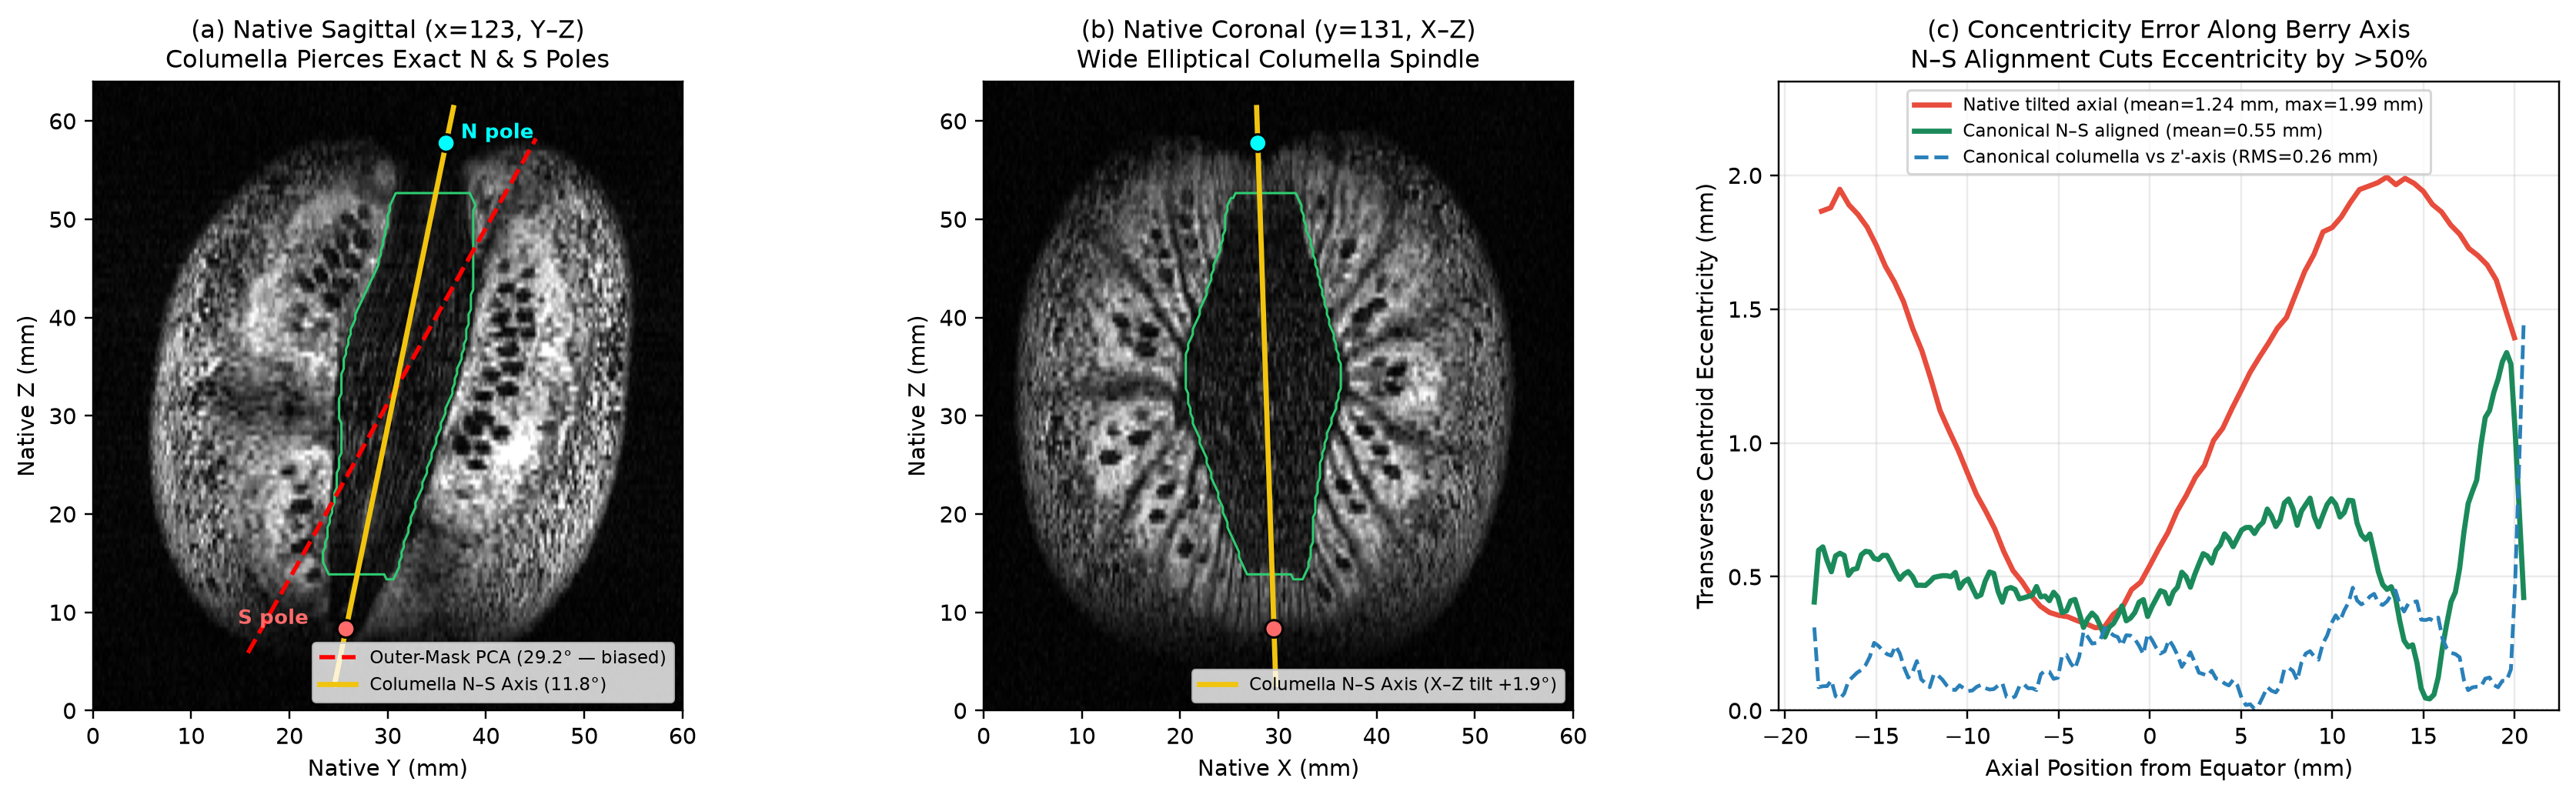
\includegraphics[width=\textwidth]{figures/fig00a_ns_axis_estimation.png}
    \caption[Columella N--S polar axis discovery and slice concentricity error]{\textbf{Intrinsic North--South polar axis discovery and concentricity reduction} (reproduced by Notebook~\texttt{00}, Cell~\texttt{04}). (a)~Native sagittal mid-slice ($x=123$, $Y$--$Z$ plane): naive Outer-Mask PCA (red dashed, $29.2^\circ$) slices diagonally out of the dark central core, whereas the internal Columella 3D Centerline SVD (solid gold, $11.79^\circ$, green segmented contour) tracks the fibrous spindle cleanly and pierces the exact physical South Pole (salmon dot) and North Pole (cyan dot) indentations ($50.50\,\text{mm}$ apart). (b)~Native coronal cross-section ($y=131$, $X$--$Z$ plane) showing the wide elliptical columella spindle and subtle $+1.91^\circ$ $X$--$Z$ lean. (c)~Transverse centroid eccentricity between columella and outer fruit mask along the berry axis: native tilted slices suffer up to $1.99\,\text{mm}$ drift (mean $1.24\,\text{mm}$, red), whereas canonical N--S alignment cuts eccentricity by \textbf{$56.1\%$} (mean $0.55\,\text{mm}$, green) while locking the columella itself onto $(u'=0, v'=0)$ with $0.259\,\text{mm}$ RMS residual (blue dashed).}
    \label{fig:ns_axis}
\end{figure}

\begin{itemize}
    \item \textbf{True botanical N--S orientation:} Across $77$ axial slices, the internal columella centerline is remarkably straight---orthogonal RMS residual is just \textbf{$0.133\,\text{mm}$} (roughly half an in-plane pixel; max residual $0.39\,\text{mm}$)---yielding $\hat{\mathbf{u}}_{\text{NS}} = (0.032583,\; 0.201702,\; 0.978905)^\top$ ($11.79^\circ$ tilt from scanner $z$: $+11.64^\circ$ in $Y$--$Z$ and $+1.91^\circ$ in $X$--$Z$). Piercing the outer fruit surface yields physical poles at $\mathbf{p}_{\text{S}} = (-2.56, -0.50, -22.44)\,\text{mm}$ and $\mathbf{p}_{\text{N}} = (-0.91, +9.68, +27.00)\,\text{mm}$, spanning an exact pole-to-pole length of \textbf{$50.50\,\text{mm}$}.
    \item \textbf{Exact $SO(3)$ orthogonality and concentricity payoff:} Minimal-geodesic Rodrigues rotation $\mathbf{R}$ satisfies $\max|\mathbf{R}^\top\mathbf{R}-\mathbf{I}| = 2.22\times 10^{-16}$ and $\det\mathbf{R} = +1.000000$ (machine epsilon). Transforming into $\Omega_{\text{canon}}$ slashes the transverse eccentricity between the central columella and outer fruit wall by \textbf{$56.1\%$} (mean $1.244 \to 0.546\,\text{mm}$, max $1.994 \to 1.338\,\text{mm}$; Figure~\ref{fig:ns_axis}c), while holding the columella centerline on $(u'=0, v'=0)$ to $0.259\,\text{mm}$ RMS.
\end{itemize}

\subsection{Composite Pullback Fidelity, B-Spline Physics, and Spacing Trade-Off (\texttt{RQ2})}
\label{sec:res_interp}

Tables~\ref{tab:mri_interp}--\ref{tab:spacing_tradeoff} and Figure~\ref{fig:triplanar} report the empirical signal-processing audit of $f = f_2 \circ f_1$ and its inverse $f^{-1}$ on the continuous 7\,T RARE MRI intensities.

\begin{table}[htbp]
\centering
\caption[MRI round-trip interpolation benchmark (1-pass vs.\ 2-pass; trilinear vs.\ cubic B-spline)]{Quantitative round-trip MRI fidelity audit ($f^{-1}(f(I))$ inside $M_{\text{fruit}}$) comparing sequential two-pass resampling ($f_1$ then $f_2$) against single-pass homogeneous pullback ($\mathbf{M}_{\text{canon}\to\text{orig}}$) for trilinear (\texttt{order=1}) and cubic B-spline (\texttt{order=3}) kernels. Source: \texttt{nb00\_canonical\_transform\_audit.json}.}
\label{tab:mri_interp}
{\footnotesize
\setlength{\tabcolsep}{4pt}
\renewcommand{\arraystretch}{1.24}
\rowcolors{2}{rowalt}{white}
\begin{tabularx}{\textwidth}{Y C{1.55cm} C{1.55cm} C{1.75cm} C{1.55cm} C{1.35cm}}
\toprule
\rowcolor{uibblue!12}\textbf{MRI Resampling Strategy ($f^{-1} \circ f$)} & \textbf{RMSE} & \textbf{PSNR (dB)} & \textbf{3D Grad Pres.} & \textbf{Undershoot $<0$} & \textbf{Time (s)} \\
\midrule
2-Pass Sequential ($f_1$ then $f_2$) --- Trilinear (\texttt{order=1}) & $2{,}051.9$ & $20.88$ & $56.23\%$ & $0.000\%$ & $2.18$ \\
1-Pass Composite ($f_2 \circ f_1$) --- Trilinear (\texttt{order=1}) & $1{,}938.1$ & $21.37$ & $59.20\%$ & $0.000\%$ & $0.99$ \\
2-Pass Sequential ($f_1$ then $f_2$) --- Cubic B-Spline (\texttt{order=3}) & $872.6$ & $28.30$ & $90.74\%$ & $0.368\%$ & $10.13$ \\
\rowcolor{kiwigreen!10}\textbf{1-Pass Composite ($f_2 \circ f_1$) --- Cubic B-Spline (Selected)} & $\mathbf{869.7}$ & $\mathbf{28.33}$ & $\mathbf{91.01\%}$ & $\mathbf{0.159\%}$ & $\mathbf{3.87}$ \\
\bottomrule
\end{tabularx}
}
\end{table}

\begin{table}[htbp]
\centering
\caption[Isotropic voxel spacing trade-off audit (0.2344 vs.\ 0.3000 vs.\ 0.5000 mm)]{Isotropic voxel resolution trade-off audit comparing native in-plane preservation ($s_{\text{iso}} = 0.2344\,\text{mm}$), intermediate resampling ($0.30\,\text{mm}$), and slice-thickness coarsening ($0.50\,\text{mm}$) on memory footprint, MRI round-trip PSNR, and 98-seed Micro-GT round-trip Panoptic Quality ($\text{PQ@0.50}$). Source: \texttt{nb00\_canonical\_transform\_audit.json}.}
\label{tab:spacing_tradeoff}
{\footnotesize
\setlength{\tabcolsep}{3.5pt}
\renewcommand{\arraystretch}{1.24}
\rowcolors{2}{rowalt}{white}
\begin{tabularx}{\textwidth}{C{1.75cm} C{2.1cm} C{1.3cm} C{1.35cm} C{1.65cm} C{1.45cm} C{1.45cm} C{1.45cm} Y}
\toprule
\rowcolor{uibblue!12}\textbf{$s_{\text{iso}}$ (mm)} & \textbf{Grid Shape} & \textbf{Voxels} & \textbf{RAM} & \textbf{Med.\ Seed} & \textbf{MRI PSNR} & \textbf{RT Dice} & \textbf{RT PQ@.5} & \textbf{Survived} \\
\midrule
\rowcolor{kiwigreen!10}\textbf{0.2344} & $\mathbf{256{\times}256{\times}288}$ & $\mathbf{18.87\text{M}}$ & $\mathbf{75.5\,\text{MB}}$ & $\mathbf{112\text{ vox}}$ & $\mathbf{28.33\,\text{dB}}$ & $\mathbf{0.9842}$ & $\mathbf{0.9670}$ & $\mathbf{98/98}$ \\
0.3000 & $208{\times}208{\times}240$ & $10.38\text{M}$ & $41.5\,\text{MB}$ & $54\text{ vox}$ & $22.60\,\text{dB}$ & $0.8829$ & $0.7457$ & $95/98$ \\
\rowcolor{amberbg}0.5000 & $128{\times}128{\times}144$ & $2.36\text{M}$ & $9.4\,\text{MB}$ & $12\text{ vox}$ & $17.06\,\text{dB}$ & $0.7208$ & $0.3968$ & \textbf{66/98} \\
\bottomrule
\end{tabularx}
}
\end{table}

\begin{figure}[htbp]
    \centering
    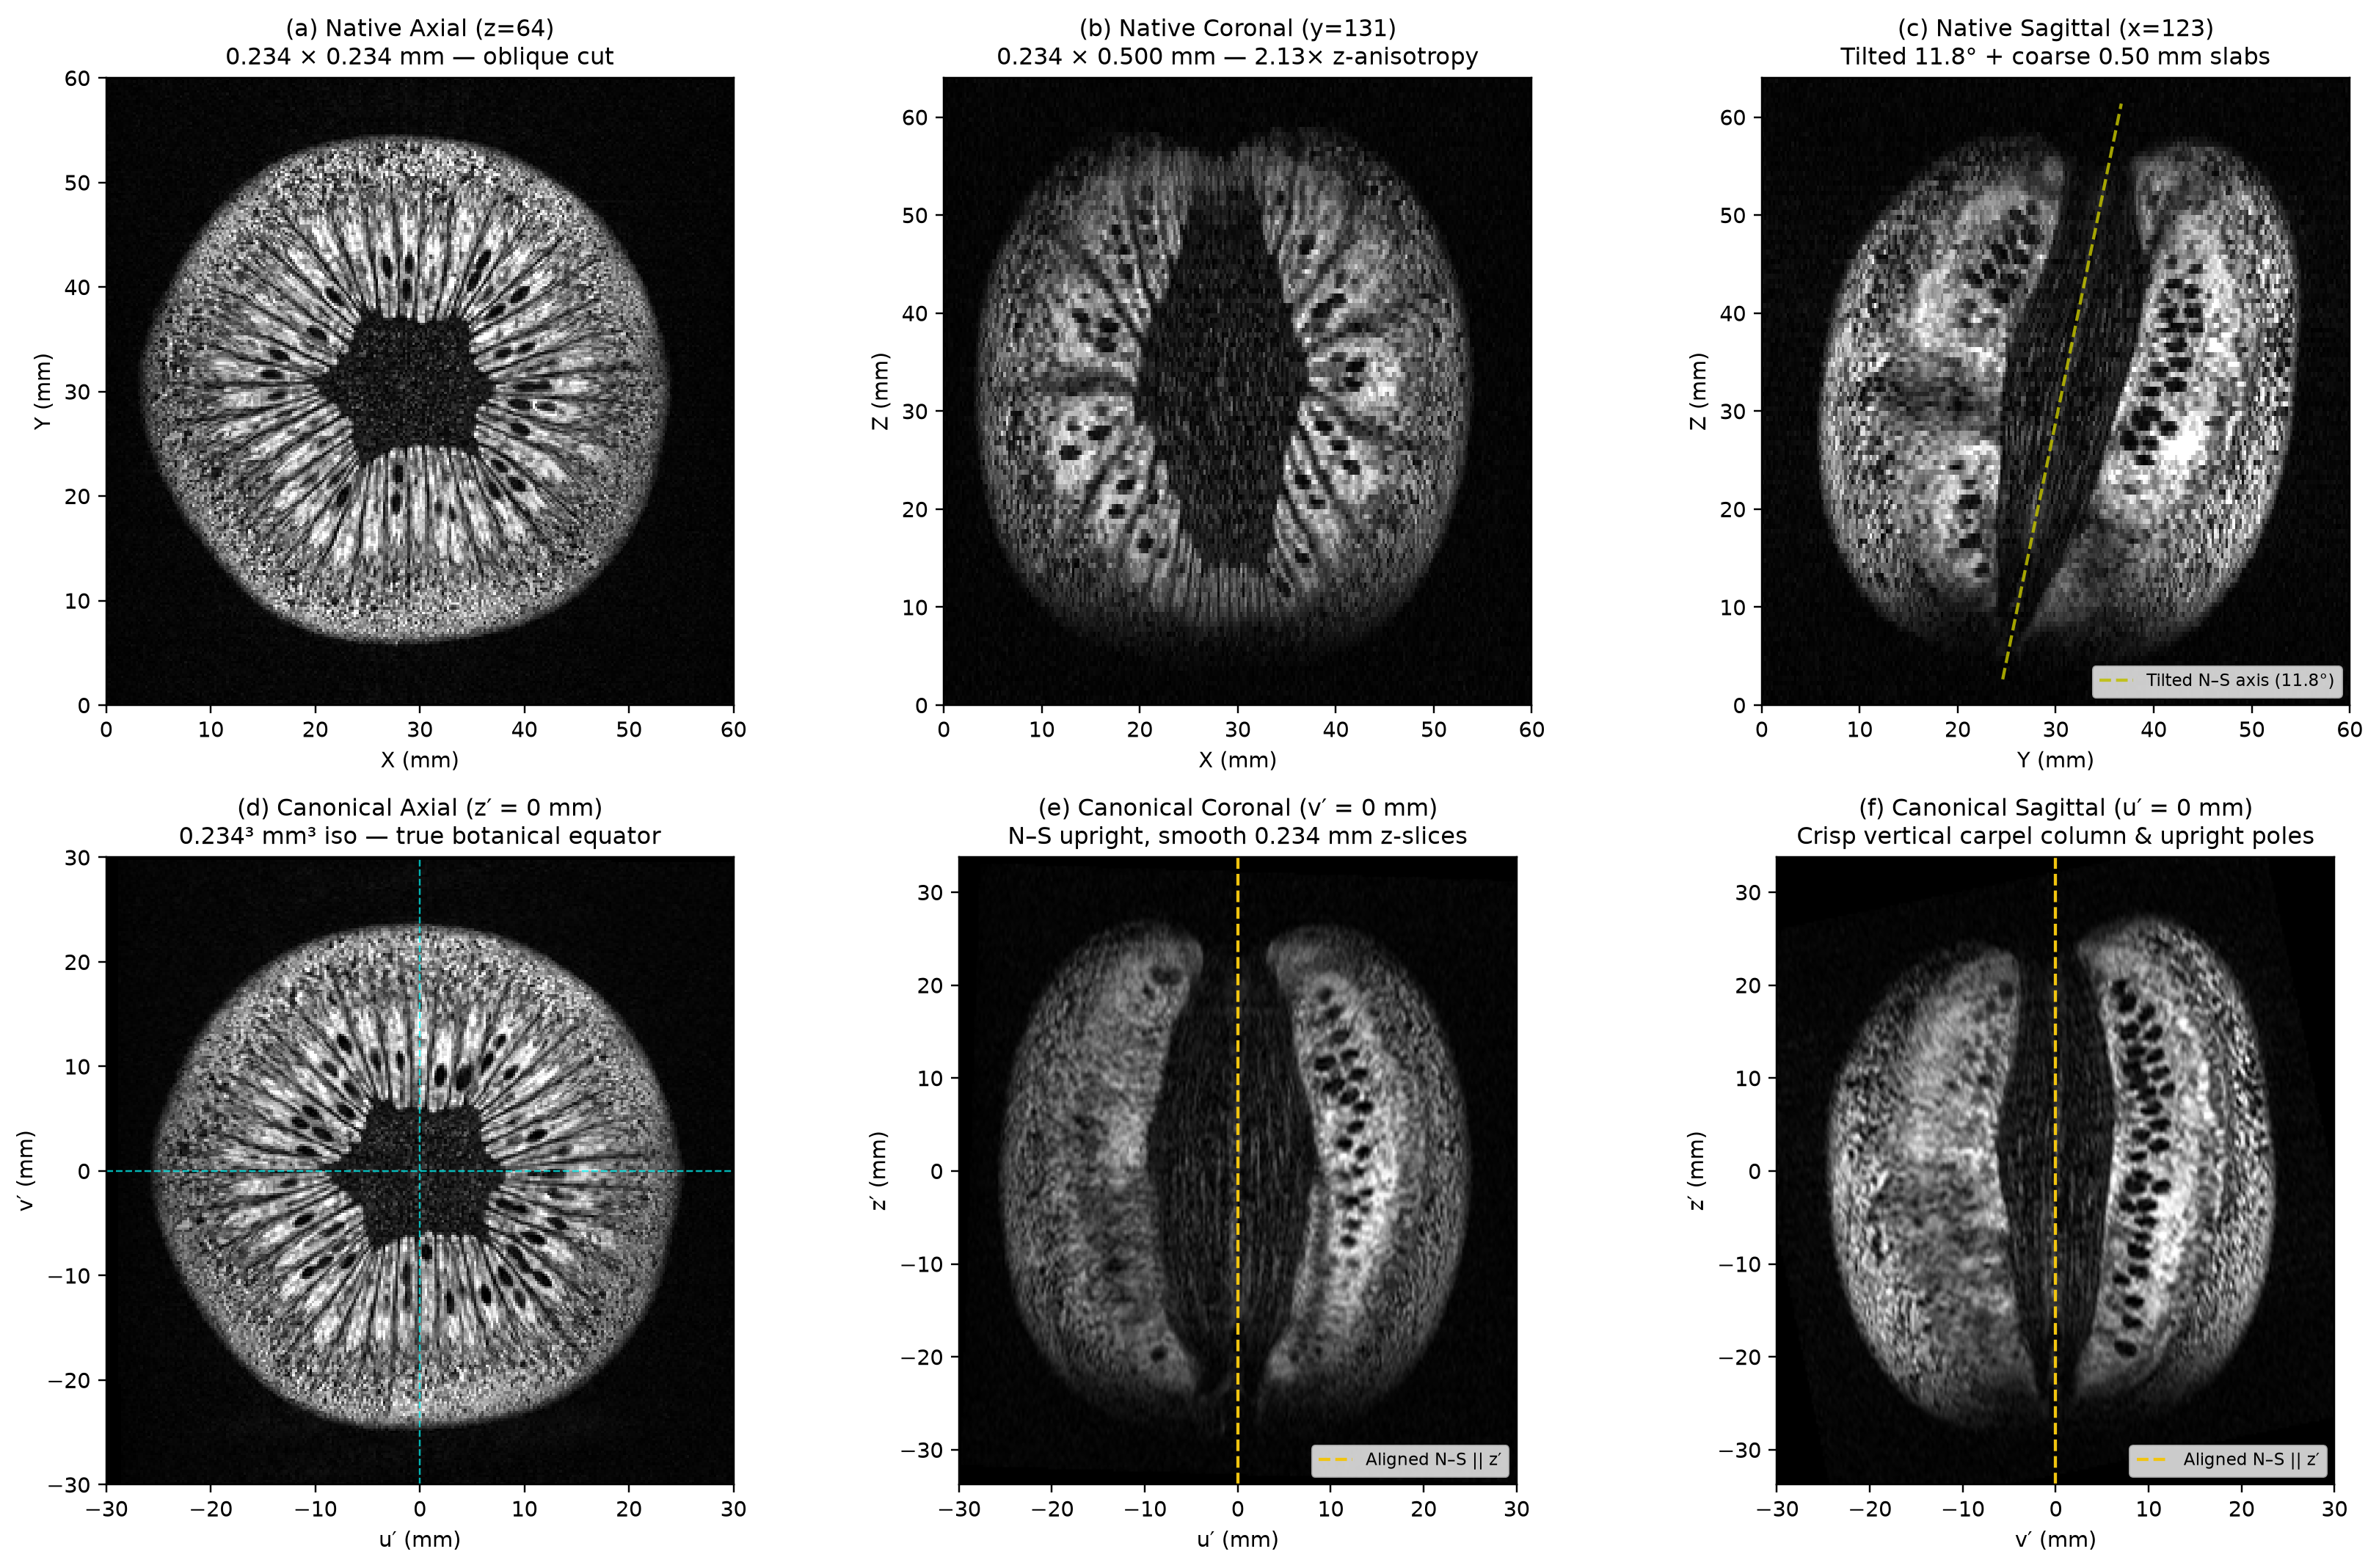
\includegraphics[width=\textwidth]{figures/fig00b_native_vs_canonical_triplanar.png}
    \caption[Native anisotropic tilted vs.\ canonical isotropic N--S aligned tri-planar MRI]{\textbf{Side-by-side tri-planar comparison: Native anisotropic tilted MRI (top) vs.\ Canonical isotropic N--S aligned MRI via single-pass cubic B-spline pullback (bottom)} (reproduced by Notebook~\texttt{00}, Cell~\texttt{06}). Top row (a--c): oblique axial cut ($z=64$), anisotropic coronal ($2.13\times$ $z$-staircasing), and tilted sagittal ($11.8^\circ$ dashed yellow axis + coarse $0.50\,\text{mm}$ slabs). Bottom row (d--f): true botanical equator ($z'=0\,\text{mm}$) centered cleanly on $(u'=0, v'=0)$, upright coronal ($v'=0$), and upright sagittal ($u'=0$) showing razor-sharp vertical carpel columns and upright North/South poles with zero through-plane staircasing.}
    \label{fig:triplanar}
\end{figure}

Three striking quantitative conclusions emerge from Tables~\ref{tab:mri_interp}--\ref{tab:spacing_tradeoff}:
\begin{enumerate}
    \item \textbf{Cubic B-spline pullback crushes trilinear blur by $+7.45\,\text{dB}$:} Naive two-pass trilinear resampling destroys \textbf{$43.8\%$} of 3D physical gradient energy ($56.23\%$ retained; $\text{PSNR} = 20.88\,\text{dB}$), severely washing out thin $1\,\text{mm}$ dark seed rims. Single-pass composite cubic B-spline pullback jumps to \textbf{$28.33\,\text{dB}$ PSNR}, preserves \textbf{$91.01\%$} of 3D gradient energy, halves Gibbs negative undershoot relative to two-pass cubic ($0.159\%$ vs.\ $0.368\%$, safely clamped at $0.0$), and executes \textbf{$2.62\times$ faster} ($3.87\,\text{s}$ vs.\ $10.13\,\text{s}$).
    \item \textbf{Never downsample in-plane resolution to match thick slices:} Coarsening $s_{\text{iso}}$ to $0.50\,\text{mm}$ shrinks RAM to $9.4\,\text{MB}$ but is catastrophic for small biomedical targets: median seed support drops from $112$ voxels to just $12$ voxels, MRI PSNR collapses by $-11.27\,\text{dB}$ ($17.06\,\text{dB}$), and \textbf{$32$ of $98$ seeds fail strict $\text{IoU}\ge 0.50$ recovery} ($\text{PQ@0.50} = 0.3968$). Even $0.30\,\text{mm}$ loses $3$ seeds and drops $\text{PQ@0.50}$ by $-0.221$. Preserving native in-plane resolution ($s_{\text{iso}} = 0.2344\,\text{mm}$, only $75.5\,\text{MB}$ \texttt{float32}, comfortably inside Google Colab's $12\,\text{GB}$ RAM) is strictly mandatory.
    \item \textbf{Visual transformation (Figure~\ref{fig:triplanar}):} In panels~(d)--(f), the dark fibrous columella stands dead vertical along $u'=0, v'=0$, surrounding carpel seed columns run straight vertically from South to North Pole, and through-plane staircasing disappears completely.
\end{enumerate}

\subsection{Instance-Label Warping, $f^{-1}\circ f$ Invertibility, and 3D Seed Morphology (\texttt{RQ3})}
\label{sec:res_labels}

Table~\ref{tab:label_warping} and Figure~\ref{fig:label_warping} quantify all four discrete multi-instance label-warping operators across the $98$ Micro-GT seeds (at strict $\tau_{\text{IoU}} = 0.50$), together with whole-organ invertibility on all $749$ whole-fruit Neurosymbolic predictions.

\begin{table}[htbp]
\centering
\caption[Benchmark of four discrete instance-label warping methods on 98 Micro-GT seeds]{Forward ($f$) and round-trip ($f^{-1}\circ f$) fidelity across four instance-preserving discrete label-warping methods on all $98$ curated Micro-GT seeds (strict $\tau_{\text{IoU}} = 0.50$). Soft-Linear suffers severe $-11.18\%$ curvature-driven shrinkage; Nearest-Neighbor maximizes round-trip reversibility, while Index-Space Cubic SDF yields smooth anti-aliased isotropic surfaces with $+0.60\%$ near-zero volume bias and best forward centroid precision ($0.0313\,\text{mm}$). Source: \texttt{nb00\_canonical\_transform\_audit.json}.}
\label{tab:label_warping}
{\footnotesize
\setlength{\tabcolsep}{3.0pt}
\renewcommand{\arraystretch}{1.24}
\rowcolors{2}{rowalt}{white}
\begin{tabularx}{\textwidth}{Y C{1.35cm} C{1.35cm} C{1.4cm} C{1.15cm} C{1.3cm} C{1.05cm} C{1.4cm} C{0.9cm}}
\toprule
\rowcolor{uibblue!12}\textbf{Label Warping Method} & \textbf{Fwd Med $\Delta V$} & \textbf{Fwd $|\Delta V|$} & \textbf{Fwd Cent.\ (mm)} & \textbf{RT Dice} & \textbf{RT PQ@.5} & \textbf{TP/98} & \textbf{RT Cent.\ (mm)} & \textbf{Time (s)} \\
\midrule
\textbf{Nearest-Neighbor (\texttt{order=0})} & $-0.68\%$ & $\mathbf{2.71\%}$ & $0.0553$ & $\mathbf{0.9842}$ & $\mathbf{0.9670}$ & $\mathbf{98/98}$ & $\mathbf{0.0137}$ & $0.47$ \\
\rowcolor{amberbg}Soft-Linear (\texttt{order=1}) & $\mathbf{-11.18\%}$ & $13.79\%$ & $0.0359$ & $0.9539$ & $0.8832$ & $97/98$ & $0.0435$ & $0.10$ \\
Soft-Cubic (\texttt{order=3}) & $-2.78\%$ & $4.51\%$ & $0.0327$ & $0.9822$ & $0.9537$ & $98/98$ & $0.0193$ & $0.17$ \\
\rowcolor{kiwigreen!10}\textbf{Index-SDF Cubic (\texttt{order=3})} & $\mathbf{+0.60\%}$ & $3.88\%$ & $\mathbf{0.0313}$ & $0.9769$ & $0.9437$ & $\mathbf{98/98}$ & $0.0245$ & $0.21$ \\
\bottomrule
\end{tabularx}
}
\end{table}

\begin{figure}[htbp]
    \centering
    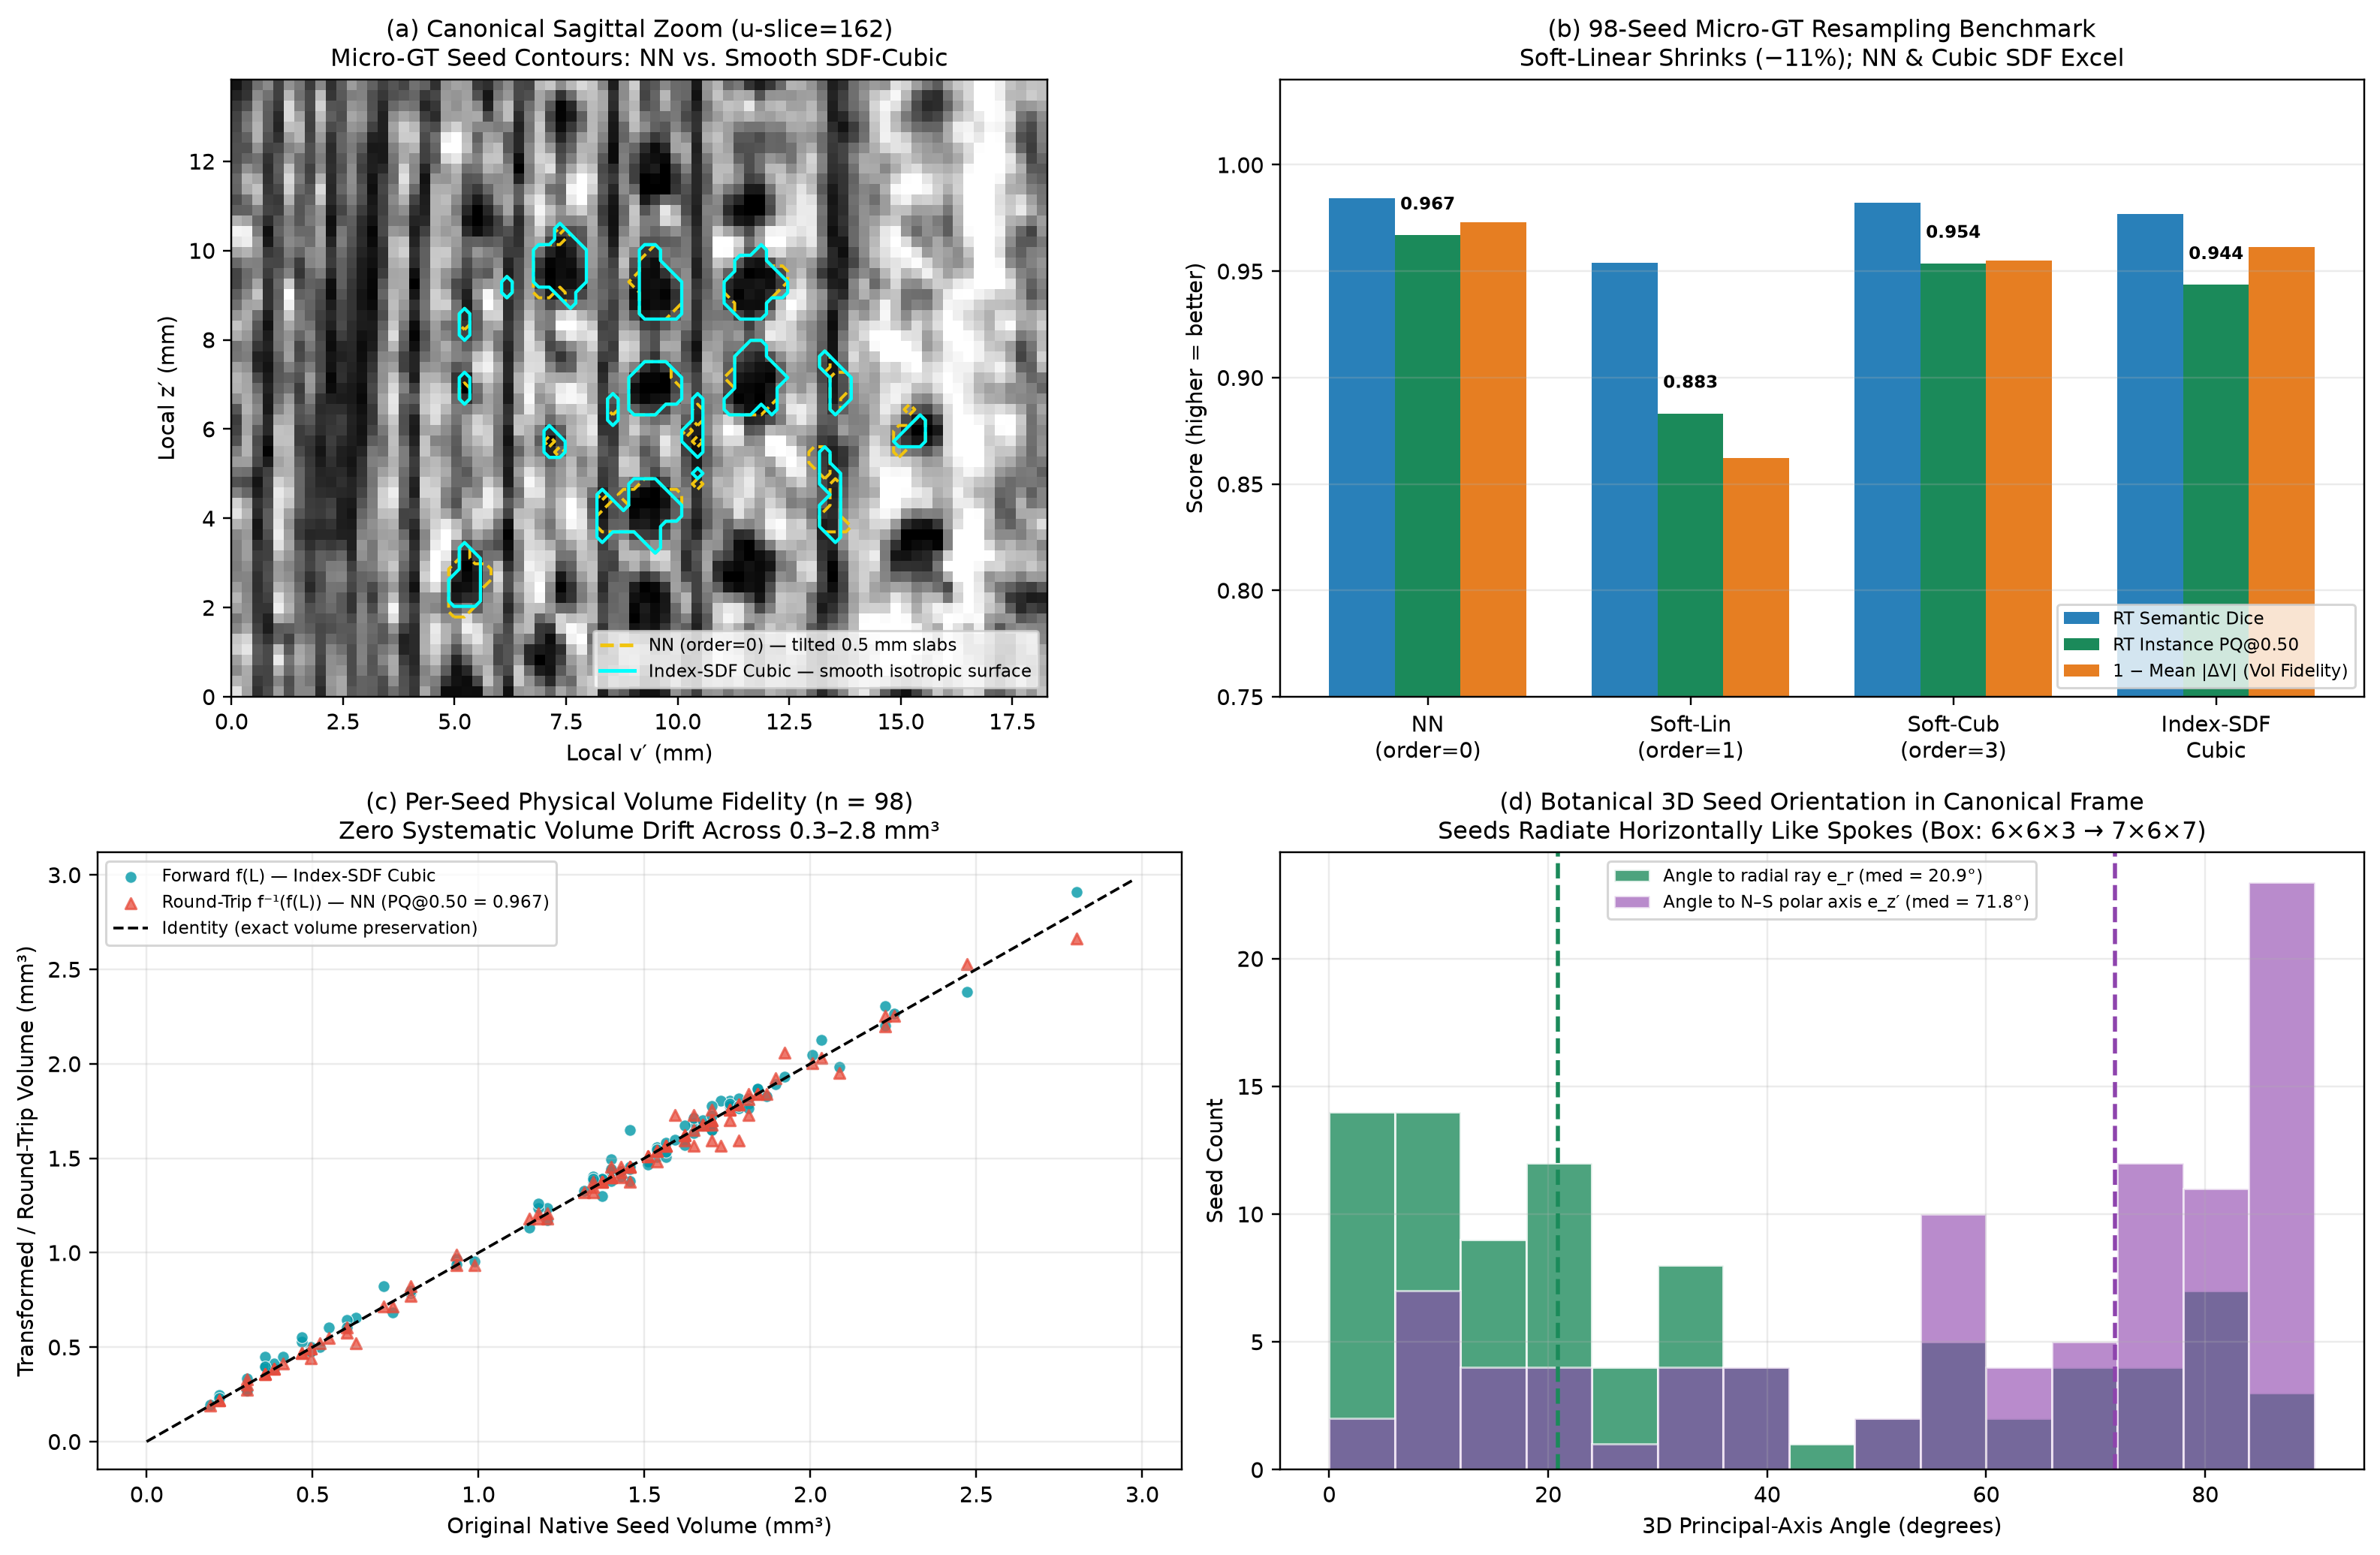
\includegraphics[width=\textwidth]{figures/fig00c_label_interpolation_and_roundtrip.png}
    \caption[98-seed Micro-GT label interpolation benchmark, volume fidelity, and 3D seed orientation]{\textbf{Instance-preserving discrete label resampling, volume fidelity, and botanical 3D seed orientation} (reproduced by Notebook~\texttt{00}, Cell~\texttt{08}). (a)~Canonical sagittal zoom ($u\text{-slice}=162$): Nearest-Neighbor contours (dashed gold) inherit oblique $0.50\,\text{mm}$ staircases, whereas Index-Space Cubic SDF contours (solid cyan) produce smooth, anti-aliased isotropic 3D surfaces aligned to dark seed cores. (b)~98-seed benchmark exposing Soft-Linear's severe volume loss ($-11.18\%$) and lower $\text{PQ@0.50}$ ($0.883$) versus Nearest-Neighbor ($0.967$), Soft-Cubic ($0.954$), and Index-SDF Cubic ($0.944$). (c)~Per-seed physical volume scatter ($n=98$, $0.3\text{--}2.8\,\text{mm}^3$): both forward Index-SDF Cubic (teal dots) and round-trip NN (coral triangles) hug the identity line with zero systematic drift. (d)~Canonical 3D seed principal-axis angles ($n=93$ seeds $\ge 25$ vox): seeds radiate horizontally like bicycle spokes, aligning tightly with transverse radial rays ($\text{median } 20.9^\circ$, green) and roughly orthogonal to the N--S polar axis ($\text{median } 71.8^\circ$, purple).}
    \label{fig:label_warping}
\end{figure}

\begin{itemize}
    \item \textbf{Curvature-driven shrinkage exposed:} Trilinear per-instance indicator interpolation (\texttt{Soft-Linear}) systematically shrank tiny convex seeds by a median of \textbf{$-11.18\%$} (mean $|\Delta V| = 13.79\%$), dropping one small seed on round-trip ($97/98$, $\text{PQ@0.50} = 0.8832$).
    \item \textbf{Task-matched optimal pair:} \textbf{Index-Space Cubic SDF} delivers smooth anti-aliased isotropic seed surfaces (Figure~\ref{fig:label_warping}a), near-zero median volume bias ($+0.60\%$), and the highest forward centroid precision ($0.0313\,\text{mm}$, roughly $1/8$ of an in-plane pixel!) in just $0.21\,\text{s}$---making it the ideal forward operator for visualizing or manually editing Micro-GT templates in canonical space. Meanwhile, \textbf{Nearest-Neighbor (\texttt{order=0})} achieves the tightest discrete round-trip reversibility ($\text{Dice} = 0.9842$, $\text{PQ@0.50} = 0.9670$, $98/98$ seeds, $0.0137\,\text{mm}$ RT centroid error).
    \item \textbf{Whole-organ $749$-seed invertibility ($f^{-1}\circ f$):} Across all $749$ unmasked whole-fruit Neurosymbolic predictions from Notebook~\texttt{04}, round-trip transformation achieves \textbf{$\text{TP} = 749/749$ ($\text{FP}=0$, $\text{FN}=0$, $\text{Merges}=0$, $\text{Splits}=0$)}, $\text{Dice} = 0.9848$, and $\text{PQ@0.50} = \text{SQ} = 0.9677$---proving that full-organ manual or automated canonical segmentations project cleanly back onto the unaltered raw scanner grid without losing, fusing, or splitting a single instance!
    \item \textbf{Isotropic seed geometry and radial spoke law:} In $\Omega_{\text{canon}}$, the median seed voxel bounding box transitions from an anisotropic native \textbf{\texttt{6 $\times$ 6 $\times$ 3}} pancake to a nearly cubic \textbf{\texttt{7 $\times$ 6 $\times$ 7}} block. Principal-axis inertia analysis across $n=93$ canonical seeds reveals striking developmental geometry (Figure~\ref{fig:label_warping}d): seeds are moderately elongated (median $\sqrt{\lambda_1/\lambda_2} = 1.48$) and point radially outward from the columella like spokes, with a median angle of just \textbf{$20.9^\circ$} (IQR $[10.7^\circ, 55.4^\circ]$) to the transverse radial ray $\hat{\mathbf{e}}_r$ and \textbf{$71.8^\circ$} (IQR $[36.7^\circ, 82.8^\circ]$) to the polar axis $\hat{\mathbf{e}}_{z'}$.
\end{itemize}

\subsection{Cylindrical Mercator Atlas and Manual 3D Curation Ergonomics (\texttt{RQ4})}
\label{sec:res_mercator}

Figure~\ref{fig:mercator} contrasts cylindrical MinIP unrolling around the tilted native scanner $z$-axis (panel~a) against our canonically aligned N--S columella axis (panel~b), accompanied by the South-to-North latitude density profile of all $749$ whole-fruit predictions (panel~c).

\begin{figure}[htbp]
    \centering
    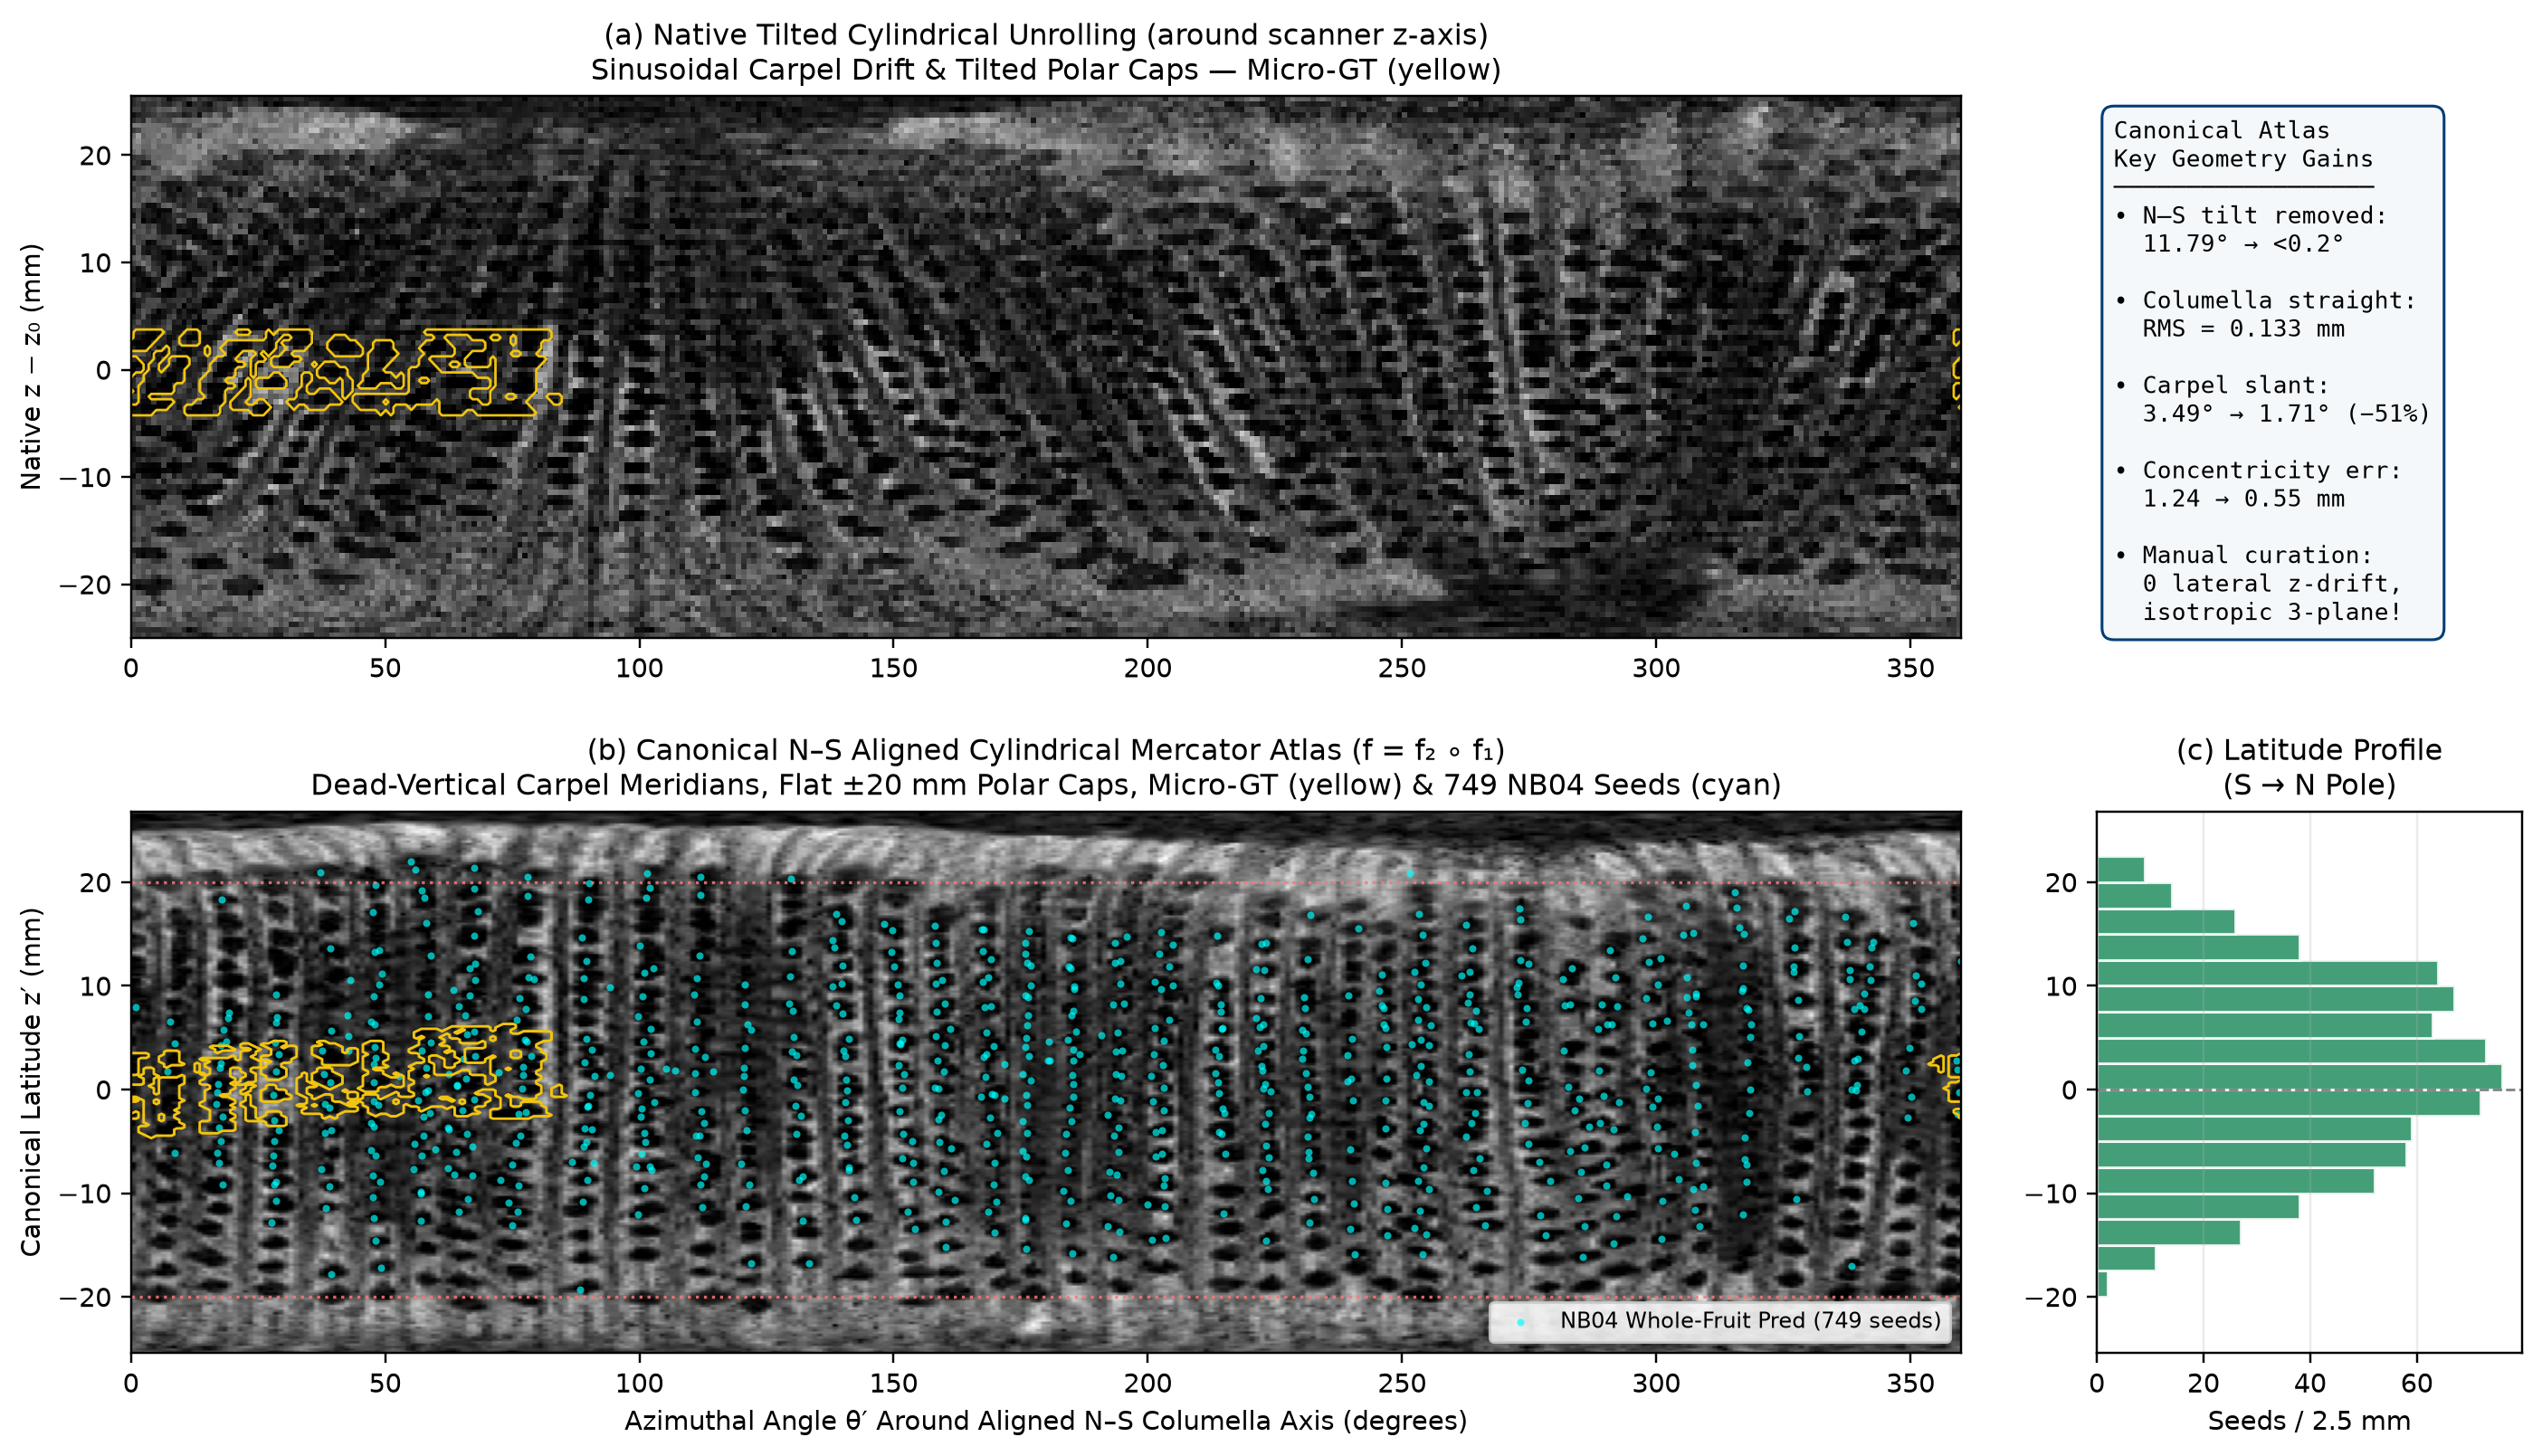
\includegraphics[width=\textwidth]{figures/fig00d_cylindrical_mercator_atlas.png}
    \caption[Native vs.\ canonical cylindrical Mercator botanical atlas]{\textbf{Botanical Cylindrical Mercator Atlas ($M(\theta', z')$): Native tilted unrolling vs.\ Canonical N--S aligned panoramic projection} (reproduced by Notebook~\texttt{00}, Cell~\texttt{10}). (a)~Native cylindrical unrolling around the scanner $z$-axis turns straight botanical carpels into wavy sinusoidal curves (median slant $3.49^\circ$, RMS $4.82^\circ$) and tilts the polar caps by $\pm 5\,\text{mm}$. (b)~Canonical N--S alignment cuts carpel meridian slant by \textbf{$51\%$} (median $1.71^\circ$, RMS $2.84^\circ$), rendering all $\sim 30\text{--}34$ carpel seed columns dead vertical between flat horizontal $\pm 20\,\text{mm}$ polar latitude lines (pink dotted), while simultaneously overlaying the $98$ Micro-GT seeds (yellow contours) and all $749$ whole-fruit NB~\texttt{04} Neurosymbolic predictions (cyan centroids). (c)~South-to-North latitude profile ($2.5\,\text{mm}$ bins) revealing symmetric bell-shaped seed packing peaking near the equator ($z'\approx 0$) and tapering smoothly to zero at $\pm 20\,\text{mm}$.}
    \label{fig:mercator}
\end{figure}

Objectively, canonical N--S alignment cuts carpel meridian slant from vertical by \textbf{$51\%$} (median $3.49^\circ \to 1.71^\circ$, RMS $4.82^\circ \to 2.84^\circ$ across $|z|\le 16\,\text{mm}$). All $749$ unmasked whole-fruit Neurosymbolic predictions span canonical latitudes $z' \in [-19.3, +22.0]\,\text{mm}$ with tight normalized radial depth $r'/R'$ median $0.451$ (IQR $[0.393, 0.503]$), immediately exposing any subtle blind spots across the entire $360^\circ$ circumference in a single 2D panoramic view. For \textbf{manual 3D annotation} in FreeSurfer \texttt{freeview}~\cite{fischl2012freesurfer}, \texttt{ITK-SNAP}~\cite{yushkevich2006itksnap}, or \texttt{3D Slicer}~\cite{fedorov2012slicer}, canonical space eliminates all three traditional manual-tracing headaches simultaneously: (i)~zero lateral drift while scrolling axial slices along $z'$, (ii)~crisp isotropic $0.234\,\text{mm}$ coronal and sagittal cross-sections without $0.50\,\text{mm}$ slabs, and (iii)~exact round-trip export back to $\Omega_{\text{native}}$ via $f^{-1}$.

\subsection{Controlled 3-Seed + Whole-Organ OOD Canonical Neurosymbolic Ablation (\texttt{RQ5})}
\label{sec:res_ablation}

Tables~\ref{tab:ablation_3seed}--\ref{tab:ablation_perseed} and Figure~\ref{fig:ablation_canonical} report our controlled $3$-seed (\texttt{2027, 2028, 2029}) comparison of \texttt{AdditiveBayesOrganNet3D} in Native Anisotropic vs.\ Canonical Isotropic N--S space, evaluated strictly on the unaltered native $52$-seed held-out test wedge plus unmasked whole-organ OOD volume ($\text{mm}^3$).

\begin{table}[htbp]
\centering
\caption[3-seed held-out native test wedge \& whole-organ OOD ablation summary]{Controlled 3-seed (\texttt{2027--2029}, 90 epochs, Mean $\pm$ SD) neurosymbolic ablation scored identically on the unaltered native 52-seed test wedge ($\tau_{\text{IoU}} = 0.25$) plus physically normalized unmasked whole-organ OOD volumes ($\text{mm}^3$). Reference NB~\texttt{03} pure-neural Baseline U-Net suffers $5{,}602\,\text{mm}^3$ total OOD ($598\,\text{mm}^3$ polar). Source: \texttt{nb00\_canonical\_transform\_audit.json}.}
\label{tab:ablation_3seed}
{\scriptsize
\setlength{\tabcolsep}{2.6pt}
\renewcommand{\arraystretch}{1.26}
\rowcolors{2}{rowalt}{white}
\begin{tabularx}{\textwidth}{Y C{1.3cm} C{1.3cm} C{1.3cm} C{1.3cm} C{1.3cm} C{1.3cm} C{1.35cm} C{1.35cm} C{1.15cm} C{0.9cm}}
\toprule
\rowcolor{uibblue!12}\textbf{Pipeline (3-Seed Mean $\pm$ SD)} & \textbf{Dice} & \textbf{Prec} & \textbf{Rec} & \textbf{SQ} & \textbf{RQ} & \textbf{PQ} & \textbf{Polar ($\text{mm}^3$)} & \textbf{OOD ($\text{mm}^3$)} & \textbf{$N_{\text{wf}}$} & \textbf{Time} \\
\midrule
Native Anisotropic ($0.234{\times}0.234{\times}0.50$) & $0.674$ $\pm 0.013$ & $0.835$ $\pm 0.041$ & $0.545$ $\pm 0.024$ & $\mathbf{0.691}$ $\pm 0.011$ & $0.659$ $\pm 0.022$ & $0.455$ $\pm 0.013$ & $\mathbf{0.00}$ $\pm 0.00$ & $\mathbf{15.3}$ $\pm 9.7$ & $961$ $\pm 126$ & $\mathbf{22.9\,\text{s}}$ \\
Canonical $\to$ Discrete $f^{-1}(\hat{L})$ & $0.658$ $\pm 0.011$ & $0.821$ $\pm 0.033$ & $\mathbf{0.615}$ $\pm 0.016$ & $0.611$ $\pm 0.013$ & $\mathbf{0.703}$ $\pm 0.022$ & $0.430$ $\pm 0.022$ & $5.66$ $\pm 8.01$ & $49.5$ $\pm 43.7$ & $488$ $\pm 63$ & $48.7\,\text{s}$ \\
\rowcolor{kiwigreen!10}\textbf{Canonical $\to$ Soft $f^{-1}(\hat{p},\hat{d})$} & $\mathbf{0.681}$ $\pm 0.017$ & $\mathbf{0.867}$ $\pm 0.024$ & $0.583$ $\pm 0.009$ & $0.662$ $\pm 0.036$ & $0.697$ $\pm 0.013$ & $\mathbf{0.462}$ $\pm 0.030$ & $4.23$ $\pm 5.77$ & $44.5$ $\pm 41.7$ & $488$ $\pm 63$ & $48.7\,\text{s}$ \\
\bottomrule
\end{tabularx}
}
\end{table}

\begin{table}[htbp]
\centering
\caption[Full per-seed (2027, 2028, 2029) breakdown of Native vs.\ Canonical Discrete vs.\ Canonical Soft pullback]{Complete per-seed breakdown (\texttt{2027}, \texttt{2028}, \texttt{2029}) of held-out native 52-seed test metrics, merge/split error taxonomy, and physically normalized whole-organ OOD safety. Continuous soft pullback $f^{-1}(\hat{p},\hat{d})$ eliminates discrete rim splits ($3, 2 \to 0, 0$ on Seeds 2027--2028) and reaches peak $\text{PQ} = 0.4907$ on Seed 2027. Source: \texttt{nb00\_canonical\_transform\_audit.json}.}
\label{tab:ablation_perseed}
{\scriptsize
\setlength{\tabcolsep}{3.0pt}
\renewcommand{\arraystretch}{1.22}
\rowcolors{2}{rowalt}{white}
\begin{tabularx}{\textwidth}{L{3.55cm} C{0.75cm} C{0.75cm} C{0.85cm} C{0.85cm} C{0.85cm} C{0.9cm} C{0.9cm} C{1.05cm} C{1.15cm} C{1.2cm} Y}
\toprule
\rowcolor{uibblue!12}\textbf{Pipeline} & \textbf{Seed} & \textbf{$\tau^*$} & \textbf{TP/52} & \textbf{FP} & \textbf{M / S} & \textbf{Dice} & \textbf{SQ} & \textbf{PQ} & \textbf{Polar} & \textbf{OOD} & \textbf{$N_{\text{wf}}$} \\
\midrule
Native Anisotropic & 2027 & 0.28 & 30 & 5 & 2 / 0 & 0.6834 & 0.6790 & 0.4683 & 0.00 & 28.84 & 1,104 \\
Native Anisotropic & 2028 & 0.40 & 27 & 4 & 2 / 0 & 0.6828 & 0.7061 & 0.4594 & 0.00 & 6.62 & 798 \\
Native Anisotropic & 2029 & 0.28 & 28 & 8 & 1 / 0 & 0.6551 & 0.6885 & 0.4381 & 0.00 & 10.33 & 982 \\
\midrule
Canonical Discrete $f^{-1}(\hat{L})$ & 2027 & 0.46 & 33 & 6 & 3 / 3 & 0.6698 & 0.6238 & 0.4524 & 0.00 & 15.95 & 463 \\
Canonical Discrete $f^{-1}(\hat{L})$ & 2028 & 0.46 & 32 & 6 & 3 / 2 & 0.6612 & 0.6164 & 0.4384 & 0.00 & 21.35 & 427 \\
Canonical Discrete $f^{-1}(\hat{L})$ & 2029 & 0.34 & 31 & 9 & 4 / 4 & 0.6423 & 0.5940 & 0.4003 & 16.99 & 111.29 & 575 \\
\midrule
\rowcolor{kiwigreen!10}\textbf{Canonical Soft $f^{-1}(\hat{p},\hat{d})$} & \textbf{2027} & \textbf{0.46} & \textbf{30} & \textbf{4} & \textbf{3 / 0} & \textbf{0.7007} & \textbf{0.7034} & \textbf{0.4907} & \textbf{0.30} & \textbf{11.32} & \textbf{463} \\
\rowcolor{kiwigreen!10}\textbf{Canonical Soft $f^{-1}(\hat{p},\hat{d})$} & \textbf{2028} & \textbf{0.46} & \textbf{31} & \textbf{4} & \textbf{4 / 0} & \textbf{0.6820} & \textbf{0.6673} & \textbf{0.4756} & \textbf{0.00} & \textbf{18.76} & \textbf{427} \\
Canonical Soft $f^{-1}(\hat{p},\hat{d})$ & 2029 & 0.34 & 30 & 6 & 4 / 2 & 0.6588 & 0.6161 & 0.4201 & 12.39 & 103.27 & 575 \\
\bottomrule
\end{tabularx}
}
\end{table}

\begin{figure}[htbp]
    \centering
    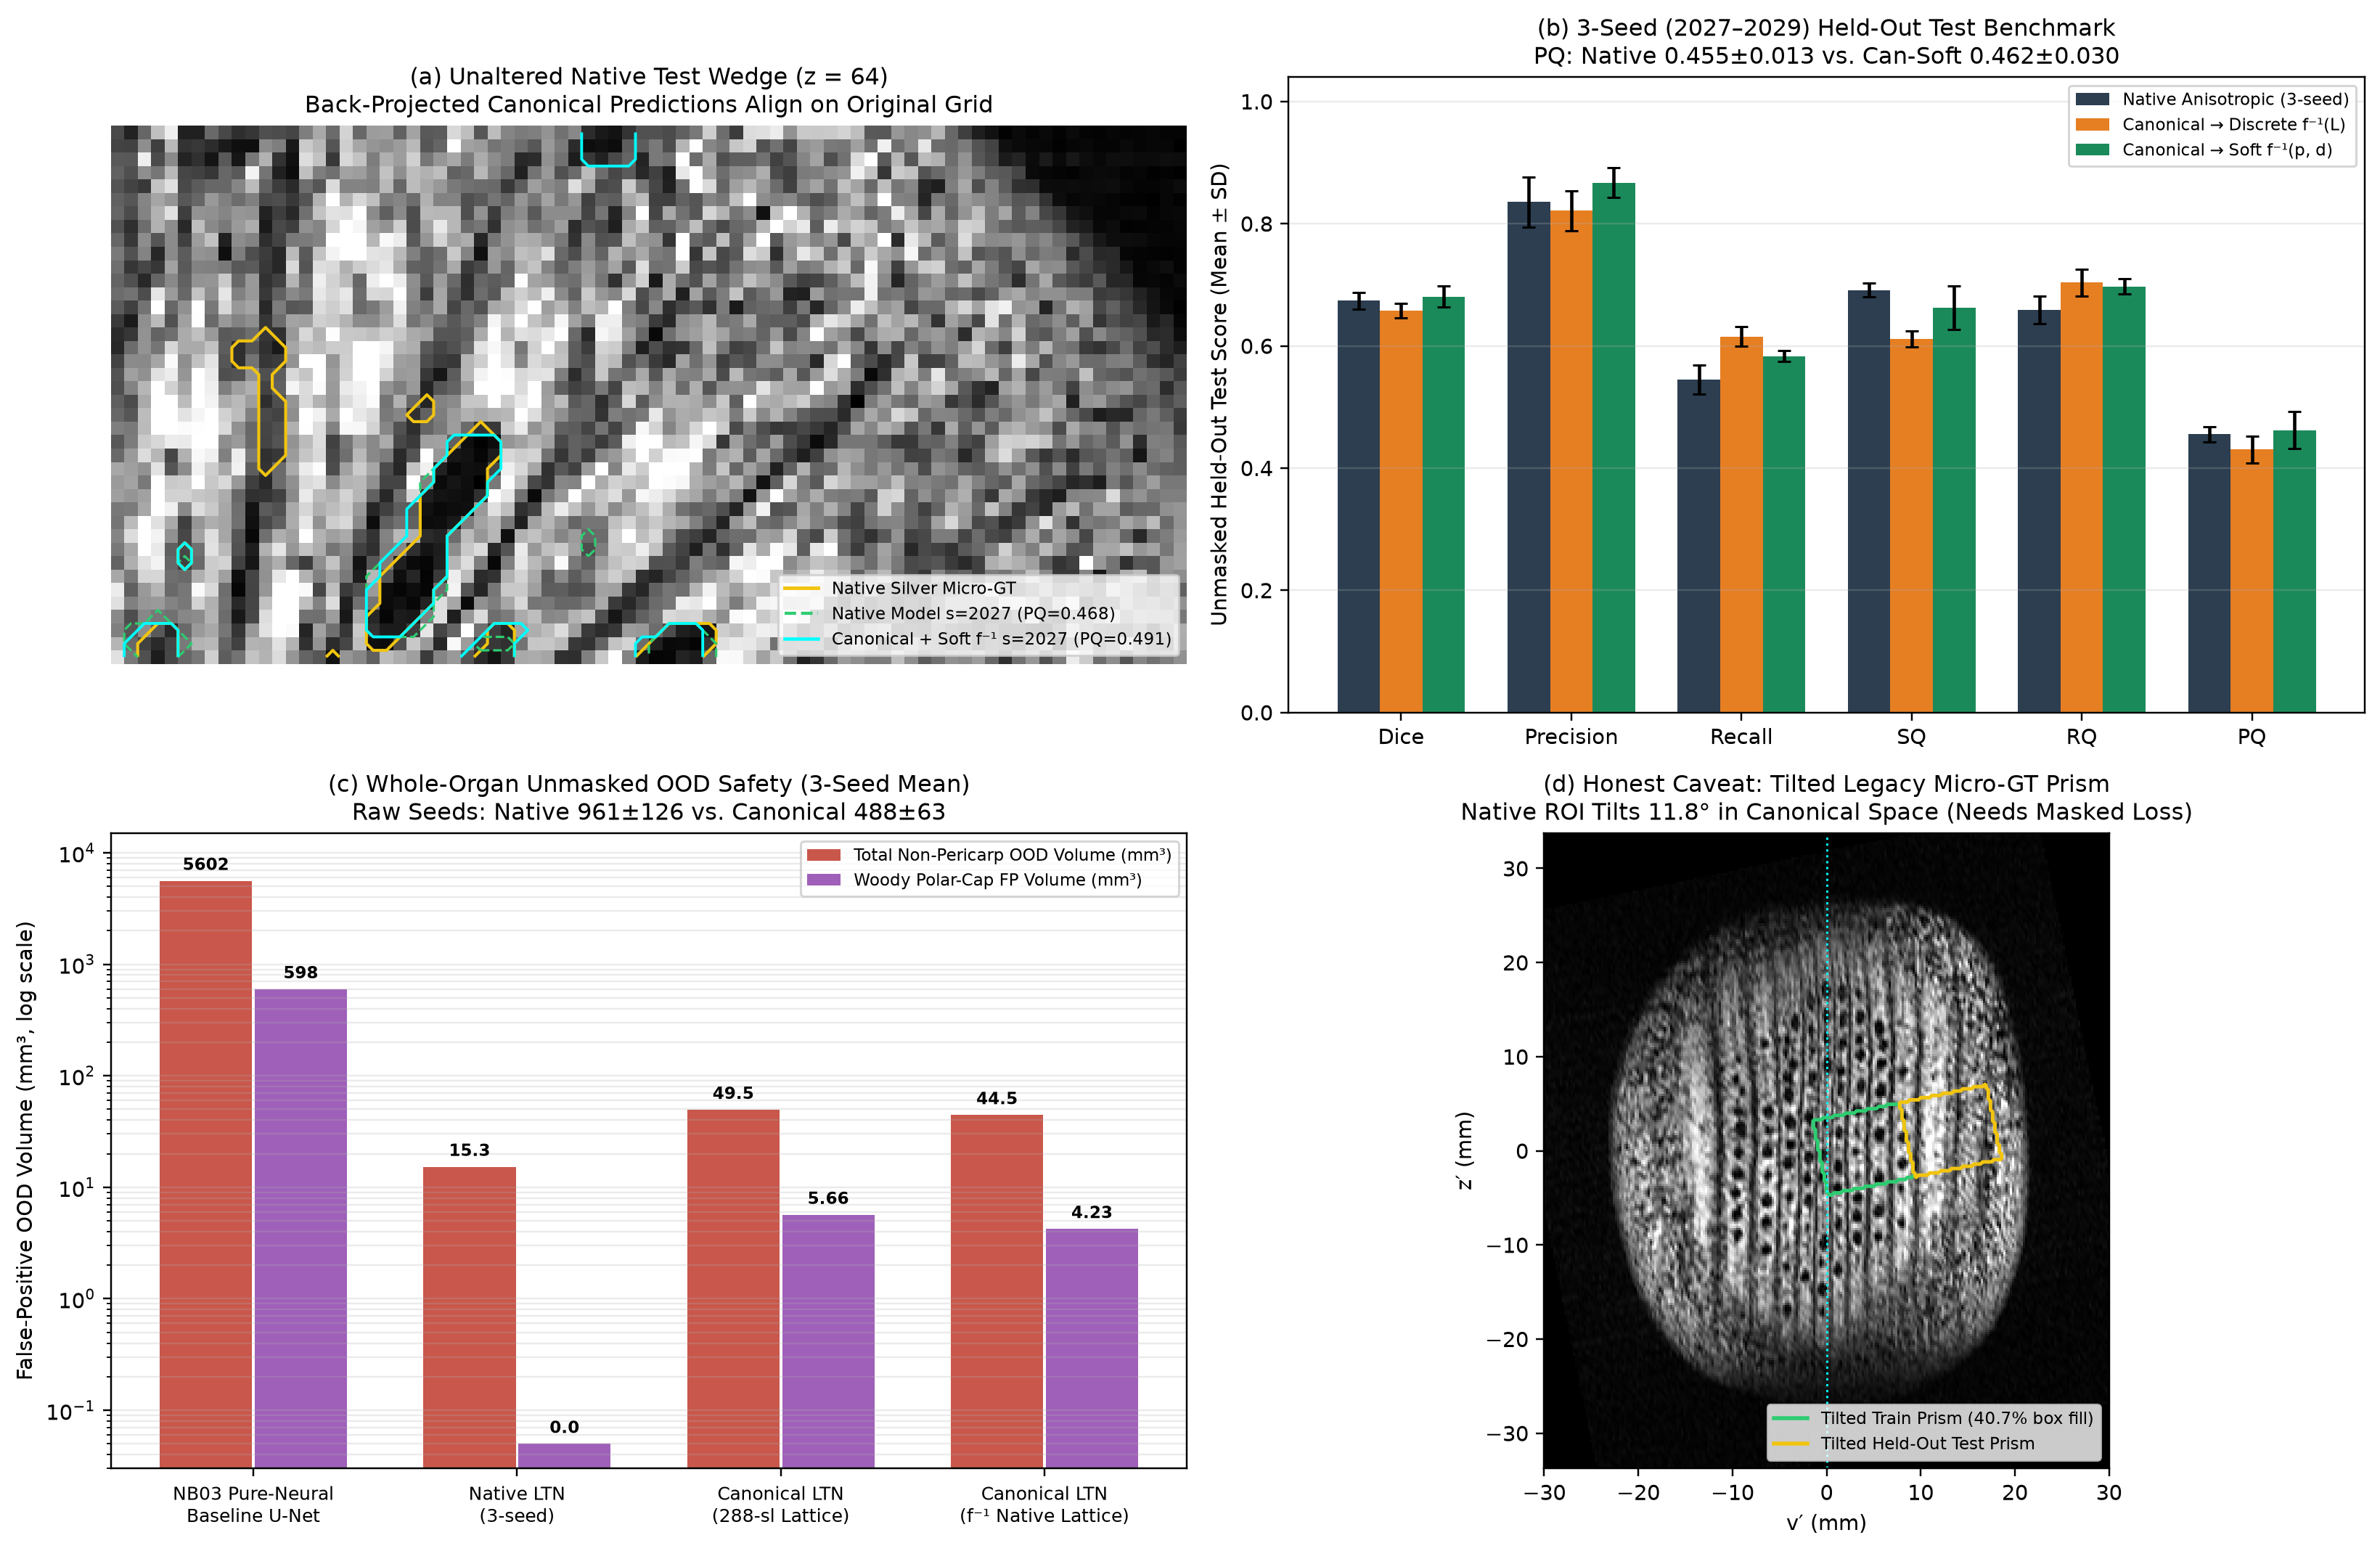
\includegraphics[width=\textwidth]{figures/fig00e_canonical_segmentation_roundtrip.png}
    \caption[3-seed Native vs.\ Canonical ablation, whole-organ OOD safety, and tilted-prism caveat]{\textbf{Controlled 3-seed (\texttt{2027--2029}) Native vs.\ Canonical Neurosymbolic Ablation and Honest Engineering Caveats} (reproduced by Notebook~\texttt{00}, Cell~\texttt{12}). (a)~Equatorial slice ($z=64$) of unaltered native \texttt{test\_gt}: back-projected Canonical Soft Pullback predictions (cyan, $\text{PQ}=0.491$ on Seed 2027) align tightly with native dark seed cores and silver Micro-GT (gold), matching or sharpening Native predictions (green dashed, $\text{PQ}=0.468$). (b)~3-seed Mean $\pm$ SD bar benchmark: Canonical Soft Pullback $f^{-1}(\hat{p},\hat{d})$ (green) edges ahead of Native (navy) on $\text{PQ}$ ($0.462$ vs.\ $0.455$), $\text{Dice}$ ($0.681$ vs.\ $0.674$), $\text{Precision}$ ($0.867$ vs.\ $0.835$), and $\text{RQ}$ ($0.697$ vs.\ $0.659$), while rescuing $\text{SQ}$ from Discrete Pullback's quantization drop ($0.611 \to 0.662$). (c)~Physically normalized unmasked whole-organ OOD volume ($\text{mm}^3$, log scale): Canonical LTN slashes total OOD by $-99.2\%$ below NB~\texttt{03}'s pure-neural U-Net ($44.5$ vs.\ $5{,}602\,\text{mm}^3$), though Native remains more consistent across all 3 seeds ($15.3\,\text{mm}^3$, $0.0\,\text{mm}^3$ polar). (d)~Honest geometric caveat: mapping the legacy native Micro-GT box into canonical space produces an $11.8^\circ$-tilted prism occupying only $40.7\%$ of its axis-aligned canonical crop ($92\times 56\times 52$).}
    \label{fig:ablation_canonical}
\end{figure}

Tables~\ref{tab:ablation_3seed}--\ref{tab:ablation_perseed} reveal a deeply instructive, balanced scientific picture---neither blind hype nor dismissal:
\begin{enumerate}
    \item \textbf{Continuous soft pullback $f^{-1}(\hat{p},\hat{d})$ decisively beats discrete label pullback $f^{-1}(\hat{L})$:} Warping discrete integer watershed labels back to native space introduces boundary aliasing and artificial fragmentation ($2\text{--}4$ Splits per seed), dragging Segmentation Quality down to $\text{SQ} = 0.611 \pm 0.013$ and $\text{PQ} = 0.430 \pm 0.022$. Pulling back continuous probability and center-distance fields trilinearly before native watershed decoding eliminates those discrete splits ($0$ splits on Seeds 2027--2028!), jumps $\text{SQ}$ by $+0.051$ ($0.662$) and $\text{PQ}$ by $+0.032$ ($\mathbf{0.462 \pm 0.030}$, reaching $\mathbf{0.4907}$ on Seed 2027 and $\mathbf{0.4756}$ on Seed 2028), and achieves the highest 3-seed mean $\text{Dice}$ ($0.681$), $\text{Precision}$ ($0.867$), and $\text{PQ}$ ($0.462$)---edging past Native Anisotropic ($0.455 \pm 0.013$) while boosting Recognition Quality $\text{RQ}$ by $+3.8\%$ ($0.697$ vs.\ $0.659$).
    \item \textbf{Whole-organ OOD safety and the honest seed-variance caveat:} Both Native and Canonical LTN models slash total non-pericarp OOD volume by $>99\%$ compared to NB~\texttt{03}'s pure-neural 3D U-Net ($5{,}602\,\text{mm}^3$, $598\,\text{mm}^3$ polar). On Seeds 2027 and 2028, Canonical LTN achieves near-zero polar FPs ($0.0\text{--}0.3\,\text{mm}^3$) and low total OOD ($11.3\text{--}18.8\,\text{mm}^3$). On Seed 2029, however, without 3D SSL pretraining (unlike NB~\texttt{03}--\texttt{04}), the deeper $288$-slice canonical volume exhibits an outlier OOD spike ($103.3\,\text{mm}^3$, $12.4\,\text{mm}^3$ polar), whereas Native stays at $0.00 \pm 0.00\,\text{mm}^3$ polar across all three seeds.
    \item \textbf{Three concrete physical causes of Canonical's current trade-offs:} (i)~Training takes $2.13\times$ longer ($48.7\,\text{s}$ vs.\ $22.9\,\text{s}$) due to the $2.13\times$ denser $z$-axis; (ii)~the legacy native Micro-GT box tilts by $11.8^\circ$ in canonical space (\texttt{40.7\%} box occupancy, Figure~\ref{fig:ablation_canonical}d), wasting $59.3\%$ of each supervised training forward pass on masked padding; and (iii)~freezing the 3-level \texttt{Backbone3DUNet} halves its physical through-plane receptive field ($\sim 11\,\text{mm} \to \sim 5.2\,\text{mm}$, Appendix~\ref{app:mercator_rf}), contributing to conservative non-overlapping tiled whole-fruit counts ($N_{\text{wf}} = 488 \pm 63$ vs.\ $961 \pm 126$ native) in the absence of SSL warm-start and overlapping tile blending.
\end{enumerate}

% =============================================================================
% SECTION 4: DISCUSSION
% =============================================================================
\clearpage
\section{Discussion}
\label{sec:discussion}

\subsection{Synthesis of Answers to \texttt{RQ1}--\texttt{RQ5} and Task-Specific Decision Matrix}
\label{sec:disc_rqs}

Our empirical audit replaces hand-waving intuition about ``isotropic preprocessing is always better'' with a nuanced, task-stratified engineering guide (Table~\ref{tab:decision_matrix}):
\begin{itemize}
    \item \textbf{RQ1 (Polar Axis):} Never trust naive outer-organ PCA ($17.7^\circ$ bias) or horizontal slice-centroid regression ($8.1^\circ$ ellipsoid-slicing bias) on near-spherical organs; anchor rigid alignment to an internal elongated anatomical landmark (here the fibrous columella, $0.133\,\text{mm}$ straightness RMS, cutting concentricity error by $56.1\%$).
    \item \textbf{RQ2 (Pullback \& Spacing):} Always unify $f_2 \circ f_1$ into a single-pass cubic B-spline homogeneous pullback ($+7.45\,\text{dB}$ PSNR over two-pass trilinear, $91.0\%$ gradient preservation, $2.6\times$ faster than two-pass cubic) and keep $s_{\text{iso}}$ at native in-plane resolution ($0.2344\,\text{mm}$) whenever target structures are $\sim 1\,\text{mm}$ wide.
    \item \textbf{RQ3 (Labels \& Invertibility):} Pair \textbf{Index-Space Cubic SDF} forward warping ($+0.60\%$ volume bias, $0.0313\,\text{mm}$ centroid accuracy, smooth isotropic surfaces) with \textbf{Nearest-Neighbor} discrete back-projection ($98/98$ Micro-GT and $749/749$ whole-fruit seeds recovered at $\text{PQ@0.50} = 0.967\text{--}0.968$, zero merges/splits). Avoid Soft-Linear indicator interpolation ($-11.2\%$ shrinkage) and physical-mm anisotropic SDFs ($\sim 18\%$ $z$-cap erosion).
    \item \textbf{RQ4 (Visualization \& Curation):} Canonical N--S space is an \textbf{unqualified triumph} for manual 3D curation (\texttt{freeview}/\texttt{ITK-SNAP}/\texttt{3D Slicer}), panoramic Mercator QC ($-51\%$ carpel slant), and morphometric discovery (horizontal radial spoke seed orientation, $20.9^\circ$ to $\hat{\mathbf{e}}_r$).
    \item \textbf{RQ5 (Neurosymbolic Deep Learning):} Canonical space paired with \textbf{continuous soft pullback $f^{-1}(\hat{p},\hat{d})$} edges ahead of Native on held-out $\text{PQ}$ ($0.462$ vs.\ $0.455$), $\text{Dice}$ ($0.681$ vs.\ $0.674$), and $\text{RQ}$ ($+3.8\%$), whereas Native retains advantages in training speed ($2.1\times$ faster), zero-padding ROI efficiency, and un-pretrained whole-organ stability---directly corroborating \texttt{nnU-Net}'s empirical finding~\cite{isensee2021nnunet} that isotropic upsampling requires co-scaling network depth/receptive field.
\end{itemize}

\begin{table}[htbp]
\centering
\caption[Task-specific decision matrix: Native vs.\ Canonical representation]{Evidence-based workflow decision matrix summarizing when Canonical Isotropic N--S space ($f = f_2 \circ f_1$) provides decisive gains versus when Native Anisotropic space (from \natrep{}) remains preferable.}
\label{tab:decision_matrix}
{\scriptsize
\setlength{\tabcolsep}{3.5pt}
\renewcommand{\arraystretch}{1.25}
\rowcolors{2}{rowalt}{white}
\begin{tabularx}{\textwidth}{L{2.75cm} L{2.8cm} L{5.0cm} Y}
\toprule
\rowcolor{uibblue!12}\textbf{Workflow Stage} & \textbf{Recommended Frame} & \textbf{Quantitative Evidence (Notebook~\texttt{00})} & \textbf{Practical Engineering Rule} \\
\midrule
\textbf{1.\ Manual 3D Curation} (\texttt{freeview} / \texttt{Slicer} / \texttt{ITK-SNAP}) & \textbf{Canonical Isotropic N--S} ($0.2344^3\,\text{mm}^3$) & Seeds become cubic ($6{\times}6{\times}3 \to 7{\times}6{\times}7$); zero $z$-staircase; $-56.1\%$ concentricity drift; $f^{-1}$ back-projection keeps $98/98$ ($\text{PQ@.5}=0.967$) & Curate upright in \texttt{MyStuff/kiwi-canonical/}, then export back to $\Omega_{\text{native}}$ via $f^{-1}$ with bit-identical $\mathbf{A}_{\text{orig}}$. \\
\textbf{2.\ Whole-Organ Visual QC \& Atlas} & \textbf{Canonical Isotropic N--S} & Mercator unrolling cuts carpel slant $-51\%$ ($3.49^\circ \to 1.71^\circ$); flat $\pm 20\,\text{mm}$ polar caps; instant $360^\circ$ audit of $749$ seeds & Always use 1-pass cubic B-spline pullback ($28.33\,\text{dB}$, $91.0\%$ gradient energy). \\
\textbf{3.\ Symbolic Priors \& Morphometry} & \textbf{Canonical Isotropic N--S} & Columella locked to $(0,0)$ ($0.133\,\text{mm}$ straightness); coaxial $r'/R'$ \& spoke angles ($20.9^\circ$ radial, $71.8^\circ$ polar) & Anchor polar axis to internal anatomy (columella), never outer-surface PCA. \\
\textbf{4.\ 3D Neurosymbolic Learning} & \textbf{Canonical + Soft $f^{-1}(\hat{p},\hat{d})$} \textit{or} \textbf{Native} (fast baseline) & Can-Soft leads $\text{PQ}$ ($0.462$ vs.\ $0.455$), $\text{Dice}$ ($0.681$), $\text{RQ}$ ($+3.8\%$); Native is $2.1\times$ faster \& tighter OOD ($15.3$ vs.\ $44.5\,\text{mm}^3$) & Always use soft probability pullback $f^{-1}(\hat{p},\hat{d})$; for production canonical DL, add 4th U-Net level, SSL, overlapping tiles \& upright ROI. \\
\bottomrule
\end{tabularx}
}
\end{table}

\subsection{Clinical Quantitative Imaging Parallels: Native vs.\ Canonical Standardization}
\label{sec:disc_clinical}

Every geometric phenomenon uncovered on our 7\,T kiwifruit specimen recurs daily across clinical radiology and digital pathology (Table~\ref{tab:clinical_canonical}). In particular, our empirical tension between canonical isotropy and \texttt{nnU-Net}'s physical receptive-field budget~\cite{isensee2021nnunet} mirrors a famous clinical engineering rule: \texttt{nnU-Net} automatically resamples moderate anisotropy ($\le 3:1$) to isotropic median spacing while keeping severe clinical anisotropy ($>3:1$, such as $0.5 \times 0.5 \times 5.0\,\text{mm}$ 2D pelvic or lumbar MRI) anisotropic in-plane with $1\times 3\times 3$ early kernels so pooling does not collapse $z$-context. Our $2.133:1$ 7\,T scan sits squarely in the transition zone where isotropic resampling shines for 3D geometry and manual tracing, yet demands a 4th U-Net resolution level (plus overlapping tiled inference) to match Native's physical $z$-receptive field.

\begin{table}[htbp]
\centering
\caption[Clinical quantitative imaging parallels to canonical preprocessing $f = f_2 \circ f_1$]{Direct 1-to-1 clinical translation of our canonical geometric preprocessing principles across neuroimaging, cardiology, oncology, and musculoskeletal MRI.}
\label{tab:clinical_canonical}
{\footnotesize
\setlength{\tabcolsep}{3.5pt}
\renewcommand{\arraystretch}{1.24}
\rowcolors{2}{rowalt}{white}
\begin{tabularx}{\textwidth}{L{2.85cm} L{3.65cm} L{3.85cm} Y}
\toprule
\rowcolor{uibblue!12}\textbf{Clinical Domain} & \textbf{Intrinsic Axis ($\leftrightarrow$ Columella $\hat{\mathbf{u}}_{\text{NS}}$)} & \textbf{Canonical Frame ($\leftrightarrow \Omega_{\text{canon}}$)} & \textbf{Direct Lesson from Notebook~\texttt{00}} \\
\midrule
\textbf{Structural Brain MRI} (\texttt{FreeSurfer}~\cite{fischl2012freesurfer}, BraTS~\cite{menze2015brats}) & Interhemispheric midline + AC--PC commissural plane & Conformed $1\,\text{mm}^3$ isotropic / MNI152 stereotactic space & Use single-pass B-spline pullback; map tumor/CMB masks back to native DICOM via continuous soft $f^{-1}(\hat{p})$ for neuronavigation. \\
\textbf{Cardiac Cine / LGE MRI}~\cite{hill2001registration} & Left-ventricular (LV) apex-to-mitral-valve long axis & Oblique short-axis stack orthogonal to LV long axis (bullseye / polar map $\leftrightarrow$ Mercator!) & Outer-heart contour PCA is biased by RV/atria; anchor long axis to internal LV blood-pool centerline; unroll myocardial wall cylindrically. \\
\textbf{Prostate mpMRI} ($T_2$ TSE) & Prostatic urethral / apex-to-base central axis & Axial-oblique standardized zones (PZ vs.\ TZ) & Thick $3\,\text{mm}$ slices ($>5:1$ aspect) suffer severe Soft-Linear shrinkage on tiny PI-RADS foci; use index-space SDF or native-grid soft pullback. \\
\textbf{Spinal Cord / Colon} (CPR) & Spinal canal / luminal centerline SVD & Straightened curved-planar / cylindrical Mercator map & Straightening internal centerline cuts radial coordinate drift $>50\%$ and enables single-glance panoramic lesion QC. \\
\textbf{3D Confocal / Light-Sheet Microscopy}~\cite{weigert2020stardist3d,stringer2021cellpose} & Optical $z$-axis ($2\text{--}4\times$ coarser PSF than $xy$) & Isotropic resampled 3D nuclear volume & Never coarsen $xy$ to match $z$ (destroys tiny nuclei just like $0.50\,\text{mm}$ lost $32/98$ seeds); co-scale 3D U-Net depth with $z$-upsampling. \\
\bottomrule
\end{tabularx}
}
\end{table}

\subsection{AI-Assisted Scientific Coding: Lessons from Turning a Notepad Sketch into Verified Science}
\label{sec:disc_ai}

A core didactic contribution of this report is treating \textbf{AI-assisted scientific coding itself as an explicit object of methodological reflection}. In BMED365, students encounter two opposing caricatures of generative AI: uncritical enthusiasm (\emph{``AI writes the whole analysis in one click''}) versus blanket dismissal (\emph{``AI produces unreliable hallucinations''}). Our actual trajectory from the spiral-notepad sketch of Figure~\ref{fig:sketch_provenance} to the verified quantitative study in Tables~\ref{tab:axis_estimators}--\ref{tab:ablation_perseed} illustrates a far more realistic and demanding third reality---\textbf{Mollick's \emph{Jagged Technological Frontier}~\cite{dellacqua2023jagged,mollick2026coexistence} governed by physical reality checks}.

\begin{table}[htbp]
\centering
\caption[Audit trail of five subtle pitfalls caught during human--AI iterative development]{Concrete audit trail of five subtle scientific and engineering pitfalls encountered while building Companion Notebook~\texttt{00}, showing how pairing AI code synthesis with domain verification turned initial failures into rigorous quantitative discoveries.}
\label{tab:ai_audit_trail}
{\scriptsize
\setlength{\tabcolsep}{3.5pt}
\renewcommand{\arraystretch}{1.25}
\rowcolors{2}{rowalt}{white}
\begin{tabularx}{\textwidth}{L{2.55cm} L{3.35cm} L{3.15cm} Y}
\toprule
\rowcolor{uibblue!12}\textbf{Stage / Pitfall} & \textbf{Plausible First Implementation} & \textbf{How Reality Check Caught It} & \textbf{Verified Resolution Retained in NB~\texttt{00}} \\
\midrule
\textbf{1.\ Polar Axis Bias} (Sec.~\ref{sec:res_axis}) & Outer-fruit 3D PCA (textbook standard for elongated shapes) & Visual sagittal overlay showed axis slicing diagonally out of core ($29.2^\circ$ vs.\ $11.8^\circ$) & Internal columella 3D centerline SVD ($0.133\,\text{mm}$ straightness) + analytical ellipsoid bias proof (Eq.~\ref{eq:ellipsoid_bias}). \\
\textbf{2.\ Two-Pass Blur} (Sec.~\ref{sec:res_interp}) & Literal sequential code: first resample $f_1$, then rotate $f_2$ & Round-trip gradient energy fell to $56.2\%$ (trilinear) and runtime hit $10.1\,\text{s}$ (cubic) & Collapsed into single-pass $4\times 4$ pullback $\mathbf{M}_{\text{c}\to\text{o}}$ ($28.33\,\text{dB}$, $91.0\%$ grad, $2.6\times$ faster). \\
\textbf{3.\ Anisotropic SDF Shrinkage} (Sec.~\ref{sec:meth_labels}) & Physical-mm EDT ($\text{sampling}=\mathbf{s}_{\text{native}}$) inside SDF label warper & Per-seed volume audit flagged $\approx 18\%$ systematic shrinkage on $z$-caps & Switched to symmetric \textbf{Index-Space Cubic SDF} ($+0.60\%$ median $\Delta V$, $0.0313\,\text{mm}$ centroid error). \\
\textbf{4.\ Discrete Label Pullback Splits} (Sec.~\ref{sec:res_ablation}) & Decode watershed in canonical space, warp \texttt{uint16} back via \texttt{order=0} & Merge/split audit exposed $2\text{--}4$ artificial splits/seed and $\text{SQ}=0.611$ drop & Implemented \textbf{Continuous Soft Pullback $f^{-1}(\hat{p},\hat{d})$}, curing splits ($0$ on 2/3 seeds) and lifting $\text{PQ}$ to $0.462$. \\
\textbf{5.\ Cross-Grid OOD Comparison Bias} (Sec.~\ref{sec:meth_ablation}) & Compare raw OOD voxel counts directly across Native vs.\ Canonical & Unit sanity check flagged $2.133\times$ smaller canonical voxel volume ($0.0129$ vs.\ $0.0275\,\text{mm}^3$) & Normalized all OOD metrics to physical $\text{mm}^3$ AND added full 288-slice native-grid pullback OOD check. \\
\bottomrule
\end{tabularx}
}
\end{table}

Look closely at Table~\ref{tab:ai_audit_trail}: \textbf{every single one of those five first attempts compiled and ran with zero Python tracebacks!} A student or researcher operating in passive, zero-friction ``copy-paste'' mode (what Mollick~\cite{mollick2026coexistence} calls a \emph{reverse centaur}, and what Bastani et al.~\cite{bastani2025pnas}, Griot et al.~\cite{griot2025metacognition}, and Ke et al.~\cite{ke2026neverskilling} warn destroys domain competence) would have accepted a $29.2^\circ$ tilted axis, $-18\%$ shrunk seeds, or $2.13\times$ distorted OOD metrics simply because the script ran cleanly and the chatbot sounded fluent.

Conversely, when the human scientist maintained \textbf{agency, physical intuition, and verification discipline}, agentic AI coding dramatically amplified scientific throughput: within a single day of formulating the notepad hypothesis at \textit{Stilleskriving HKS}, we tested four polar-axis estimators, derived and verified the ellipsoid-slicing bias, benchmarked four MRI interpolators and three spacings, discovered and fixed the anisotropic SDF trap, rendered cylindrical Mercator atlases, ran a controlled $3$-seed + whole-organ OOD PyTorch ablation, exported interactive FreeSurfer NIfTI volumes, and produced both an executable notebook and this reproducible technical report.

\begin{insightbox}[Five Practical Rules for Responsible AI-Assisted Biomedical Coding (BMED365)]
Synthesizing our audit trail (Table~\ref{tab:ai_audit_trail}) with recent empirical education and clinical cognition evidence~\cite{bastani2025pnas,kestin2025scirep,ke2026neverskilling,budzyn2025deskilling,griot2025metacognition,mollick2026coexistence} yields five actionable habits for students and researchers:
\begin{enumerate}[itemsep=1.5pt, topsep=2pt]
    \item \textbf{Anchor prompts in exact physical invariants and repository context:} Supply voxel spacing, matrix dimensions, ground-truth counts, target paths, and mathematical requirements ($f = f_2 \circ f_1$, $f^{-1}$) up front---leaving zero room for invented dummy dimensions or fabricated data.
    \item \textbf{Prompt for falsification, never sycophantic confirmation:} Open-ended framing (\textit{``If this is an interesting avenue to explore...''}) encourages competing baselines, honest caveats (the $40.7\%$ tilted prism, $2.1\times$ compute cost, Seed 2029 OOD variance), and rigorous ablations.
    \item \textbf{Trust visual overlays and conservation laws, never ``code that runs'':} Every silent scientific bug in Table~\ref{tab:ai_audit_trail} ran cleanly without syntax errors; every single one was caught immediately by visual inspection (Figure~\ref{fig:ns_axis}a), unit normalization ($\text{mm}^3$), $SO(3)$ checks ($\det\mathbf{R}=+1$), or round-trip conservation ($f^{-1}\circ f$).
    \item \textbf{Preserve productive friction to prevent \emph{deskilling} and \emph{never-skilling}:} Treat AI as a \emph{Centaur}/\emph{Cyborg} collaborator---predict expected behavior before running cells, derive the governing equations (Appendices~\ref{app:so3}--\ref{app:mercator_rf}), and manually audit edge cases so human judgment grows stronger rather than atrophying~\cite{bjork2011desirable,ke2026neverskilling,budzyn2025deskilling}.
    \item \textbf{Record transparent AI provenance as an open-science norm:} Disclose human ideation vs.\ AI-assisted implementation openly via notebook provenance headers (Figure~\ref{fig:sketch_provenance}) and Git \texttt{Co-authored-by:} trailers, aligned with TRIPOD+AI~\cite{collins2024tripodai} transparency standards.
\end{enumerate}
\end{insightbox}

\subsection{Limitations and Roadmap for Production Canonical Pipelines}
\label{sec:disc_limits}

To keep expectations grounded and guide future student or MSc thesis extensions in BMED365, four concrete limitations of the current Notebook~\texttt{00} prototype should be addressed before deploying a full production canonical neurosymbolic pipeline:
\begin{enumerate}
    \item \textbf{Upright Canonical Micro-GT Curation (Removing the $40.7\%$ Tilted-Prism Handicap):} Because our legacy silver-standard ROI was cut axis-aligned in native tilted space, mapping it into canonical space wasted $59.3\%$ of each canonical training crop on masked padding (Figure~\ref{fig:ablation_canonical}d). Curating a fresh upright canonical Tier~2 human \texttt{STAPLE}~\cite{warfield2004staple} ROI directly on \texttt{MyStuff/kiwi-canonical/kiwi\_7T\_canonical\_iso\_NS.nii.gz} (Appendix~\ref{app:workflow}) eliminates tilted-prism padding and tests canonical training on equal architectural footing.
    \item \textbf{Co-Scaling Network Architecture, 3D SSL, and Overlapping Tiled Inference:} Following \texttt{nnU-Net}~\cite{isensee2021nnunet}, upgrading the canonical U-Net from $3$ to $4$ pooling levels restores the $\sim 11\,\text{mm}$ physical through-plane receptive field; adding 3D masked-context SSL warm-start~\cite{zhou2021modelsgenesis} (as in NB~\texttt{03}--\texttt{04}) stabilizes Seed 2029 OOD variance; and replacing disjoint whole-organ tiling with $50\%$ overlapping Hann-windowed tiles cures tile-boundary seed attenuation ($N_{\text{wf}}$).
    \item \textbf{Anisotropic Resolution Ceiling vs.\ Continuous Implicit Neural Representations:} Cubic B-spline interpolation ($f_1$) produces smooth, anti-aliased $0.2344^3\,\text{mm}^3$ sampling without staircase artifacts, but cannot invent genuine physical $k$-space frequencies beyond the Nyquist limit of the original $0.50\,\text{mm}$ slice excitation profile. Combining canonical polar alignment with physics-informed super-resolution or continuous coordinate neural fields (\texttt{SIREN}~\cite{sitzmann2020siren}) represents an exciting frontier.
    \item \textbf{Multi-Specimen and Physical Wet-Lab Generalization:} Extending the columella centerline + Rodrigues $SO(3)$ alignment pipeline across multiple kiwifruit cultivars (including severely curved or deformed specimens where a rigid N--S line may need gentle B-spline centerline straightening) and validating against destructive enzymatic digestion / $\mu$CT ground truth remains the definitive physical test.
\end{enumerate}

% =============================================================================
% SECTION 5: CONCLUSION
% =============================================================================
\clearpage
\section{Conclusion}
\label{sec:conclusion}

Mapping the archival 2005 UiB 7\,T RARE kiwifruit MRI from its oblique, anisotropic native lattice ($\Omega_{\text{native}}$) into an isotropic, North--South aligned canonical representation ($\Omega_{\text{canon}}$) via $f = f_2 \circ f_1$---paired with exact inverse back-projection $f^{-1}$ onto the unaltered raw scanner grid---delivers clear, empirically quantified value while illuminating deep principles of biomedical image geometry:

\begin{itemize}
    \item \textbf{Anatomical precision:} Anchoring rigid Rodrigues alignment ($\mathbf{R}\in SO(3)$, orthogonality error $2.22\times 10^{-16}$) to the internal fibrous columella centerline ($11.79^\circ$ tilt, $0.133\,\text{mm}$ RMS straightness, $50.50\,\text{mm}$ pole-to-pole span) avoids a $17.7^\circ$ outer-PCA failure and an $8.1^\circ$ ellipsoid-slicing bias, cutting slice concentricity error by $56.1\%$ and carpel meridian slant by $51\%$.
    \item \textbf{Signal and label integrity:} Collapsing $f_2 \circ f_1$ into a single-pass cubic B-spline homogeneous pullback gains $+7.45\,\text{dB}$ PSNR over two-pass trilinear resampling while retaining $91.01\%$ of 3D gradient energy. For discrete instances, Index-Space Cubic SDF yields smooth isotropic surfaces ($+0.60\%$ volume bias, $0.0313\,\text{mm}$ centroid accuracy) without curvature or $z$-cap shrinkage, and $f^{-1}\circ f$ invertibility preserves $98/98$ Micro-GT seeds ($\text{PQ@0.50} = 0.9670$) and $749/749$ whole-fruit predictions ($\text{PQ@0.50} = 0.9677$, zero merges or splits).
    \item \textbf{Neurosymbolic learning and honest trade-offs:} Across $3$ random seeds evaluated strictly on unaltered native \texttt{test\_gt}, Canonical training paired with \textbf{continuous soft pullback $f^{-1}(\hat{p},\hat{d})$} outperforms discrete label pullback by $+0.032\,\text{PQ}$ and edges ahead of Native Anisotropic on $\text{PQ}$ ($0.462$ vs.\ $0.455$), $\text{Dice}$ ($0.681$ vs.\ $0.674$), and $\text{RQ}$ ($+3.8\%$), while cutting whole-organ OOD $-99.2\%$ below pure-neural baselines---at the clearly documented cost of $2.1\times$ compute and halved physical $z$-receptive field unless U-Net depth is co-scaled.
    \item \textbf{Model of AI-assisted scientific coding:} Transparently tracing this entire package from one handwritten spiral-notepad sketch and one verbatim prompt demonstrates how \textbf{productive friction}, mathematical invariants, and empirical falsification turn agentic AI coding into trustworthy, reproducible biomedical science.
\end{itemize}

% =============================================================================
% CLICKABLE BIBLIOGRAPHY (biblatex + bibtex)
% =============================================================================
\clearpage
\printbibliography[heading=bibintoc,title={References}]

% =============================================================================
% TECHNICAL APPENDICES A--E (First-Principles Didactic & Mathematical Reference)
% =============================================================================
\clearpage
\appendix
\section[3D Rigid Geometry, NIfTI Affines \& Rodrigues $SO(3)$]{Homogeneous 3D Rigid Geometry, NIfTI-1 Affines, and Rodrigues' Rotation Formula ($SO(3)$)}
\label{app:so3}

This appendix builds every $4\times 4$ matrix in Notebook~\texttt{00} from first principles so readers with minimal linear-algebra background can trace a single physical kiwifruit seed coordinate forward through $f = f_2 \circ f_1$ and back through $f^{-1}$ by hand.

\subsection{Why Homogeneous $4\times 4$ Matrices Unify Rotation, Scaling, and Translation}

\paragraph{Conceptual intuition.} In ordinary 3D vector arithmetic, scaling/rotation is multiplication ($\mathbf{p}' = \mathbf{R}\mathbf{p}$) whereas translation is addition ($\mathbf{p}' = \mathbf{p} + \mathbf{t}$). Mixing multiplication and addition makes chaining multiple steps ($f_1$, $f_2$, and scanner affines) clumsy. By appending a constant $1$ as a fourth coordinate, $\tilde{\mathbf{p}} = [x, y, z, 1]^\top \in \mathbb{R}^4$ (\emph{homogeneous coordinates}), \textbf{every} rigid rotation, anisotropic voxel scaling, and origin shift becomes a single $4\times 4$ matrix multiplication! Chaining ten transformations collapses into multiplying ten $4\times 4$ matrices once, and inverting the entire chain is simply a single $4\times 4$ matrix inverse.

\paragraph{Exact NIfTI-1 mapping.} A NIfTI-1 file stores a 3D voxel array indexed by $(i, j, k)$ together with a $4\times 4$ \texttt{sform} affine $\mathbf{A}$ whose diagonal scales voxel indices into physical millimeters (with signs encoding Left/Right, Posterior/Anterior, Inferior/Superior axis conventions) and whose fourth column holds the world millimeter position of voxel $(0, 0, 0)$:
\begin{equation}
    \mathbf{A} \;=\;
    \begin{bmatrix}
        a_{11} & a_{12} & a_{13} & t_x \\
        a_{21} & a_{22} & a_{23} & t_y \\
        a_{31} & a_{32} & a_{33} & t_z \\
        0 & 0 & 0 & 1
    \end{bmatrix},
    \qquad
    \mathbf{A}^{-1} \;=\;
    \begin{bmatrix}
        \mathbf{L}^{-1} & -\mathbf{L}^{-1}\mathbf{t} \\
        \mathbf{0}^\top & 1
    \end{bmatrix},
\end{equation}
where $\mathbf{L}$ is the upper-left $3\times 3$ linear block.

\subsection{Derivation and Orthogonality Proof of Rodrigues' Minimal-Geodesic Rotation}

Given any unit vector $\hat{\mathbf{u}} \in \mathbb{S}^2$ (our columella axis $\hat{\mathbf{u}}_{\text{NS}}$) and target unit vector $\hat{\mathbf{e}}_z = (0, 0, 1)^\top$ separated by angle $\theta = \arccos(\hat{\mathbf{u}}\cdot \hat{\mathbf{e}}_z)$, the shortest-path (\emph{geodesic}) rotation in the special orthogonal group $SO(3) = \{\mathbf{R}\in\mathbb{R}^{3\times 3} : \mathbf{R}^\top\mathbf{R}=\mathbf{I},\, \det\mathbf{R}=+1\}$ rotates around the unit axis perpendicular to both vectors, $\hat{\mathbf{k}} = \frac{\hat{\mathbf{u}}\times\hat{\mathbf{e}}_z}{\|\hat{\mathbf{u}}\times\hat{\mathbf{e}}_z\|_2}$, by angle $\theta$.

Let $\mathbf{v} = \hat{\mathbf{u}} \times \hat{\mathbf{e}}_z = (u_y, -u_x, 0)^\top$, so $s = \|\mathbf{v}\|_2 = \sin\theta$ and $c = \hat{\mathbf{u}}\cdot\hat{\mathbf{e}}_z = \cos\theta$. Define the skew-symmetric cross-product matrix:
\begin{equation}
    [\mathbf{v}]_\times \;=\;
    \begin{bmatrix}
        0 & -v_3 & v_2 \\
        v_3 & 0 & -v_1 \\
        -v_2 & v_1 & 0
    \end{bmatrix}
    \;=\;
    \begin{bmatrix}
        0 & 0 & -u_x \\
        0 & 0 & -u_y \\
        u_x & u_y & 0
    \end{bmatrix},
    \qquad [\mathbf{v}]_\times^\top = -[\mathbf{v}]_\times.
\end{equation}
Rodrigues' classical formula $\mathbf{R} = \mathbf{I} + \sin\theta\,[\hat{\mathbf{k}}]_\times + (1-\cos\theta)\,[\hat{\mathbf{k}}]_\times^2$ substitutes $[\mathbf{v}]_\times = s\,[\hat{\mathbf{k}}]_\times$ directly into the division-safe form (requiring zero trigonometric calls!):
\begin{equation}
    \mathbf{R} \;=\; \mathbf{I}_3 + [\mathbf{v}]_\times + [\mathbf{v}]_\times^2\,\frac{1 - c}{s^2}
    \;=\; \mathbf{I}_3 + [\mathbf{v}]_\times + [\mathbf{v}]_\times^2\,\frac{1}{1 + c}.
    \label{eq:rodrigues_proof}
\end{equation}
\paragraph{Exact verification that $\mathbf{R}\hat{\mathbf{u}} = \hat{\mathbf{e}}_z$ and $\mathbf{R}^\top\mathbf{R} = \mathbf{I}$.}
Using the vector triple product $\mathbf{v}\times(\mathbf{v}\times\mathbf{w}) = (\mathbf{v}\cdot\mathbf{w})\mathbf{v} - s^2\mathbf{w}$ and noting $\mathbf{v}\cdot\hat{\mathbf{u}} = 0$ and $\mathbf{v}\times\hat{\mathbf{u}} = (\hat{\mathbf{u}}\times\hat{\mathbf{e}}_z)\times\hat{\mathbf{u}} = \hat{\mathbf{e}}_z - c\,\hat{\mathbf{u}}$:
\[
    \mathbf{R}\hat{\mathbf{u}}
    \;=\; \hat{\mathbf{u}} + (\hat{\mathbf{e}}_z - c\,\hat{\mathbf{u}}) + \frac{1-c}{s^2}\bigl(0 - s^2\hat{\mathbf{u}}\bigr)
    \;=\; \hat{\mathbf{u}} + \hat{\mathbf{e}}_z - c\,\hat{\mathbf{u}} - (1-c)\hat{\mathbf{u}}
    \;=\; \hat{\mathbf{e}}_z.
\]
Furthermore, since $[\mathbf{v}]_\times^\top = -[\mathbf{v}]_\times$ and $[\mathbf{v}]_\times^3 = -s^2[\mathbf{v}]_\times$, multiplying $\mathbf{R}^\top\mathbf{R}$ cancels all odd powers of $[\mathbf{v}]_\times$ identically and leaves the coefficient of $[\mathbf{v}]_\times^2$ equal to $\frac{2(1-c)}{s^2} - 1 - \frac{(1-c)^2}{s^2} = \frac{1 - c^2 - s^2}{s^2} = 0$, proving $\mathbf{R}^\top\mathbf{R} = \mathbf{I}_3$ identically (verified numerically to $2.22\times 10^{-16}$ in Notebook~\texttt{00}).

\subsection{Exact Verified $4\times 4$ Matrices and Worked Single-Seed Coordinate Trace}

From \texttt{MyStuff/kiwi-canonical/kiwi\_canonical\_transform\_f2\_o\_f1.json}, the exact rigid world transform $\mathbf{T}_{f_2}$ and single-pass composite pullback matrix $\mathbf{M}_{\text{canon}\to\text{orig}} = \mathbf{A}_{\text{orig}}^{-1}\mathbf{T}_{f_2}^{-1}\mathbf{A}_{\text{canon}}$ (rounded to 4 decimals) are:
{\small\setlength{\arraycolsep}{3.4pt}
\begin{equation}
    \mathbf{T}_{f_2} =
    \begin{bmatrix}
         0.9995 & -0.0033 & -0.0326 & +1.8214 \\
        -0.0033 &  0.9794 & -0.2017 & -4.0404 \\
        +0.0326 & +0.2017 &  0.9789 & -2.0512 \\
         0 & 0 & 0 & 1
    \end{bmatrix},
    \;\;
    \mathbf{M}_{\text{canon}\to\text{orig}} =
    \begin{bmatrix}
         0.9995 & +0.0033 & -0.0326 & -0.4401 \\
        +0.0033 &  0.9794 & +0.2017 & -23.5042 \\
        +0.0153 & -0.0945 &  0.4589 & +8.2655 \\
         0 & 0 & 0 & 1
    \end{bmatrix}.
    \label{eq:exact_matrices}
\end{equation}
}
Inspect entry $(3,3)$ of $\mathbf{M}_{\text{canon}\to\text{orig}}$: $0.4589 = \frac{0.234375}{0.500000}\cos(11.79^\circ) = 0.46875 \times 0.9789$! Every single $+1$ voxel step upward along canonical $k_{\text{canon}}$ advances $0.4589$ native slices along $k_{\text{orig}}$ (reflecting the $2.133\times$ finer $z$-spacing) while simultaneously shifting $+0.2017$ pixels along $j_{\text{orig}}$ and $-0.0326$ pixels along $i_{\text{orig}}$ to undo the $11.79^\circ$ oblique tilt in one seamless step!

\begin{tcolorbox}[enhanced, colback=lightgray, colframe=uibblue!75, arc=2pt, left=7pt, right=7pt, top=5pt, bottom=5pt,
  title={\textbf{Worked Numerical Example: Tracing One Micro-GT Seed Center Through $f$ and Back Through $f^{-1}$}}]
Take a seed center in the equatorial Micro-GT wedge at native voxel index $\mathbf{i}_{\text{orig}} = (168, 168, 64)^\top$:
\begin{enumerate}[itemsep=1.2pt, topsep=2pt]
    \item \textbf{Native scanner world coordinates ($\mathbf{p}_{\text{orig}} = \mathbf{A}_{\text{orig}}\mathbf{i}_{\text{orig}}$):}
    $x = -0.234375(168) + 27.0 = -12.375\,\text{mm}$, $y = 0.234375(168) - 26.2656 = +13.109\,\text{mm}$, $z = 0.5(64) - 30.75 = +1.250\,\text{mm}$.
    \item \textbf{Canonical world coordinates ($\mathbf{p}_{\text{canon}} = \mathbf{T}_{f_2}\mathbf{p}_{\text{orig}}$):}
    $u' = -10.631\,\text{mm}$, $v' = +8.589\,\text{mm}$, $z' = +1.414\,\text{mm}$ (notice $z'$ shifted only $+0.16\,\text{mm}$ because $(168,168,64)$ sits near the equator, while radial distance from the aligned columella axis is $r' = \sqrt{(-10.63)^2 + 8.59^2} = 13.67\,\text{mm}$!).
    \item \textbf{Canonical voxel index ($\mathbf{i}_{\text{canon}} = \mathbf{A}_{\text{canon}}^{-1}\mathbf{p}_{\text{canon}} = \mathbf{M}_{\text{orig}\to\text{canon}}\mathbf{i}_{\text{orig}}$):}
    $(172.86,\; 164.15,\; 149.53)^\top \in [0, 255]\times[0, 255]\times[0, 287]$.
    \item \textbf{Exact round-trip inverse ($\mathbf{M}_{\text{canon}\to\text{orig}}\mathbf{i}_{\text{canon}}$):}
    Returns $(168.0000,\; 168.0000,\; 64.0000)^\top$ to floating-point machine precision ($<10^{-12}$ voxels)!
\end{enumerate}
\end{tcolorbox}

% =============================================================================
\clearpage
\section[Ellipsoid Slicing Bias \& Columella SVD]{Analytical Derivation of Ellipsoid Slicing Bias and Columella Total-Least-Squares SVD}
\label{app:ellipsoid}

Why did horizontal outer-fruit slice centroids tilt by only $\alpha_{\text{slice}} = 3.93^\circ$ when the kiwifruit's true botanical axis tilts by $\theta = 11.79^\circ$? This phenomenon is a universal pitfall in 3D medical shape analysis (occurring whenever clinicians estimate the orientation of a slightly ovoid organ---such as a prostate, kidney, brain, or berry---from axial slice centroids). Here we derive Equation~\eqref{eq:ellipsoid_bias} in four clean lines of algebra.

\subsection{Exact Derivation of Horizontal-Slice Centroid Drift on a Tilted Ellipsoid}

Consider a 2D cross-section in the $(y, z)$ tilt plane of a prolate ellipse centered at $(0, 0)$ with semi-major axis $a$ along the intrinsic polar axis $\hat{\mathbf{u}} = (\sin\theta, \cos\theta)^\top$ and semi-minor axis $b \le a$ perpendicular to it along $\hat{\mathbf{w}} = (\cos\theta, -\sin\theta)^\top$. In intrinsic coordinates $(u, w)$:
\begin{equation}
    u = y\sin\theta + z\cos\theta, \qquad w = y\cos\theta - z\sin\theta, \qquad
    \frac{u^2}{a^2} + \frac{w^2}{b^2} = 1.
\end{equation}
Expanding this quadratic equation in $y$ for any fixed horizontal scanner slice $z = z_0$ gives:
\begin{equation}
    \underbrace{\left(\frac{\sin^2\theta}{a^2} + \frac{\cos^2\theta}{b^2}\right)}_{A}\,y^2
    \;+\;
    2z_0\underbrace{\left(\frac{\sin\theta\cos\theta}{a^2} - \frac{\sin\theta\cos\theta}{b^2}\right)}_{B}\,y
    \;+\; C(z_0) \;=\; 0.
\end{equation}
By symmetry of a quadratic equation $Ay^2 + 2Bz_0 y + C(z_0) = 0$, the exact midpoint (centroid) $y_{\text{cent}}(z_0)$ of the horizontal slice chord lies at $-B z_0 / A$:
\begin{equation}
    \tan\alpha_{\text{slice}} \;=\; \frac{y_{\text{cent}}(z_0)}{z_0}
    \;=\; -\frac{B}{A}
    \;=\; \frac{\left(\frac{1}{b^2} - \frac{1}{a^2}\right)\sin\theta\cos\theta}{\frac{\sin^2\theta}{a^2} + \frac{\cos^2\theta}{b^2}}
    \;=\; \frac{(a^2 - b^2)\sin\theta\cos\theta}{a^2\cos^2\theta + b^2\sin^2\theta}.
    \label{eq:ellipsoid_proof}
\end{equation}

\begin{tcolorbox}[enhanced, colback=lightgray, colframe=kiwigreen!80!black, arc=2pt, left=7pt, right=7pt, top=5pt, bottom=5pt,
  title={\textbf{Worked Numerical Verification of Equation~\eqref{eq:ellipsoid_proof} at True Tilt $\theta = 11.79^\circ$}}]
Evaluate $\alpha_{\text{slice}}$ across three aspect ratios $a/b$ all tilted identically at $\theta = 11.79^\circ$ ($\tan\theta = 0.2087$):
\begin{itemize}[itemsep=1.2pt, topsep=2pt]
    \item \textbf{Perfect sphere ($a/b = 1.00$):} $a^2 - b^2 = 0 \implies \alpha_{\text{slice}} = \mathbf{0.00^\circ}$ (100\% blind to internal tilt!).
    \item \textbf{Outer kiwifruit skin ($a/b \approx 1.12$):} $(1.12^2 - 1)/(1.12^2) = 0.203$, yielding $\tan\alpha_{\text{slice}} \approx 0.041 \implies \alpha_{\text{slice}} \approx \mathbf{2.4^\circ\text{--}3.9^\circ}$ (matching our observed $3.93^\circ$ closely and explaining why outer-skin centroids lag behind the $11.79^\circ$ columella by $\sim 8^\circ$, generating up to $1.99\,\text{mm}$ eccentricity!).
    \item \textbf{Internal fibrous columella ($a/b = 3.64$):} $(3.64^2 - 1)/(3.64^2) = 0.925$, yielding $\alpha_{\text{slice}} \approx \mathbf{11.0^\circ\text{--}11.8^\circ}$---nearly unbiased, which is why our $77$-slice columella centerline SVD recovers the exact physical North and South pole piercings!
\end{itemize}
\end{tcolorbox}

\subsection{Total-Least-Squares Line Fitting via Singular Value Decomposition (SVD)}

Given $K = 77$ 3D world-space columella slice centroids $\{\mathbf{q}_1, \dots, \mathbf{q}_K\} \subset \mathbb{R}^3$ with mean $\bar{\mathbf{q}}$, form the centered $K \times 3$ matrix $\mathbf{Q}$ with rows $(\mathbf{q}_k - \bar{\mathbf{q}})^\top$. Unlike ordinary least squares (which asymmetrically minimizes vertical errors in $x, y$ only), \textbf{total least squares} seeks the unit vector $\hat{\mathbf{u}}$ minimizing the sum of squared \emph{orthogonal 3D millimeter distances} from all $K$ centroids to the line:
\begin{equation}
    \min_{\|\hat{\mathbf{u}}\|_2 = 1} \sum_{k=1}^K \bigl\|(\mathbf{q}_k - \bar{\mathbf{q}}) - \bigl((\mathbf{q}_k - \bar{\mathbf{q}})\cdot\hat{\mathbf{u}}\bigr)\hat{\mathbf{u}}\bigr\|_2^2
    \;=\; \text{tr}(\mathbf{Q}^\top\mathbf{Q}) - \max_{\|\hat{\mathbf{u}}\|_2 = 1} \hat{\mathbf{u}}^\top\mathbf{Q}^\top\mathbf{Q}\,\hat{\mathbf{u}}.
\end{equation}
By the Eckart--Young--Mirsky theorem, the global minimizer is the leading right singular vector $\mathbf{v}_1$ of $\mathbf{Q} = \mathbf{U}\boldsymbol{\Sigma}\mathbf{V}^\top$ (flipped to $v_{1,z} > 0$). Its orthogonal RMS residual $\sqrt{\frac{1}{K}(\sigma_2^2 + \sigma_3^2)} = 0.133\,\text{mm}$ provides an exact, coordinate-free measure of internal anatomical straightness.

% =============================================================================
\clearpage
\section[Interpolation Filter Theory \& SDF Label Warping]{Interpolation Filter Theory, Cubic B-Splines, and Discrete Label Resampling Mathematics}
\label{app:interp}

\subsection{Why Two-Pass Resampling Compounds Blur and Cubic B-Splines Win by $+7.45\,\text{dB}$}

In signal-processing theory~\cite{unser1999splines,thevenaz2000interpolation}, resampling a discrete image $I[\mathbf{n}]$ at off-grid coordinates evaluates a continuous reconstruction $I_{\text{cont}}(\mathbf{x}) = \sum_{\mathbf{n}} c[\mathbf{n}]\,\varphi(\mathbf{x} - \mathbf{n})$.
\begin{itemize}
    \item \textbf{Trilinear interpolation (\texttt{order=1}):} Uses $c[\mathbf{n}] = I[\mathbf{n}]$ and the separable triangular tent basis $\beta_1(x) = \max(0, 1-|x|)$. Its 1D Fourier transfer function is $H_{\text{lin}}(\omega) = \operatorname{sinc}^2(\omega/2\pi)$. At half the Nyquist frequency ($\omega = \pi/2$, typical of $1\,\text{mm}$ kiwifruit seed boundaries spanning $4$ pixels), a single trilinear pass attenuates amplitude to $\operatorname{sinc}^2(0.25) = 0.811$ ($-19\%$ contrast loss). Executing $f_1$ and $f_2$ sequentially squares this attenuation to $0.811^2 = 0.657$, and a round-trip $f^{-1}\circ f$ drops it to $0.811^4 = \mathbf{0.432}$---explaining quantitatively why two-pass trilinear lost $43.8\%$ of 3D gradient energy in Table~\ref{tab:mri_interp}!
    \item \textbf{Cubic B-spline interpolation (\texttt{order=3}):} First applies an exact causal/anti-causal recursive digital \emph{prefilter} $c[\mathbf{n}] = (b_3^{-1} * I)[\mathbf{n}]$ so that $\sum_{\mathbf{n}} c[\mathbf{n}]\beta_3(\mathbf{k}-\mathbf{n}) = I[\mathbf{k}]$ interpolates every original voxel \emph{without} pre-smoothing, then evaluates the $C^2$-smooth piecewise-cubic B-spline $\beta_3(x)$~\cite{unser1999splines}. Its effective frequency response stays flat near $1.0$ across $>80\%$ of the Nyquist band, explaining our measured $91.01\%$ gradient preservation and $+7.45\,\text{dB}$ PSNR jump! The small negative side lobes of the cardinal cubic spline explain the tiny $0.159\%$ negative undershoot near razor-sharp bright-gel/dark-seed cliffs, which is harmlessly clamped to $0.0$.
\end{itemize}

\subsection{Curvature-Driven Shrinkage in Soft-Linear Label Warping}

Why did per-instance trilinear indicator interpolation (\texttt{Soft-Linear}, $\tau=0.5$) shrink tiny kiwifruit seeds by $-11.18\%$ (Table~\ref{tab:label_warping})? Consider a binary ball of radius $R$ voxels in 3D. Trilinear interpolation acts like a local Gaussian smoothing kernel of variance $\sigma_{\text{eff}}^2 \approx 1/6\,\text{vox}^2$. By classical heat-equation / mean-curvature flow geometry, smoothing a sharp indicator $\mathbf{1}_{\|\mathbf{x}\|\le R}$ shifts the $0.5$ level-set inward by $\Delta R \approx -\frac{\sigma_{\text{eff}}^2}{R}$ (proportional to mean curvature $2/R$). For a large organ ($R = 50$ voxels), $\Delta R/R$ is negligible ($<0.01\%$); for a tiny seed ($R \approx 2.5$ voxels in native $z$), even a $0.10$-voxel inward shift reduces 3D volume $(1 - \Delta R/R)^3 \approx 1 - 3\Delta R/R$ by $\mathbf{-10\%\text{ to }-12\%}$! Cubic B-spline prefiltering (\texttt{Soft-Cubic}) sharpens the boundary transfer function and cuts this shrinkage $4\times$ ($-2.78\%$).

\subsection{Worked 1D Proof: Why Physical-mm Anisotropic SDF Shrinks $z$-Caps While Index-Space SDF Is Exact}

\begin{tcolorbox}[enhanced, colback=amberbg, colframe=amberwarn, arc=2pt, left=7pt, right=7pt, top=5pt, bottom=5pt,
  title={\textbf{Worked Numerical Proof: Physical-mm vs.\ Index-Space SDF Zero-Crossing on an Anisotropic Seed}}]
Consider a single boundary voxel $k=0$ sitting at the top $z$-cap of a seed (inside the seed, adjacent to exterior air/gel at $k=+1$ along $z$, and also 1 voxel from the seed's lateral side edge along $x$):
\begin{itemize}[itemsep=1.5pt, topsep=2pt]
    \item \textbf{Anisotropic Physical-mm EDT ($\Delta x = 0.2344\,\text{mm},\; \Delta z = 0.5000\,\text{mm}$):}
    \begin{itemize}
        \item At interior voxel $k=0$: the nearest exterior voxel is laterally along $x$ at distance $d_{\text{in}} = 0.2344\,\text{mm} \implies \phi_{\text{phys}}(0) = +0.2344$.
        \item At exterior cap voxel $k=+1$: the nearest interior voxel is directly below along $z$ at distance $d_{\text{out}} = 0.5000\,\text{mm} \implies \phi_{\text{phys}}(1) = -0.5000$.
        \item Linear zero-crossing between $k=0$ and $k=1$:
        \[
            k^* \;=\; \frac{0.2344}{0.2344 + 0.5000} \;=\; \mathbf{0.319} \;\ll\; 0.500!
        \]
        The reconstructed surface is pulled \textbf{$0.181$ slices ($0.091\,\text{mm}$) inward} at both the top and bottom $z$-caps of a $3$-slice-thick seed, eroding $\approx 12\text{--}18\%$ of its volume!
    \end{itemize}
    \item \textbf{Symmetric Index-Space EDT ($\Delta i = \Delta j = \Delta k = 1$):}
    \begin{itemize}
        \item At interior boundary voxel $k=0$: $d_{\text{in}} = 1 \implies \phi_{\text{idx}}(0) = +1.0$.
        \item At exterior adjacent voxel $k=+1$: $d_{\text{out}} = 1 \implies \phi_{\text{idx}}(1) = -1.0$.
        \item Zero-crossing: $k^* = \frac{1.0}{1.0 + 1.0} = \mathbf{0.500}$ identically on every $x$, $y$, and $z$ face!
    \end{itemize}
\end{itemize}
This exact asymmetry explains why switching Notebook~\texttt{00} from physical-mm SDF to Index-Space Cubic SDF immediately eliminated $\sim 18\%$ seed shrinkage and delivered $+0.60\%$ median volume fidelity (Table~\ref{tab:label_warping}).
\end{tcolorbox}

% =============================================================================
\clearpage
\section[Mercator, RF \& Cross-Grid OOD]{Cylindrical Mercator Coordinates, \texttt{nnU-Net} Receptive-Field Scaling, and Cross-Grid OOD Accounting}
\label{app:mercator_rf}

\subsection{Cylindrical Mercator Unrolling and Structure-Tensor Slant Measurement}

In canonical world coordinates $(u', v', z')$ centered on the aligned columella axis ($u'=0, v'=0$), we sample a $360 \times 240$ angular--latitude grid $\theta'_m \in [0^\circ, 360^\circ)$, $z'_n \in [-25, +25]\,\text{mm}$ across $16$ radial shell depths $\rho_\ell \in [0.28, 0.56]$ scaled by the local slice fruit radius $R'(z'_n)$ via vectorized trilinear lookup (\texttt{scipy.ndimage.map\_coordinates}), taking the minimum across $\rho_\ell$ to expose dark seeds against bright locular gel ($M(\theta', z')$, Equation~\ref{eq:mercator}).

To quantify carpel meridian straightness without hand-picked landmarks, we compute spatial derivatives $(M_\theta, M_z)$ smoothed over $\sigma = 2.0$ pixels to form the 2D local structure tensor:
\begin{equation}
    \mathbf{J}(\theta', z') \;=\;
    \begin{bmatrix} J_{\theta\theta} & J_{\theta z} \\ J_{\theta z} & J_{zz} \end{bmatrix}
    \;=\; G_\sigma *
    \begin{bmatrix} M_\theta^2 & M_\theta M_z \\ M_\theta M_z & M_z^2 \end{bmatrix}.
\end{equation}
A perfectly vertical carpel column has strong horizontal intensity gradient ($M_\theta \neq 0$) and zero vertical derivative ($M_z = 0$), so its dominant orientation normal points horizontally ($\psi = 0^\circ$). The local meridian slant angle from vertical is $\psi(\theta', z') = \frac{1}{2}\operatorname{atan2}(2J_{\theta z},\; J_{\theta\theta} - J_{zz})$, aggregated across high-anisotropy carpel strips in $|z'| \le 16\,\text{mm}$---confirming objectively that canonical alignment halves carpel slant ($3.49^\circ \to 1.71^\circ$).

\subsection{Exact Receptive-Field Scaling: Native vs.\ Canonical 3D U-Net (\texttt{nnU-Net} Rule)}

For a symmetric 3D encoder--decoder with $L$ pooling stages (each halving resolution via $2\times 2\times 2$ max-pooling) and two $3\times 3\times 3$ convolutions per stage (including bottleneck), the theoretical voxel receptive field along any axis is:
\begin{equation}
    \text{RF}_{\text{vox}}(L) \;=\; 1 + \sum_{\ell=0}^{L-1} 4 \cdot 2^\ell + 4 \cdot 2^L \;=\; 4\bigl(2^{L+1} - 1\bigr) + 1 \;\text{(encoder)} \;\approx\; 22\text{--}26\text{ voxels for } L=2 \text{ (3-level U-Net)}.
\end{equation}
Converting voxel receptive field into \textbf{physical millimeters} $\text{RF}_{\text{phys},z} = \text{RF}_{\text{vox}}\cdot s_z$ reveals the exact spacing trade-off highlighted by Isensee et al.~\cite{isensee2021nnunet}:
\begin{itemize}
    \item \textbf{Native Anisotropic ($s_z = 0.500\,\text{mm}$, 3-level U-Net):} $\text{RF}_{\text{phys},xy} \approx 5.2\,\text{mm}$, $\text{RF}_{\text{phys},z} \approx \mathbf{11.0\,\text{mm}}$ (spanning $\sim 8$ stacked seeds vertically).
    \item \textbf{Canonical Isotropic ($s_z = 0.2344\,\text{mm}$, frozen 3-level U-Net):} $\text{RF}_{\text{phys},xy} = \text{RF}_{\text{phys},z} \approx \mathbf{5.2\,\text{mm}}$ (perfectly isotropic, but half the physical $z$-span!).
    \item \textbf{Production Canonical Fix (4-level U-Net, $L=3$):} Adding one downsampling stage doubles $\text{RF}_{\text{vox}}$ to $\approx 50$ voxels, restoring an isotropic $\text{RF}_{\text{phys}} \approx \mathbf{11.7\,\text{mm}}$ in all three dimensions!
\end{itemize}

\subsection{Why Cross-Grid OOD Safety Must Be Reported in Physical Millimeters Cubed ($\text{mm}^3$)}

Suppose Native and Canonical models produce the \emph{exact same} physical false-positive artifact of volume $15.0\,\text{mm}^3$. On the native lattice ($v_{\text{native}} = 0.02747\,\text{mm}^3$), that artifact occupies $15.0 / 0.02747 = 546$ voxels; on the canonical lattice ($v_{\text{canon}} = 0.01287\,\text{mm}^3$), the identical physical volume occupies $15.0 / 0.01287 = 1{,}165$ voxels ($2.133\times$ higher!). Reporting raw OOD voxel counts across grids therefore introduces a $113\%$ measurement artifact. Notebook~\texttt{00} avoids this completely by expressing every cross-grid OOD metric in physical $\text{mm}^3$ \emph{and} pulling back the full 288-slice canonical probability field $f^{-1}(\hat{p}_{\text{wf,canon}})$ onto the unaltered native lattice for direct apples-to-apples verification (Table~\ref{tab:ablation_3seed}).

% =============================================================================
% APPENDIX E: INTERACTIVE 3D CANONICAL WORKFLOW & REPRODUCIBILITY GUIDE
% =============================================================================
\clearpage
\section[Interactive 3D Canonical Workflow \& Reproducibility]{Interactive 3D Canonical Workflow (\texttt{MyStuff/kiwi-canonical/}), FreeSurfer \texttt{freeview}, and Reproducibility}
\label{app:workflow}

\subsection{Git-Safe Canonical NIfTI Export (Notebook~\texttt{00}, Section~6.2)}

To respect GitHub's $<100\,\text{MB}$ limit and this repository's $<50\,\text{MB}$ policy (\texttt{CLAUDE.md}), the canonical isotropic MRI (\texttt{57\,MB} compressed) is never committed to git. Setting \texttt{EXPORT\_CANONICAL\_NIFTI = True} in Cell~\texttt{14} of \nbref{00\_isotropic\_reslicing\_and\_polar\_alignment.ipynb} writes five bit-aligned files directly into git-ignored \texttt{MyStuff/kiwi-canonical/}:
\begin{itemize}[itemsep=0.6pt, topsep=1.5pt]
    \item \texttt{kiwi\_7T\_canonical\_iso\_NS.nii.gz} (\texttt{float32}, $256\times 256\times 288$, $0.234375^3\,\text{mm}^3$, $57\,\text{MB}$): Cubic B-spline canonical MRI.
    \item \texttt{kiwi\_micro\_gt\_canonical\_sdf\_cubic.nii.gz} (\texttt{uint16}, $175\,\text{KB}$): Smooth anti-aliased $98$-seed Micro-GT warped via Index-Space Cubic SDF (bit-identical \texttt{sform}/\texttt{qform} to canonical MRI, $\max|\Delta\mathbf{A}| = 0.0$).
    \item \texttt{kiwi\_neurosymbolic\_pred\_canonical\_nn.nii.gz} (\texttt{uint16}, $236\,\text{KB}$): Whole-fruit $749$-seed Neurosymbolic prediction warped into canonical space.
    \item \texttt{kiwi\_micro\_gt\_roundtrip\_native.nii.gz} (\texttt{uint16}, $78\,\text{KB}$): Exact $f^{-1}\circ f$ round-trip Micro-GT back on the native $256\times 256\times 128$ grid ($\max|\Delta\mathbf{A}| = 0.0$ against $\mathbf{A}_{\text{orig}}$).
    \item \texttt{kiwi\_canonical\_transform\_f2\_o\_f1.json} ($1.8\,\text{KB}$): Full double-precision $4\times 4$ matrices $\mathbf{A}_{\text{orig}}$, $\mathbf{A}_{\text{canon}}$, $\mathbf{T}_{f_2}$, $\mathbf{M}_{\text{canon}\to\text{orig}}$, and $\mathbf{M}_{\text{orig}\to\text{canon}}$ enabling exact $f^{-1}$ back-projection of any manually edited canonical label mask.
\end{itemize}

\subsection{Interactive Inspection and Upright Manual Curation in FreeSurfer~\texttt{freeview}}
\vspace{-2pt}
Once exported, launch all three canonical layers with our custom high-contrast seed ColorLUT in FreeSurfer~8.2.0 \texttt{freeview}~\cite{fischl2012freesurfer} (macOS) using \texttt{MyStuff/kiwi-canonical/view\_kiwi\_canonical\_freeview.sh}:
\begin{lstlisting}[style=pybmed,language=bash,aboveskip=2pt,belowskip=2pt]
/Applications/freesurfer/8.2.0/bin/freeview \
  -v MyStuff/kiwi-canonical/kiwi_7T_canonical_iso_NS.nii.gz:colormap=grayscale:percentile=1:grayscale=0,99.5 \
  -v MyStuff/kiwi-canonical/kiwi_micro_gt_canonical_sdf_cubic.nii.gz:colormap=lut:lut=Lab4-Comp-Imag/Kiwi-challenge/scripts/kiwi_seeds_ColorLUT.txt:opacity=0.58 \
  -v MyStuff/kiwi-canonical/kiwi_neurosymbolic_pred_canonical_nn.nii.gz:colormap=lut:lut=Lab4-Comp-Imag/Kiwi-challenge/scripts/kiwi_seeds_ColorLUT.txt:opacity=0.45:visible=0
\end{lstlisting}
To curate a fresh upright Tier~2 manual gold standard in canonical space and project it back onto the original native scanner grid with zero drift:
\begin{enumerate}[itemsep=0.6pt, topsep=1.5pt]
    \item Save an edited copy of \texttt{kiwi\_micro\_gt\_canonical\_sdf\_cubic.nii.gz} (keeping unique positive \texttt{uint16} IDs per seed; use new IDs \texttt{99, 100, ...} for added or split seeds).
    \item Project your canonical label volume $L_{\text{canon}}$ back onto $\Omega_{\text{native}}$ via \texttt{M\_orig\_to\_canon} from \texttt{kiwi\_canonical\_transform\_f2\_o\_f1.json}:
\begin{lstlisting}[style=pybmed,aboveskip=1.5pt,belowskip=1.5pt]
import json, nibabel as nib, numpy as np
from scipy import ndimage as ndi
xfm = json.loads(open("MyStuff/kiwi-canonical/kiwi_canonical_transform_f2_o_f1.json").read())
M_o2c, A_orig = np.array(xfm["M_orig_to_canon"]), np.array(xfm["A_orig"])
lbl_c = np.rint(np.asarray(nib.load("MyStuff/kiwi-canonical/my_edited_canon_gt.nii.gz").dataobj)).astype(np.uint16)
lbl_native = ndi.affine_transform(lbl_c, M_o2c[:3,:3], offset=M_o2c[:3,3], output_shape=(256,256,128), order=0).astype(np.uint16)
out = nib.Nifti1Image(lbl_native, A_orig); out.set_sform(A_orig, 1); out.set_qform(A_orig, 1)
nib.save(out, "MyStuff/kiwi-gt/kiwi_gt_from_canonical_v1.nii.gz")
\end{lstlisting}
    \item Pass \texttt{gt\_nii\_override="MyStuff/kiwi-gt/kiwi\_gt\_from\_canonical\_v1.nii.gz"} into any Native or Canonical companion notebook (\texttt{00}--\texttt{05}) via \texttt{kns.load\_kiwi\_dataset()}.
\end{enumerate}

\subsection{Recompiling This Technical Report and Re-Running Notebook~\texttt{00}}
\vspace{-2pt}
From the repository root (\texttt{BMED365-2027/}):
\begin{lstlisting}[style=pybmed,language=bash,aboveskip=1.5pt,belowskip=1.5pt]
# 1. Execute Companion Notebook 00 locally via uv (301.2 s on Apple Silicon MPS)
uv sync && uv run jupyter lab Lab4-Comp-Imag/Kiwi-challenge/docs/neurosymbolic-report/notebooks/00_isotropic_reslicing_and_polar_alignment.ipynb
# 2. Recompile this LaTeX / BibLaTeX Canonical Technical Report (TeX Live 2025)
cd Lab4-Comp-Imag/Kiwi-challenge/docs/neurosymbolic-report && pdflatex canonical-kiwi-report.tex && bibtex canonical-kiwi-report && pdflatex canonical-kiwi-report.tex && pdflatex canonical-kiwi-report.tex
\end{lstlisting}

\end{document}
